\section{Background}
\subsection{``A picture is worth a thousand words.''}

Statisticians rely on graphical displays---pictures, essentially---to communicate information, analysis, and results. As technology generates more data, and statistical analysis becomes more prevalent, graphical displays become more important; therefore, our graphic-making abilities must improve. The R data visualization package \verb|ggplot2| highlights the importance of graphical displays, and the continued need for graphical innovations; less than ten years old, it is the most downloaded R package \citep{rdoc}.

In this chapter we focus on one type of graphical display: heat maps. Current heat maps consist of uniformly sized grid boxes across the domain. This means one resolution must suffice even if data density varies through the domain. To address this limitation, we present variable-resolution (VR) heat maps. % In addition, variable-resolution heat maps convey spatial data density through the domain, information traditionally not a part of heat maps.

\subsection{Bernoulli Swings}

Baseball boils down to a series of contests between the hitter and the pitcher, in which the pitcher throws the ball and the hitter has to choose, to paraphrase Shakespeare, to swing or not to swing. In our research we treat each swing as a Bernoulli trial, and evaluate the success or failure of a swing independently from the count in the at bat. This differs from the norm; all other known research includes only the pitches that end an at bat \citep{Cross2015}, \citep{Baumer2010}, \citep{Fast2011}. As a result, these studies exclude swinging strikes that do not end at bats and foul balls; but include non-swinging strike three pitches.\footnote{Please see the appendix for the details and defintions of ball, strike, count, etc.} We consider the latter event a mistake of hitter decision making, not a failed swing attempt.  
Accordingly, we define success as trials where the variable \verb|des|, short for description, equals \verb|in play, no out|, and failure as swings where \verb|des| equals \verb|Foul|, \verb|Foul (Runner Going)|, \verb|Foul Tip|, \verb|In play out(s)|, \verb|Swinging Strike|, or \verb|Swinging Strike (Blocked)|. Next we explain the structure and interpretation of an empirical baseball strike zone heat map.

\subsection{Empirical Strike Zone Heat Maps}

Empirical baseball strike zone heat maps cover the two-dimensional, vertical face of the strike zone with a grid, containing empirical success probabilities  in each grid box ($\hat{p}_{b}$, defined below).  We start with PITCHf/x\textsuperscript{\textregistered} data on 1,932 right-handed hitters, taking 1,582,581 swings between 2008 and 2015.  Noting the heat map below in Figure \ref{fig:ms}, let $b = 1, \dots, 627$ index grid boxes; $i = 1, \dots, 1,582,581$ index swings; and define $n_{b} = \displaystyle\sum_{i} \text{I}_{\{i \in b \}}$ as the total number of swings in box $b$.

Define Bernoulli random variable, $S_{i}$, to equal one for swing success and zero for swing failure, and define $\hat{p}_{b} = \frac{1}{n_{b}} \displaystyle\sum_{i} S_{i} \cdot \text{I}_{\{i \in b \}}$ as the empirical box $b$ hitter swing success probability. Figure 2.1 displays the empirical heat map for $\hat{p}_{b}$. The graphic maps $\hat{p}_{b}$ to a color on a spectrum, for pitches that passed through the space represented by that grid box.
  \begin{figure}[H]
	\centering
	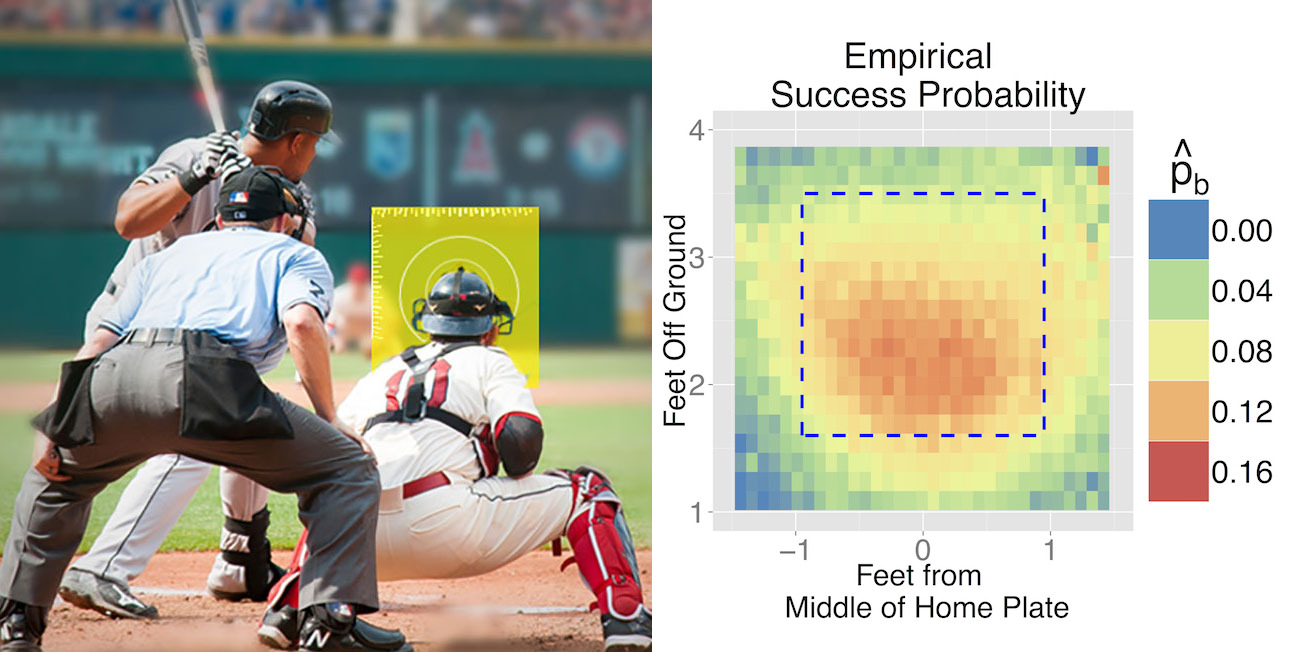
\includegraphics[scale=.35]{Images/SZandMothership.jpg} 
  \caption{The yellow square in the image on the left coincides with the dashed blue line in the heat map on the right. The heat map grids the vertical face of the hitting zone with approximately 3/4 inch by 3/4 inch boxes. Each grid box color maps $\hat{p}_{b}$---the empirical success probability of hitters swinging at pitches passing through that box---to a color.  The data consists of 1,932 right handed hitters, swinging at 1,582,581 pitches between 2008 and 2015.}
  \label{fig:ms}
	\end{figure} 
The graphic efficiently conveys spatial empirical success probabilities by mapping $\hat{p}_{b}$ to colors. However, note that the statistician determines the map's resolution.

\section{Traditional Heat Maps}

\subsection{Resolution} % ============== =============

By the time a viewer sees an empirical heat map, the analyst behind the graphic already chose a resolution. This important choice determines a uniform grid box size for the entire heat map, which influences its quality and appearance considerably. To understand this influence, consider histograms, where bin width selection similarly affects histogram appearance and function considerably. Small boxes may yield unreliable estimates at some locations, while larger boxes may fail to convey desired spatial specificity. 

Along these lines, note that heat maps conceal spatially varying data density. For example, the map in Figure \ref{fig:ms} gives no indication of the density of observations in different regions of the hitting zone. In this way, empirical heat maps also conceal sample sizes and estimate variances.  

With these points in mind, consider again the heat map in Figure \ref{fig:ms}. That heat map divides the hitting zone into relatively small boxes, because the data supports it; approximately 1.5 million swings by almost 2000 hitters. By ``supports it'' we mean that the small, spatially specific boxes at this resolution retain sample sizes large enough to supply reasonable estimates of $p_{b}$. ``Reasonable,'' of course, depends on context and objectives. For example, a pitching coach might request estimates within 0.005 points of the true batting average with probability 0.95. This requires a sample size of at least 36 when $p_{b} = 0.10$.\footnote{$\text{Var}(\hat{p}_{b})$ depends on $p_{b}$ This creates counterintuitive behavior around the margins of the hitting zone, where $\text{Var}(\hat{p}_{b})$ remains very small despite very small box sample sizes. See \cite{Dixon2005} for a discussion of this curious phenomenon.}

On the other hand, data for individual hitters varies dramatically in size. In our database, individual hitters range from a single swing to over 10,000 swings. At such varying scales, resolution selection becomes more complicated because non-uniform data density implies different regions may support very different resolutions. This is important because, as stated before, the choice of resolution sometimes dramatically affects heat map appearance, but also usefulness. For example, coarse resolution in regions of interest means the parameter estimates lose value. 

This important resolution decision usually depends on the size and nature of the data set, and its spatial dispersion through the domain. In the next section we explore resolution selection in detail, along with its inherent compromises.

\subsection{Resolution Selection}

In this section we use batter 425509, a veteran player named Jhonny Peralta, to explore resolution selection and its implications. The data includes 9,177 Peralta swings, which yields the heat map in Figure \ref{fig:4x4}. This map resolution divides the hitting zone into 16 equally sized boxes. Each box maps $\hat{p}_{b}$ to a color, with box sample sizes, $n_{b}$, printed on box centers. We will use box sample sizes to reference boxes. For example, we will call the box in the lower-left ``box 22.'' 
        \begin{figure}[H]
      	\centering
      	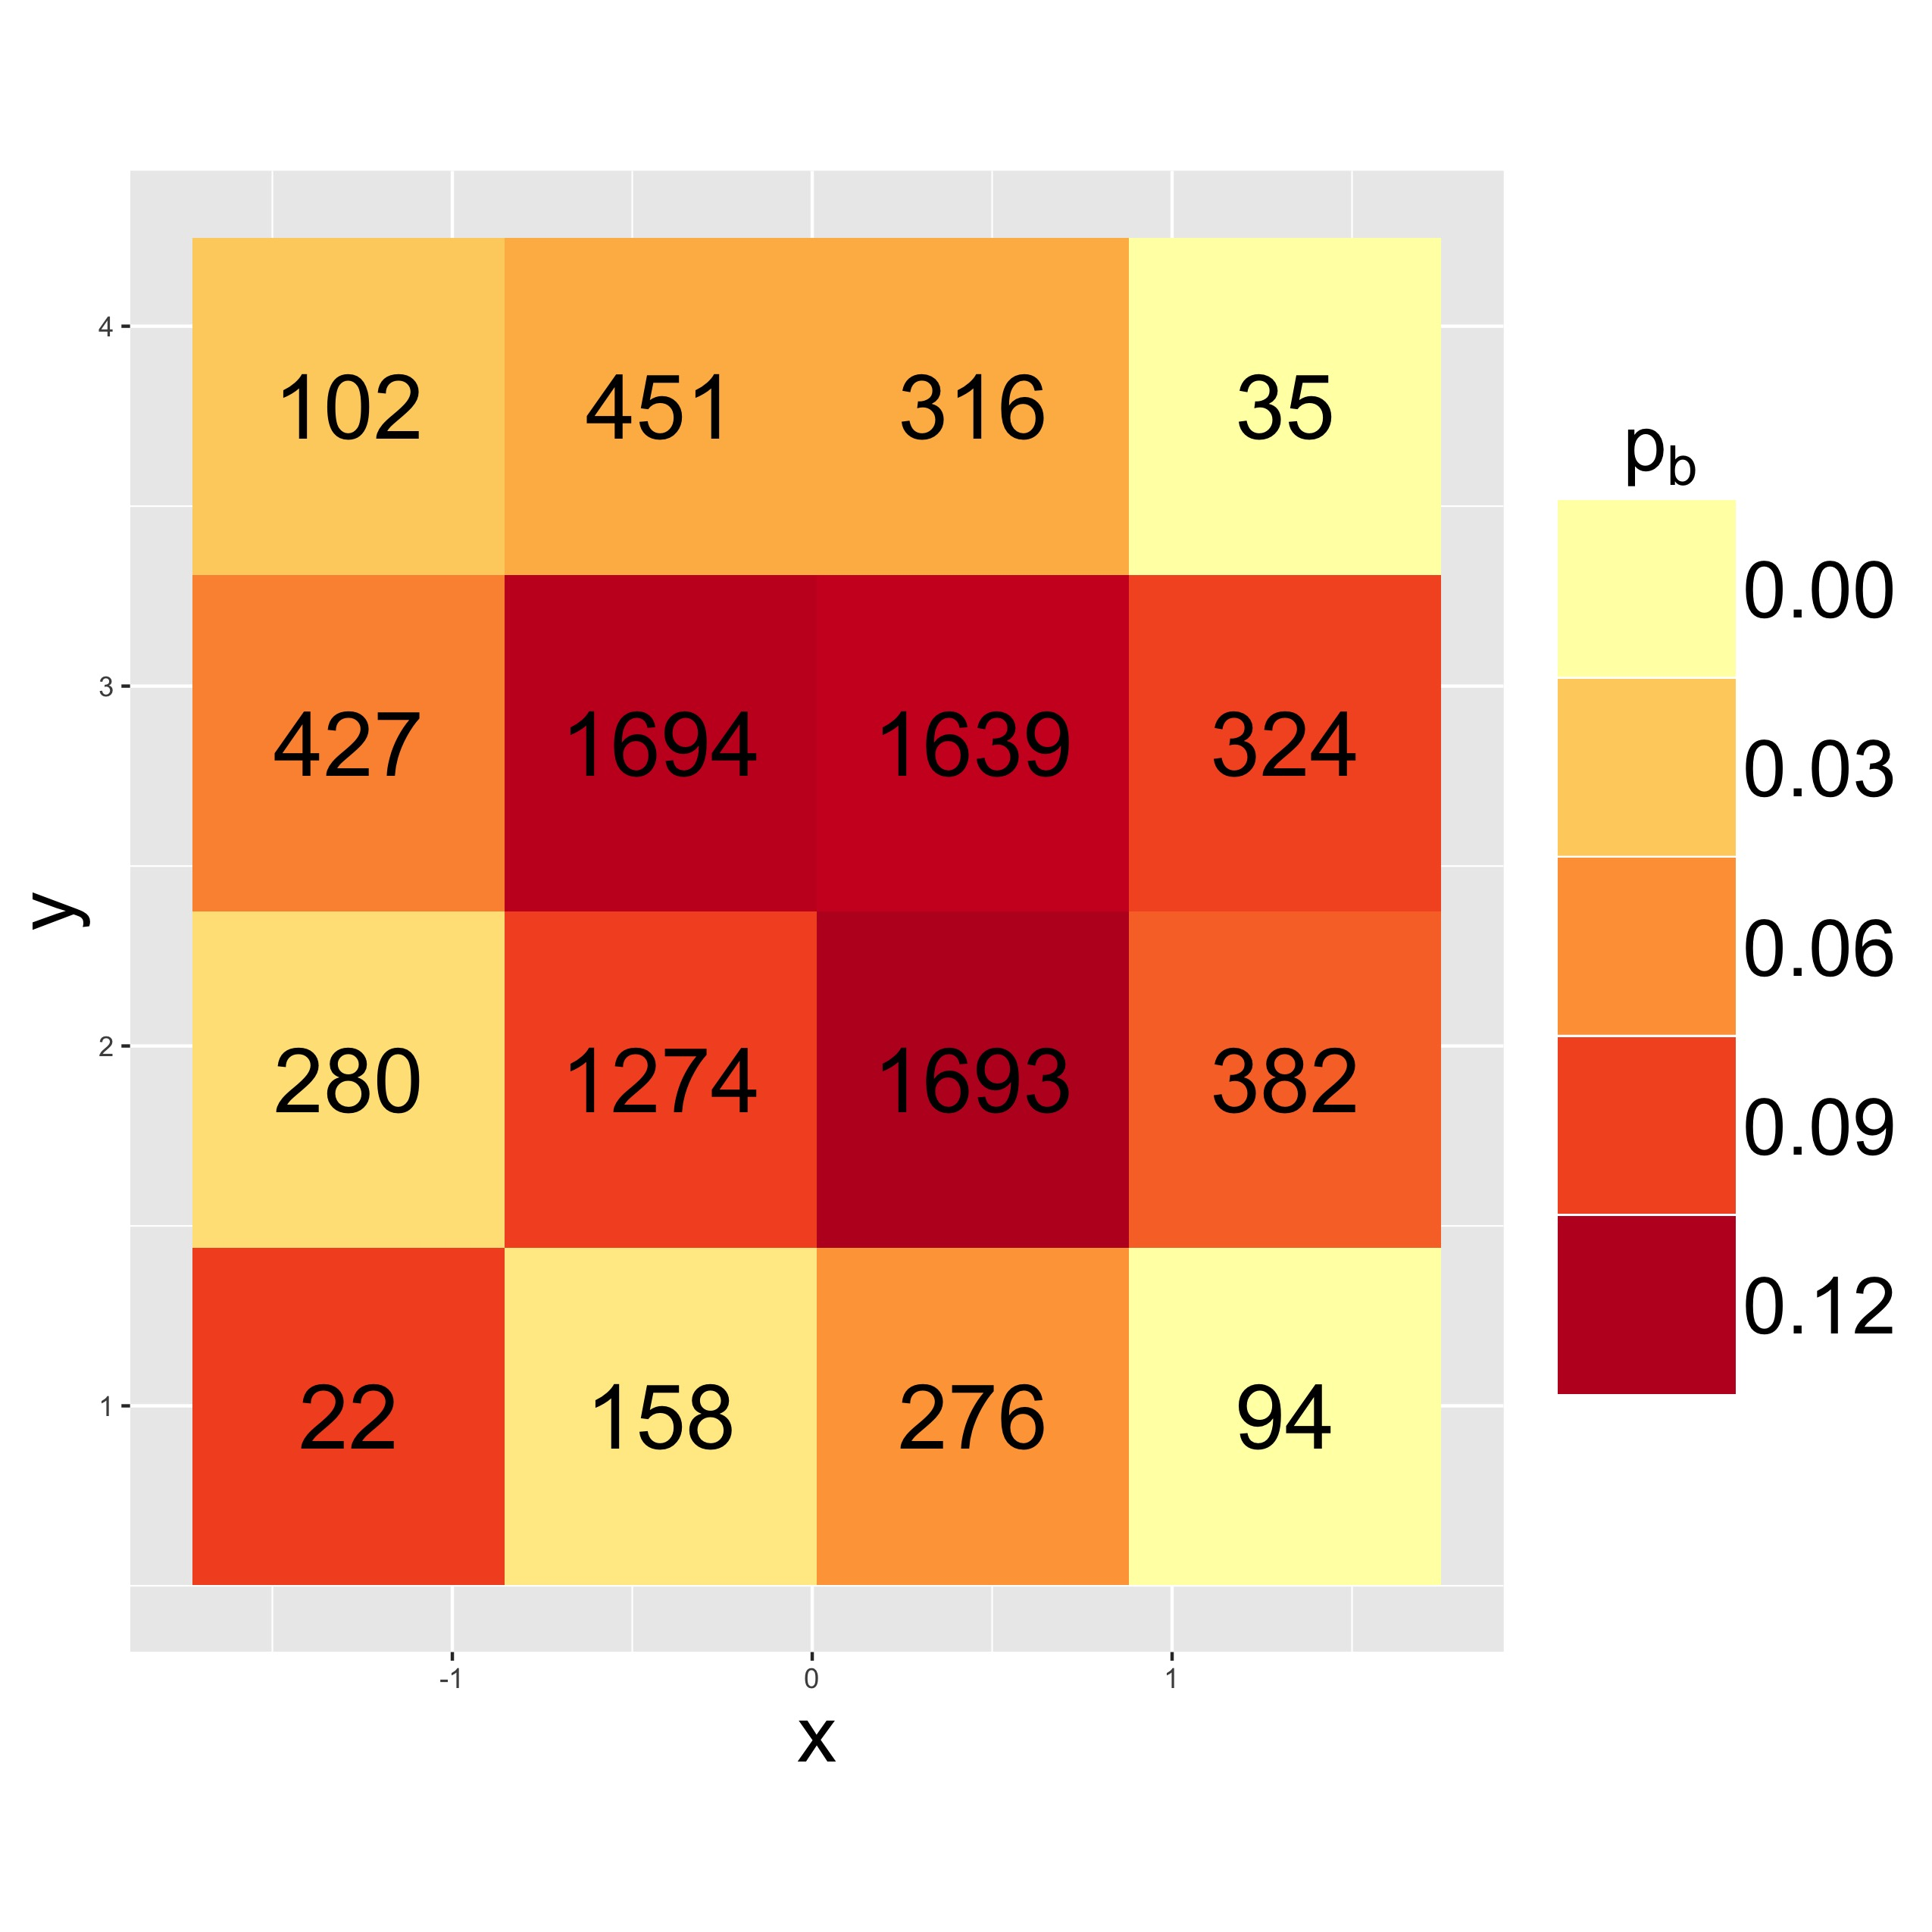
\includegraphics[scale=.1]{Images/Chapter4x4.jpg} 
      	\caption{This four by four heat map shows the empirical batting average of Jhonny Peralta, for pitches passing through the space represented by each of 16 square regions of the hitting zone. Each box maps $\hat{p}_{b}$ to a color, with box sample sizes, $n_{b}$, printed on box centers.}
      	\label{fig:4x4}
      	\end{figure} 

Notice that while the four by four resolution suffices for box 22, further subdivision might yield trivially small sample sizes. On the other hand, the four central boxes, all with sample sizes above 1200, can and should contribute more location-specific estimates. Therefore, the central boxes motivate finer resolution, even though box 22 does not support it. Keeping this trade-off in mind, we increase resolution by dividing each box into four equally sized sub-boxes. Figure \ref{fig:8x8} shows the $8 \times 8$ resolution result.
        \begin{figure}[H]
      	\centering
      	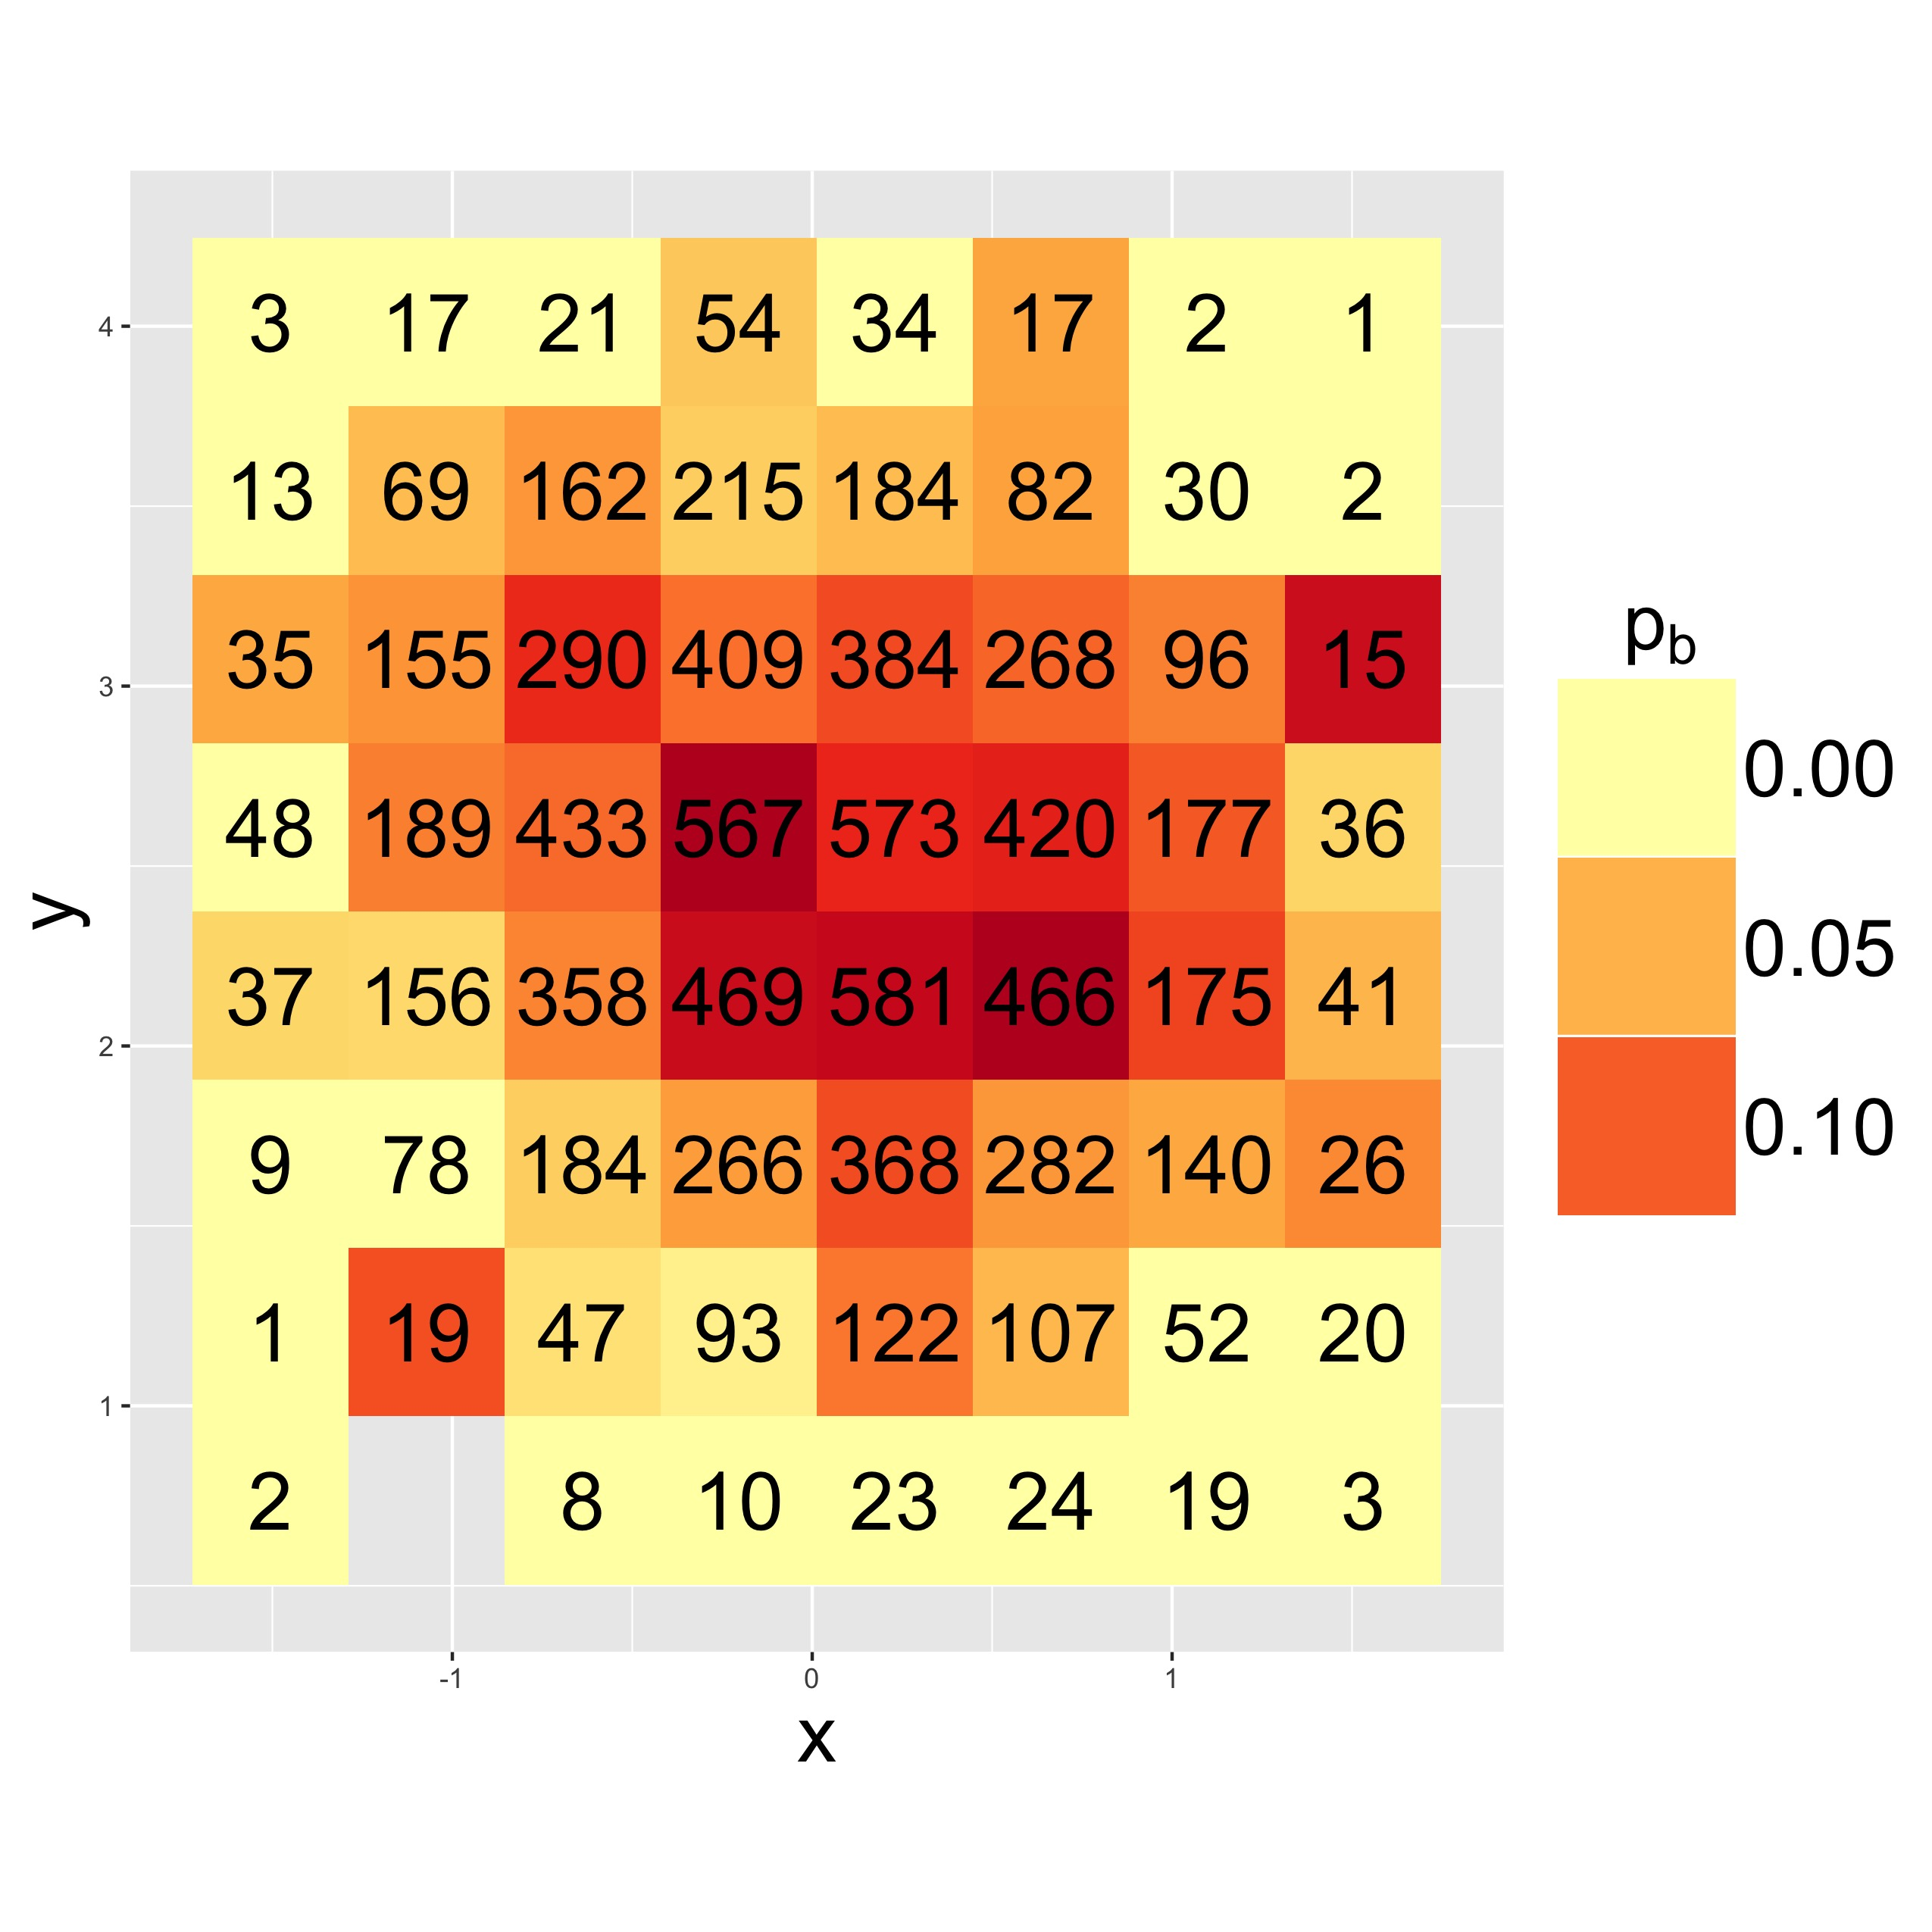
\includegraphics[scale=.1]{Images/Chapter8x8.jpg} 
      	\caption{This eight by eight heat map shows the empirical hitting success probability of Jhonny Peralta, for pitches passing through the space represented by each of 64 square regions of the hitting zone. Each box maps $\hat{p}_{b}$ to a color, with box sample sizes, $n_{b}$, printed on box centers. A grey box indicates no pitches passed through that box. Notice that this resolution imparts additional information in the center of the hitting zone, but some box sample sizes near the margins have dropped uninformatively low.}
      	\label{fig:8x8}
      	\end{figure} 
The centermost 16 boxes still support low variance $p$ estimates; the minimum of these boxes contains 184 swings. Globally, 24 boxes consist of over 150 swings; and 15 boxes still include more than than 250 swings. These boxes could support higher resolution. On the other hand, many boxes, especially edge boxes, now contain sample sizes generally insufficient to support low variance estimates of $p_{b}$. Twenty-nine boxes contain fewer than 50 swings, and 17 boxes contain fewer than 20 swings. One box recorded zero swings.

With this range of box sample sizes, the non-extreme resolution choices contain both boxes with exceedingly small sample sizes {\it and} boxes with unnecessarily large sample sizes. Figure \ref{fig:6res} shows Peralta's data---the same data---at six resolutions. 
        \begin{figure}[H]
      	\centering
      	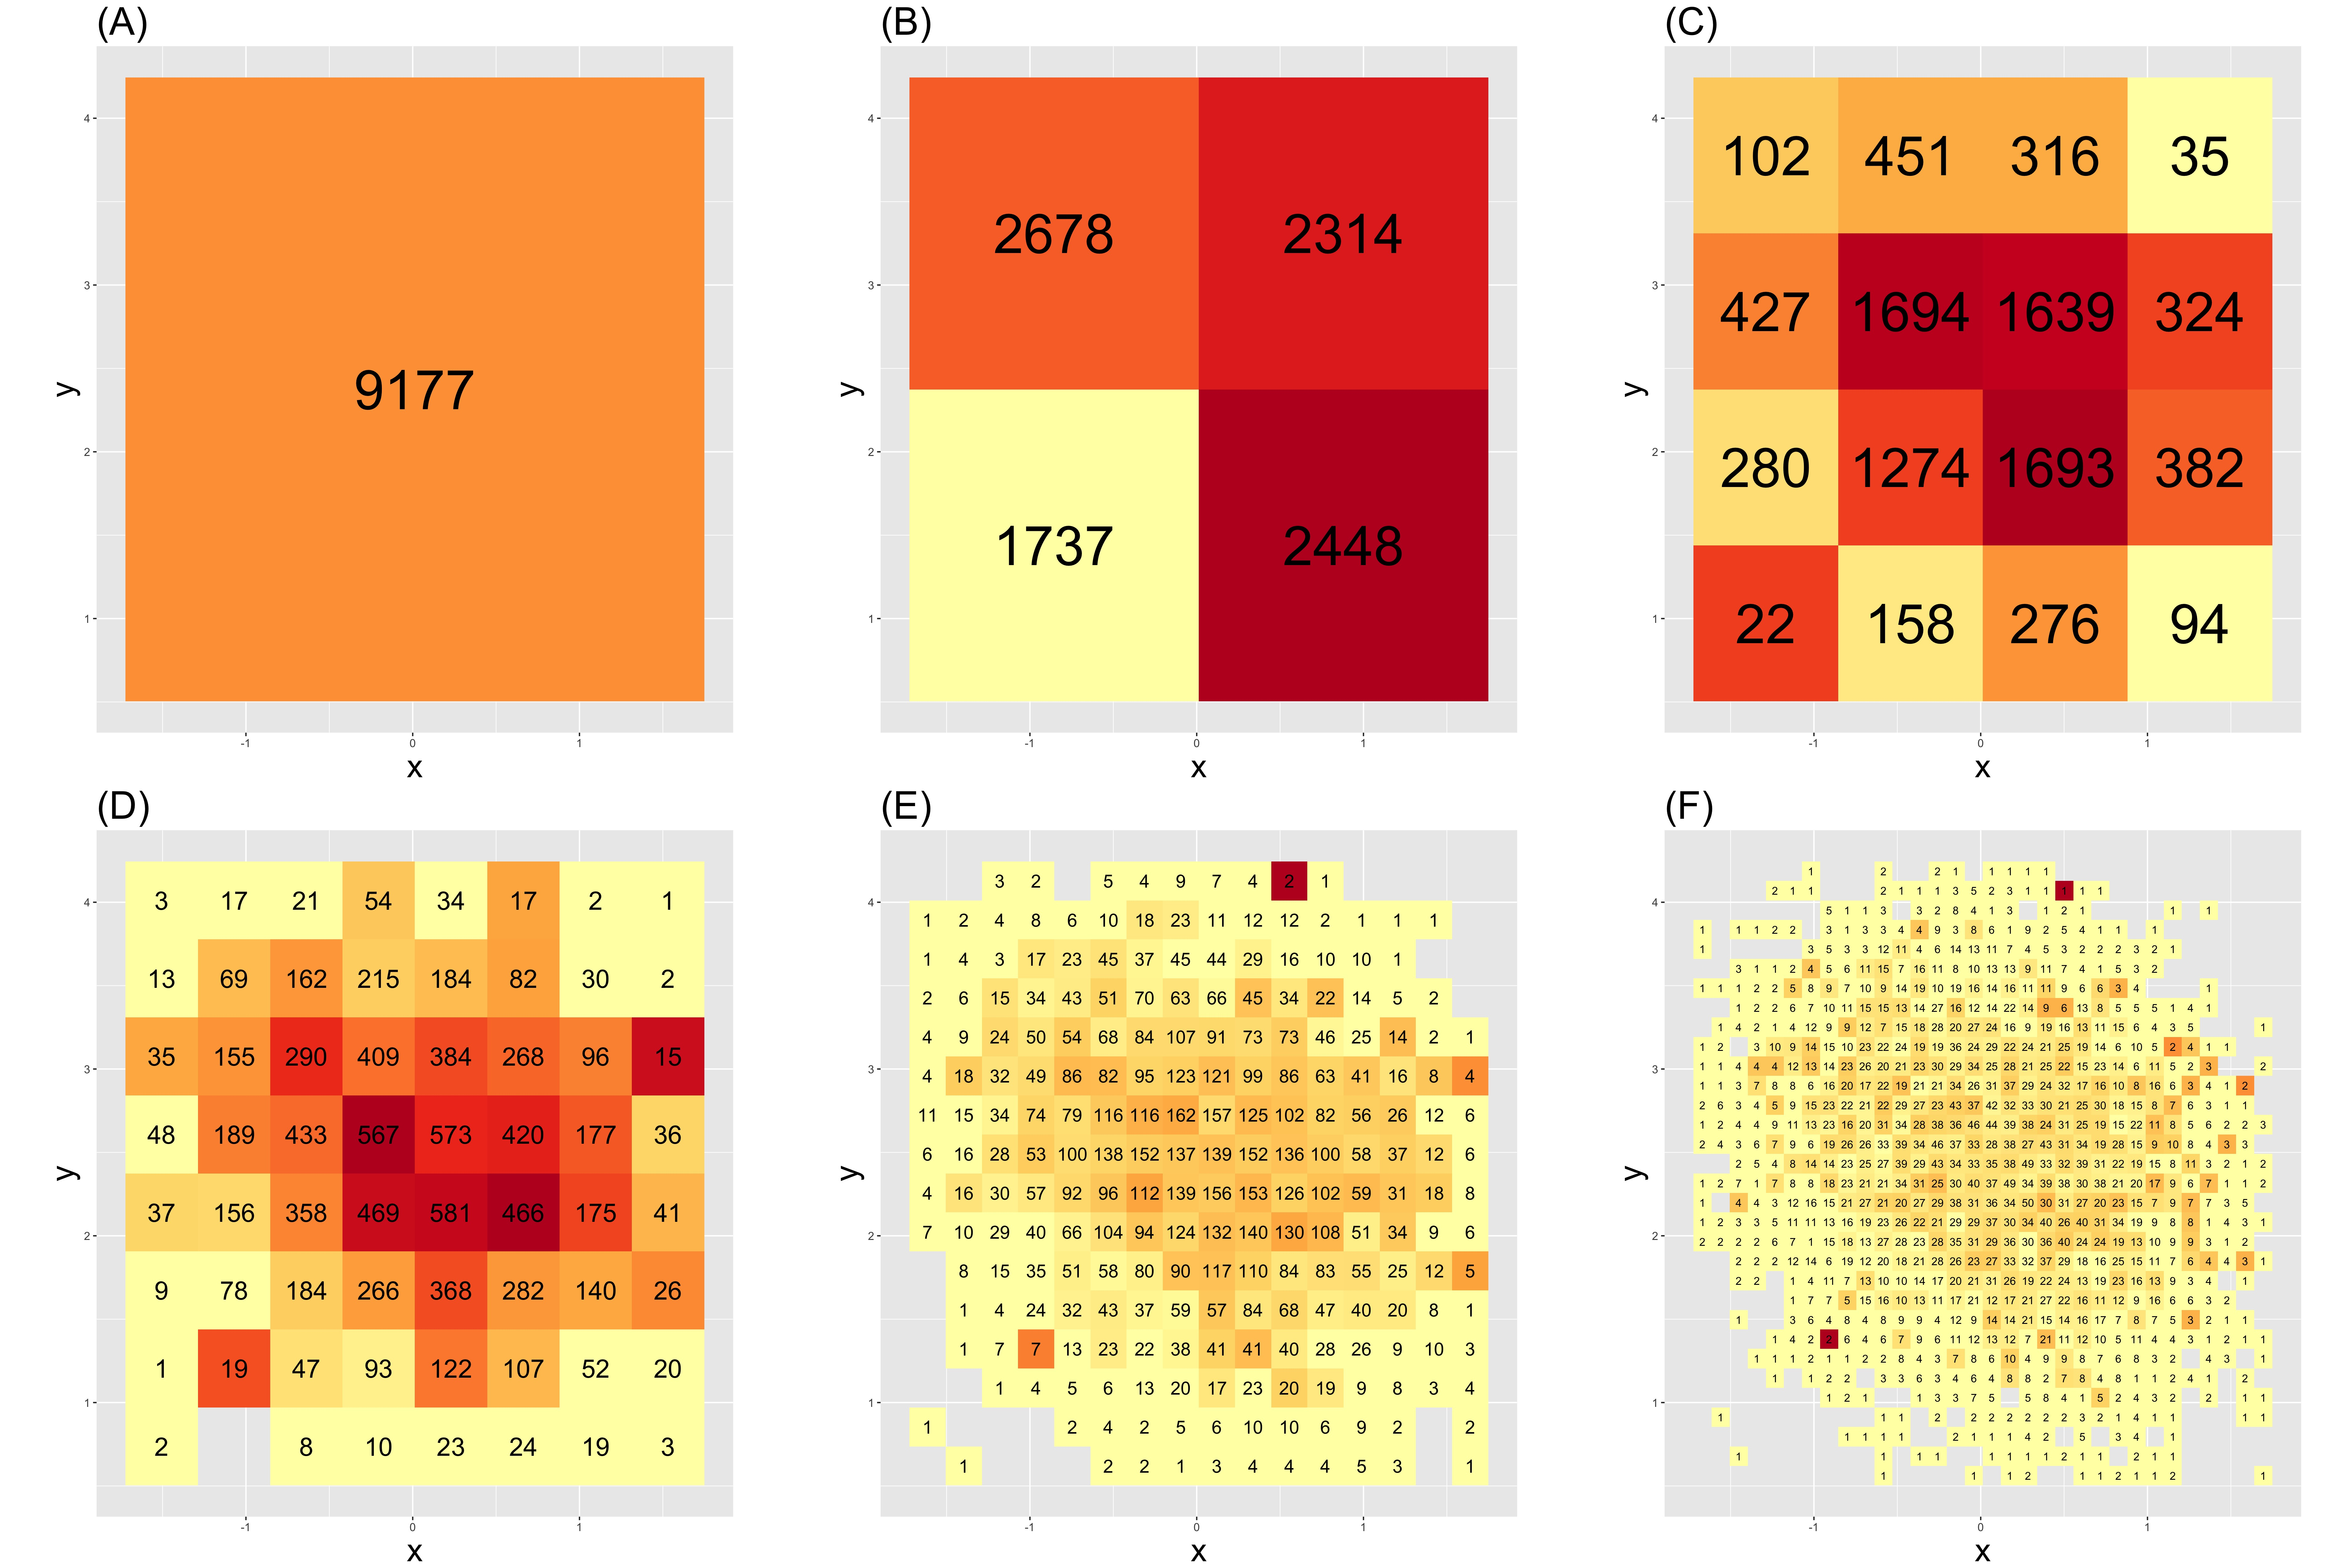
\includegraphics[scale=.055]{Images/Chapter_VarRes.jpg} 
      	\caption{These six heat maps show the same data for Jhonny Peralta, at increasing resolutions. The maps range from too coarse to too fine. Notice how dramatically the image changes as the resolution increases. Which resolution yields the highest quality heat map?}
      	\label{fig:6res}
      	\end{figure} 
We started with one box, and then subdivided each box into four equally-sized, smaller boxes at each iteration. Which of these six resolutions best balances spatially precise estimates of $p$ with acceptable box sample sizes? The user interested in the center of the strike zone might prefer the bottom-middle map, as the box sample sizes support such spatially specific estimates. However, the boxes closer to the edges of the strike zone then contain prohibitively small sample sizes, yielding higher variance estimates. 

The takeaway from Figure \ref{6res}: all six resolutions involve trade-offs. We propose a new heat map approach that eliminates trade-offs. The solution combines multiple resolutions into one map, according to the data's varying spatial density.

\section{Variable-Resolution Heat Maps} 

\subsection{The Varying Resolution Solution}

Consider again the Peralta $4 \times 4$ heat map in Figure \ref{fig:4x4}. Recall box 22 contains 22 swings, a sample size where subdividing further yields uninformatively small sample sizes. In contrast, box 1694 would support estimates that are more spatially accurate without $\text{Var}(\hat{p}_{b})$ increasing beyond acceptable levels. To resolve this problem, we propose deciding resolution increases algorithmically, box by box, with a stopping rule; we christen it the variable-resolution (VR) algorithm. The map's author chooses a stopping rule, giving him/her the flexibility to create the heat map that suits the data. 

To demonstrate one iteration in the VR algorithm, let the stopping rule be a maximum box sample size of 200, and recall the $4 \times 4$ map in Figure \ref{fig:4x4} (Figure \ref{fig:4x4and8x8}, left). On this map we divide all boxes where $n_{b} > 200$, into four smaller, equally sized boxes. Figure \ref{fig:4x4and8x8} shows the map before and after. Moving through all boxes of the map to the left, subdividing when $n_{b} > 200$, yields the heat map to the right.
        \begin{figure}[H]
      	\centering
      	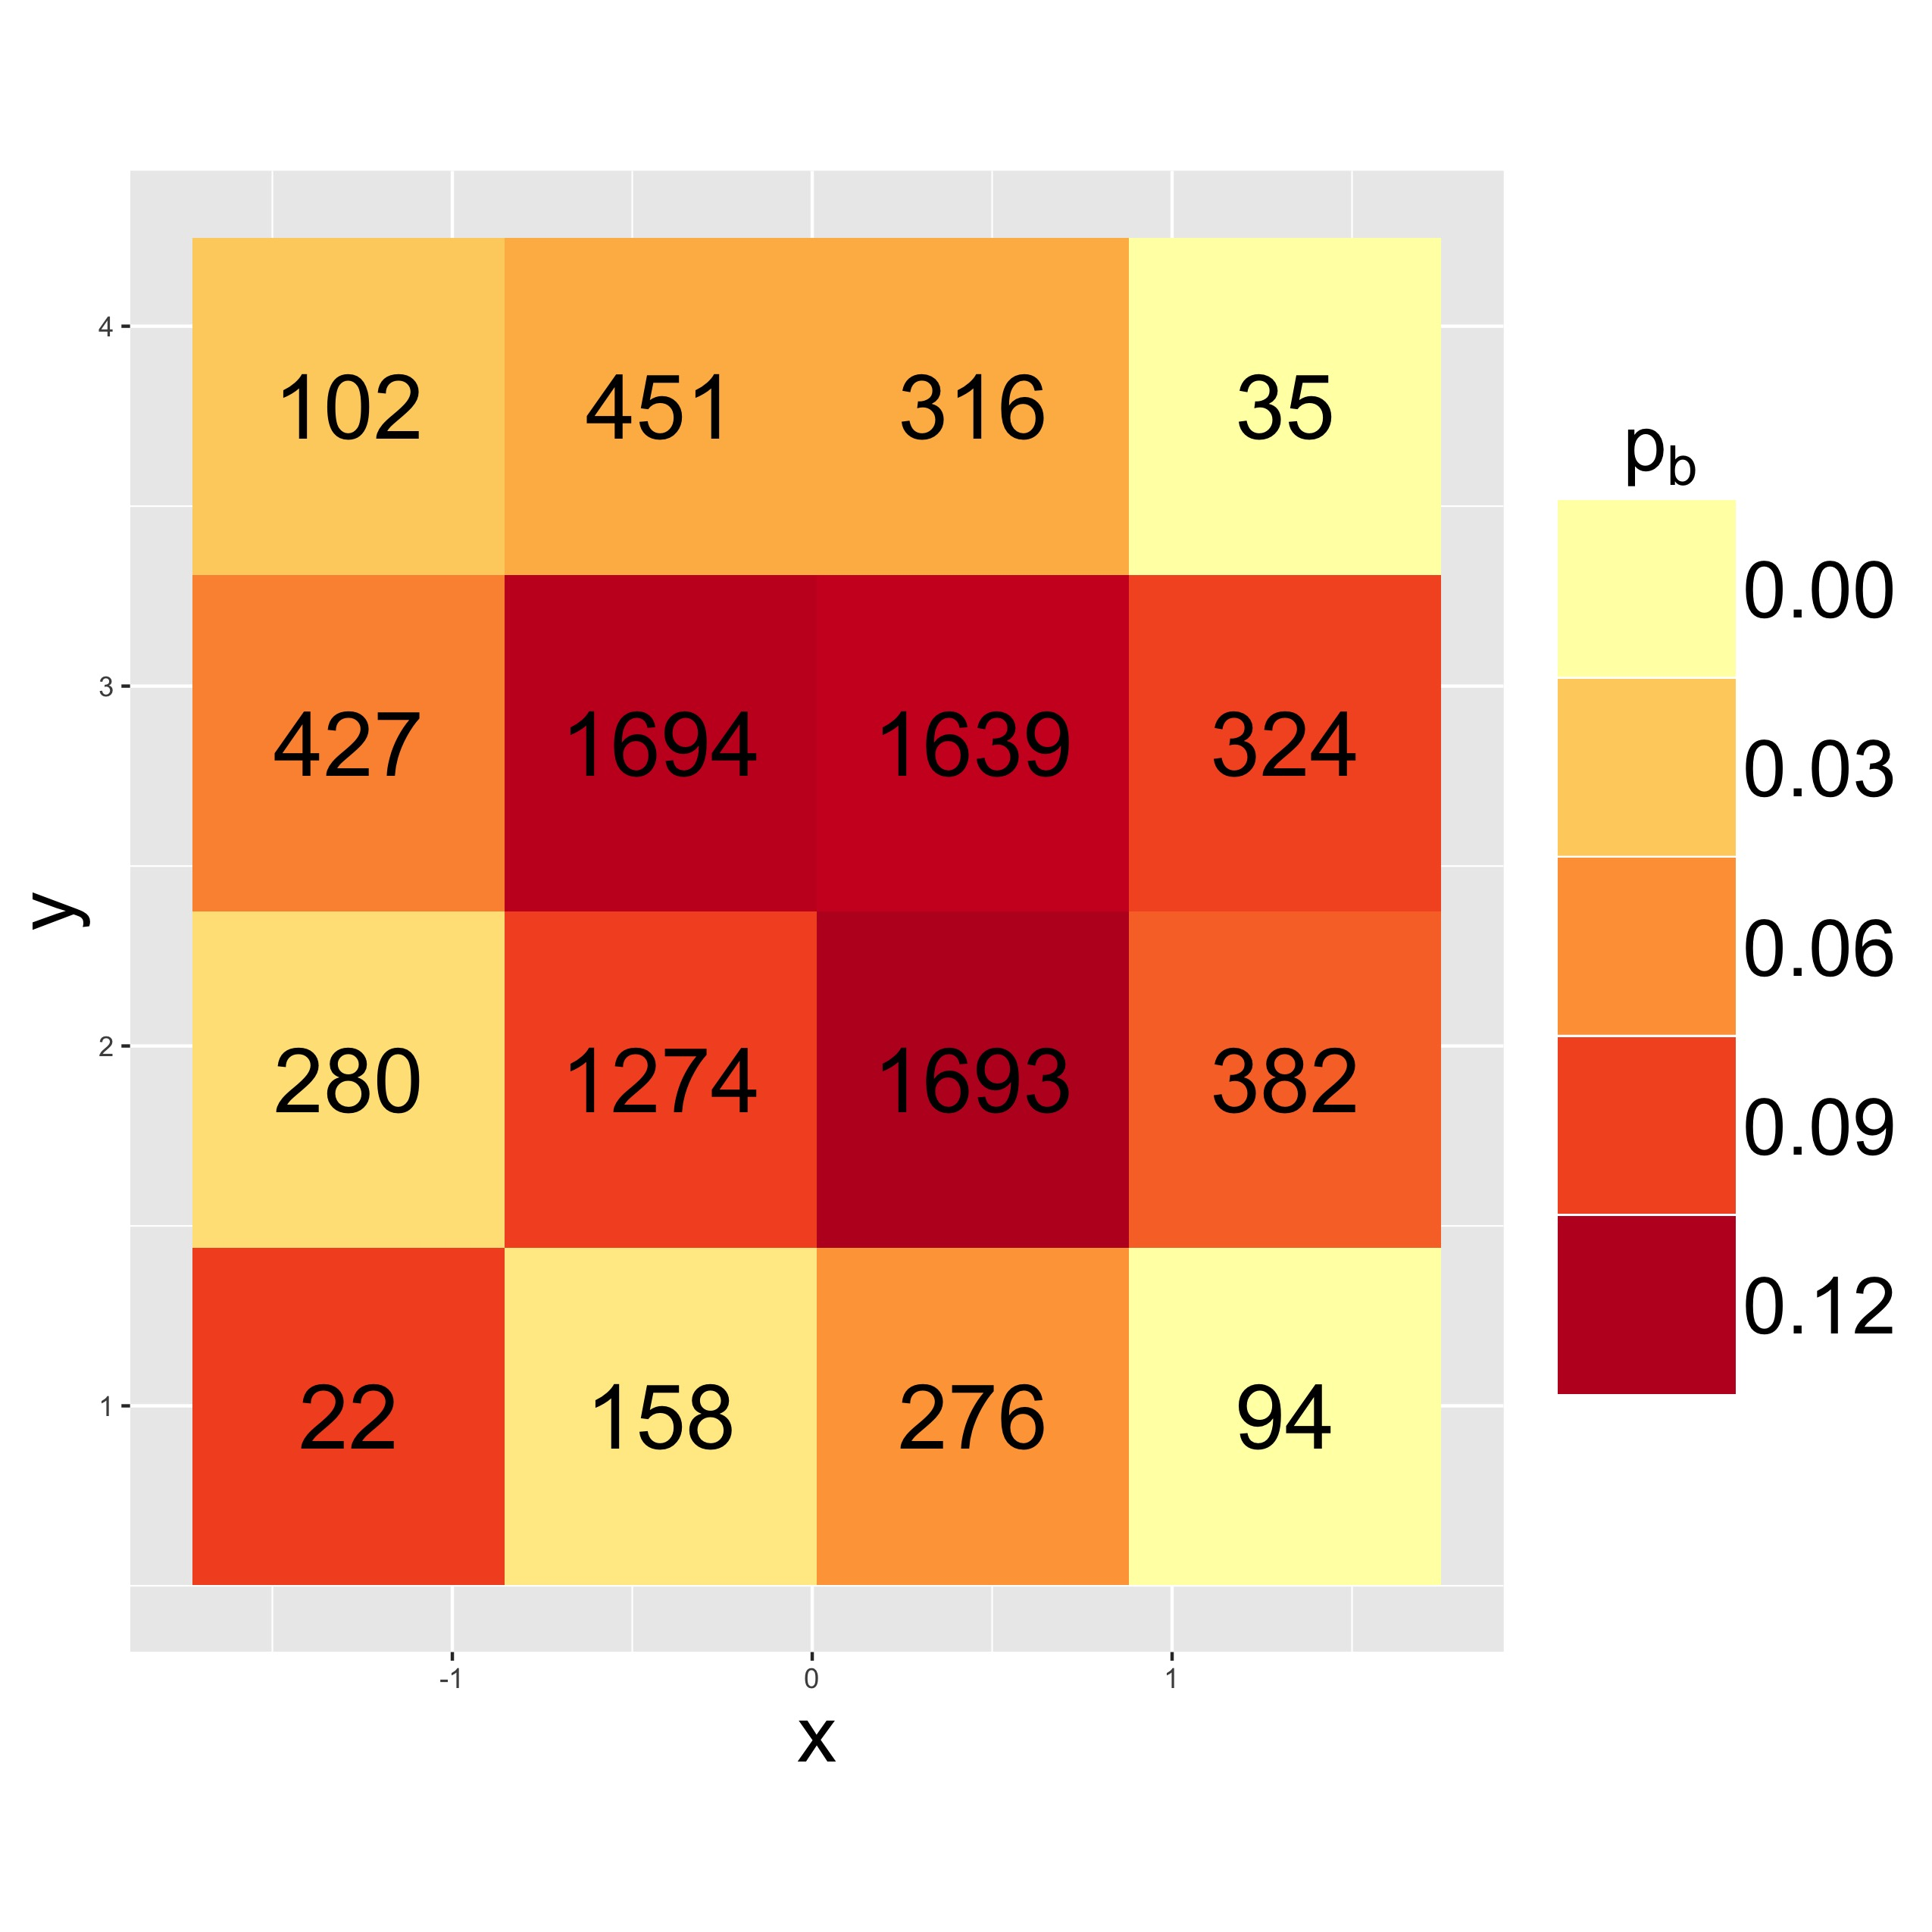
\includegraphics[scale=.08]{Images/Chapter4x4.jpg} 
      	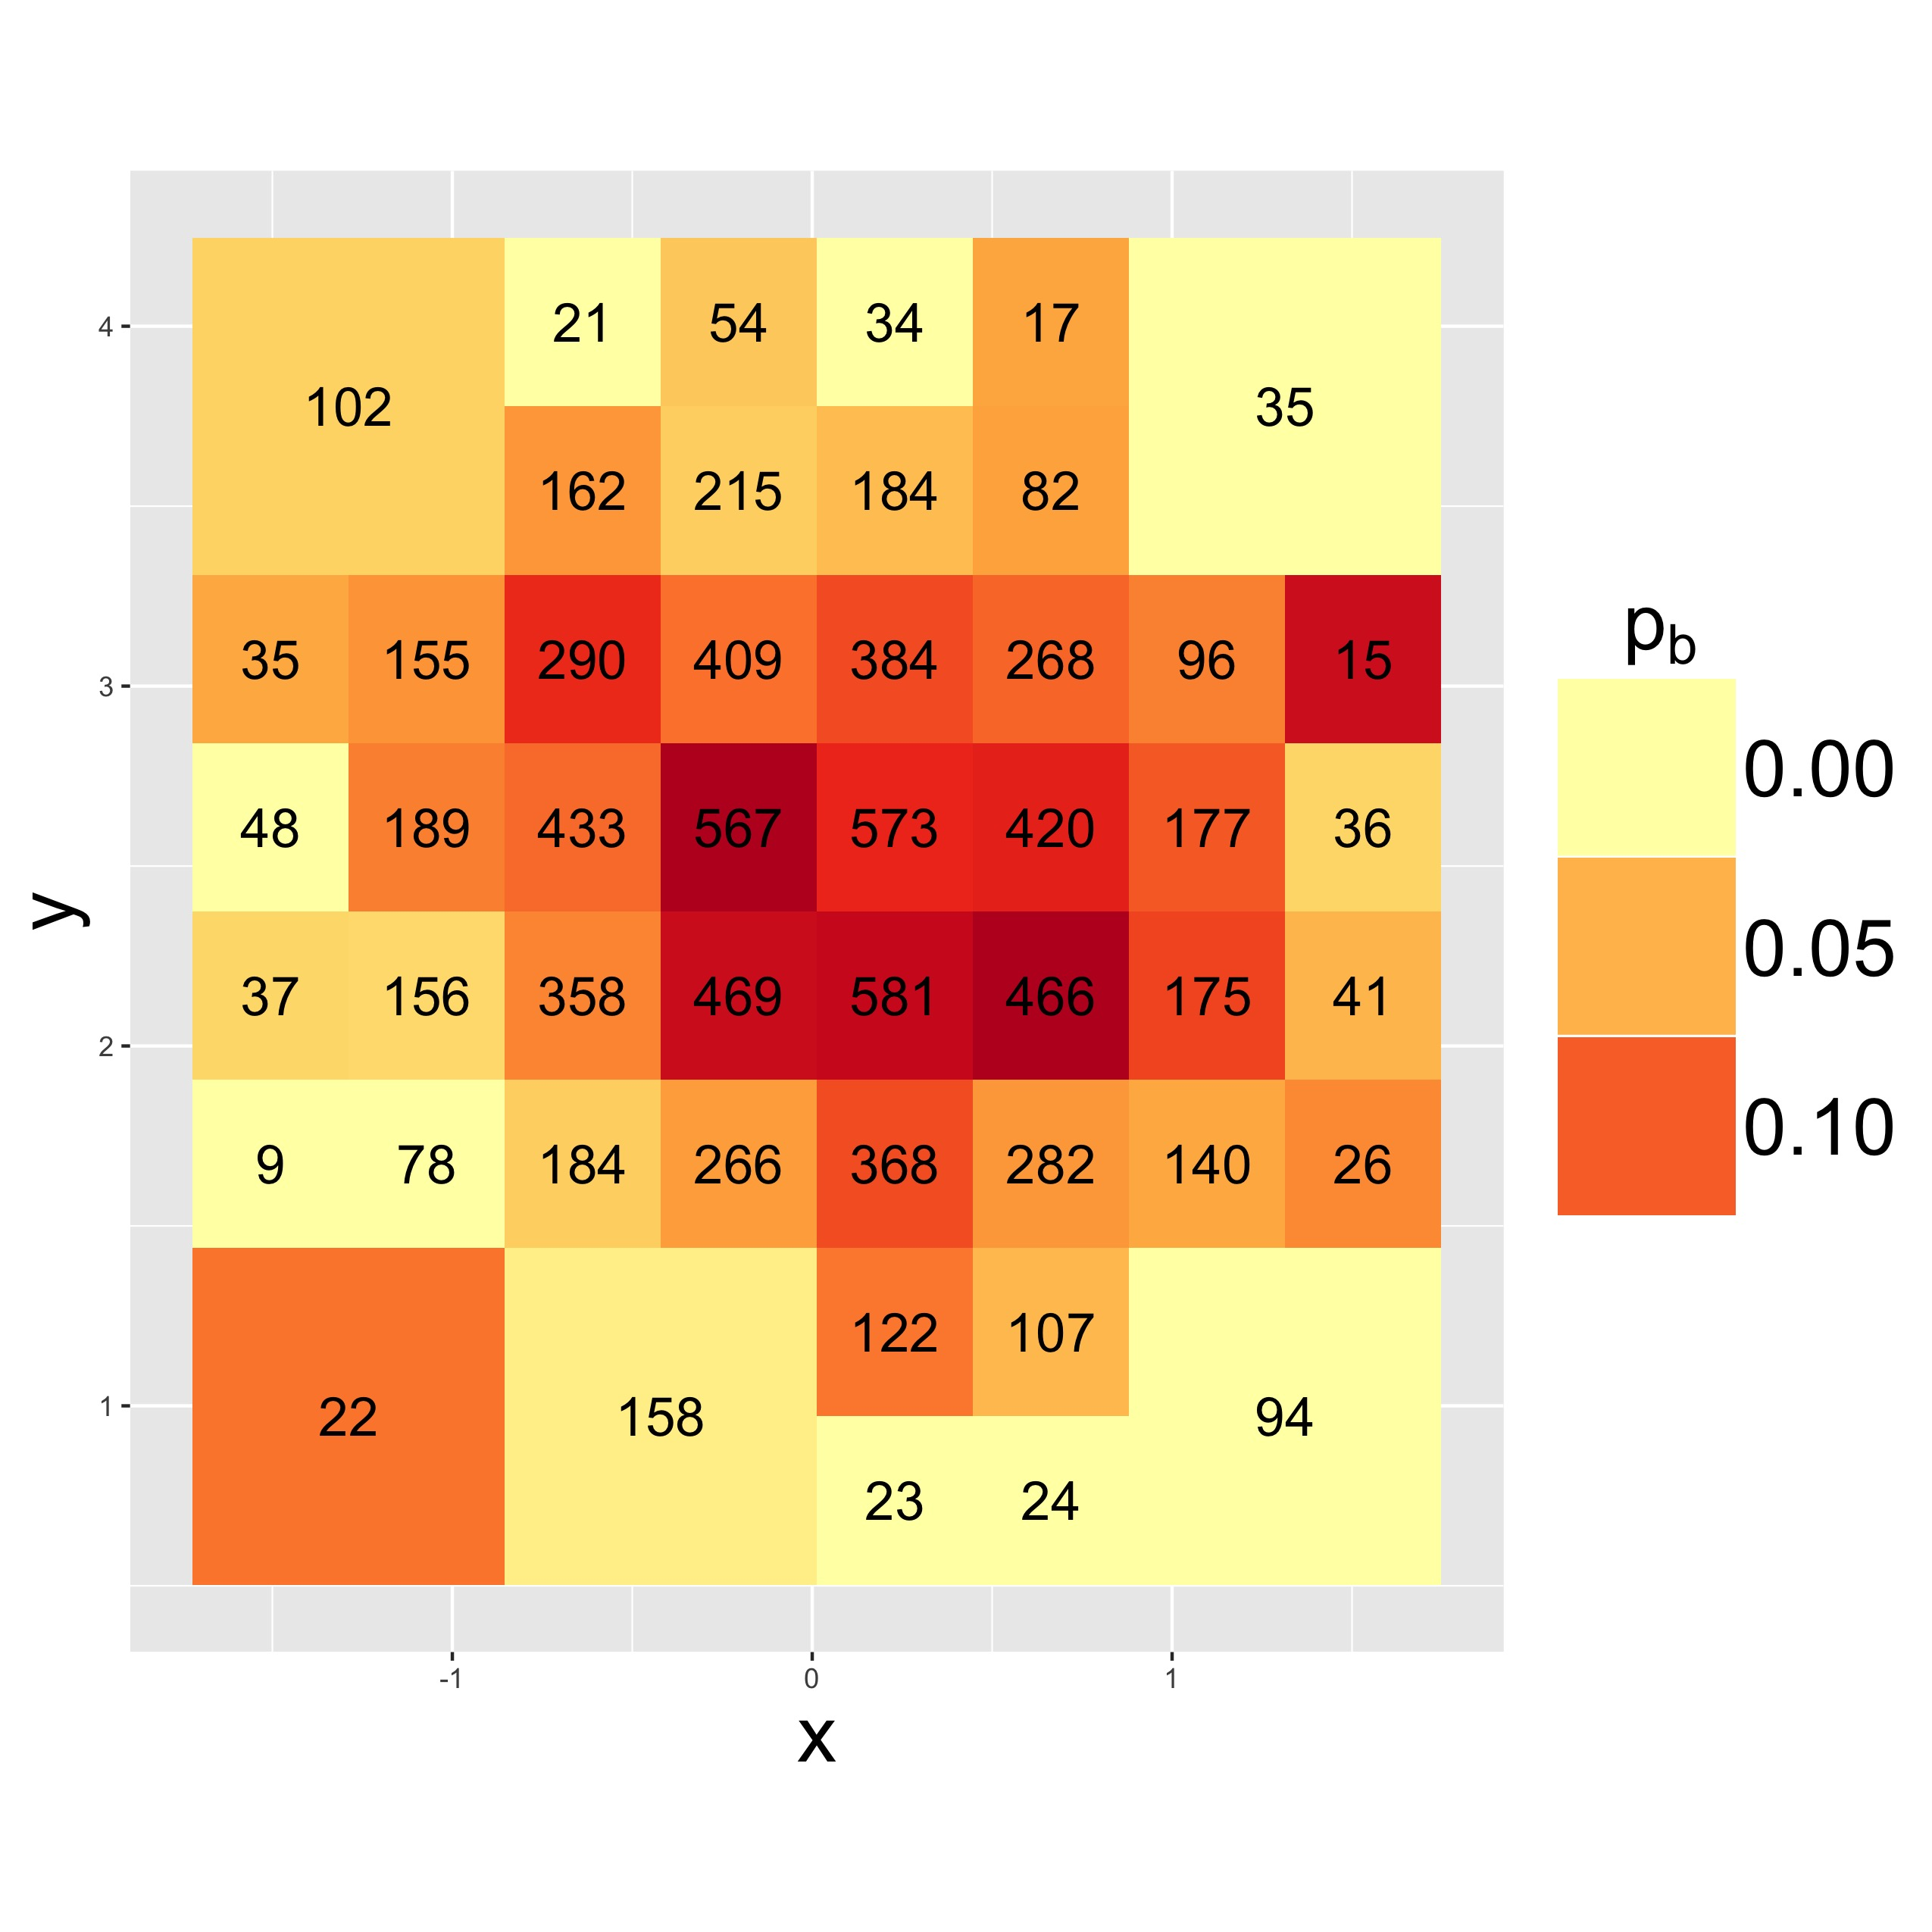
\includegraphics[scale=.08]{Images/Chapter8x8_200.jpg} 
      	\caption{One iteration in the variable-resolution algorithm. The algorithm subdivides all boxes with a sample size (printed on box) greater than 200. The iteration shown here yields the map on the right, from the map on the left. Box 22, and others like it, remain intact because further subdivision yields uninformatively low sample sizes.}
      	\label{fig:4x4and8x8}
      	\end{figure} 
The algorithm subdivides all boxes that have more than 200 observations, yielding the heat map on the right. Boxes with less than 200 observations, such as box 22, remain intact because further subdivision yields sample sizes the hypothetical author deems uninformative. Sixteen boxes still contain a sample size greater than 200, and 11 still have a sample size greater than 300. The next algorithmic iteration subdivides all 16 boxes that still contain more than 200 observations. 
        \begin{figure}[H]
      	\centering
      	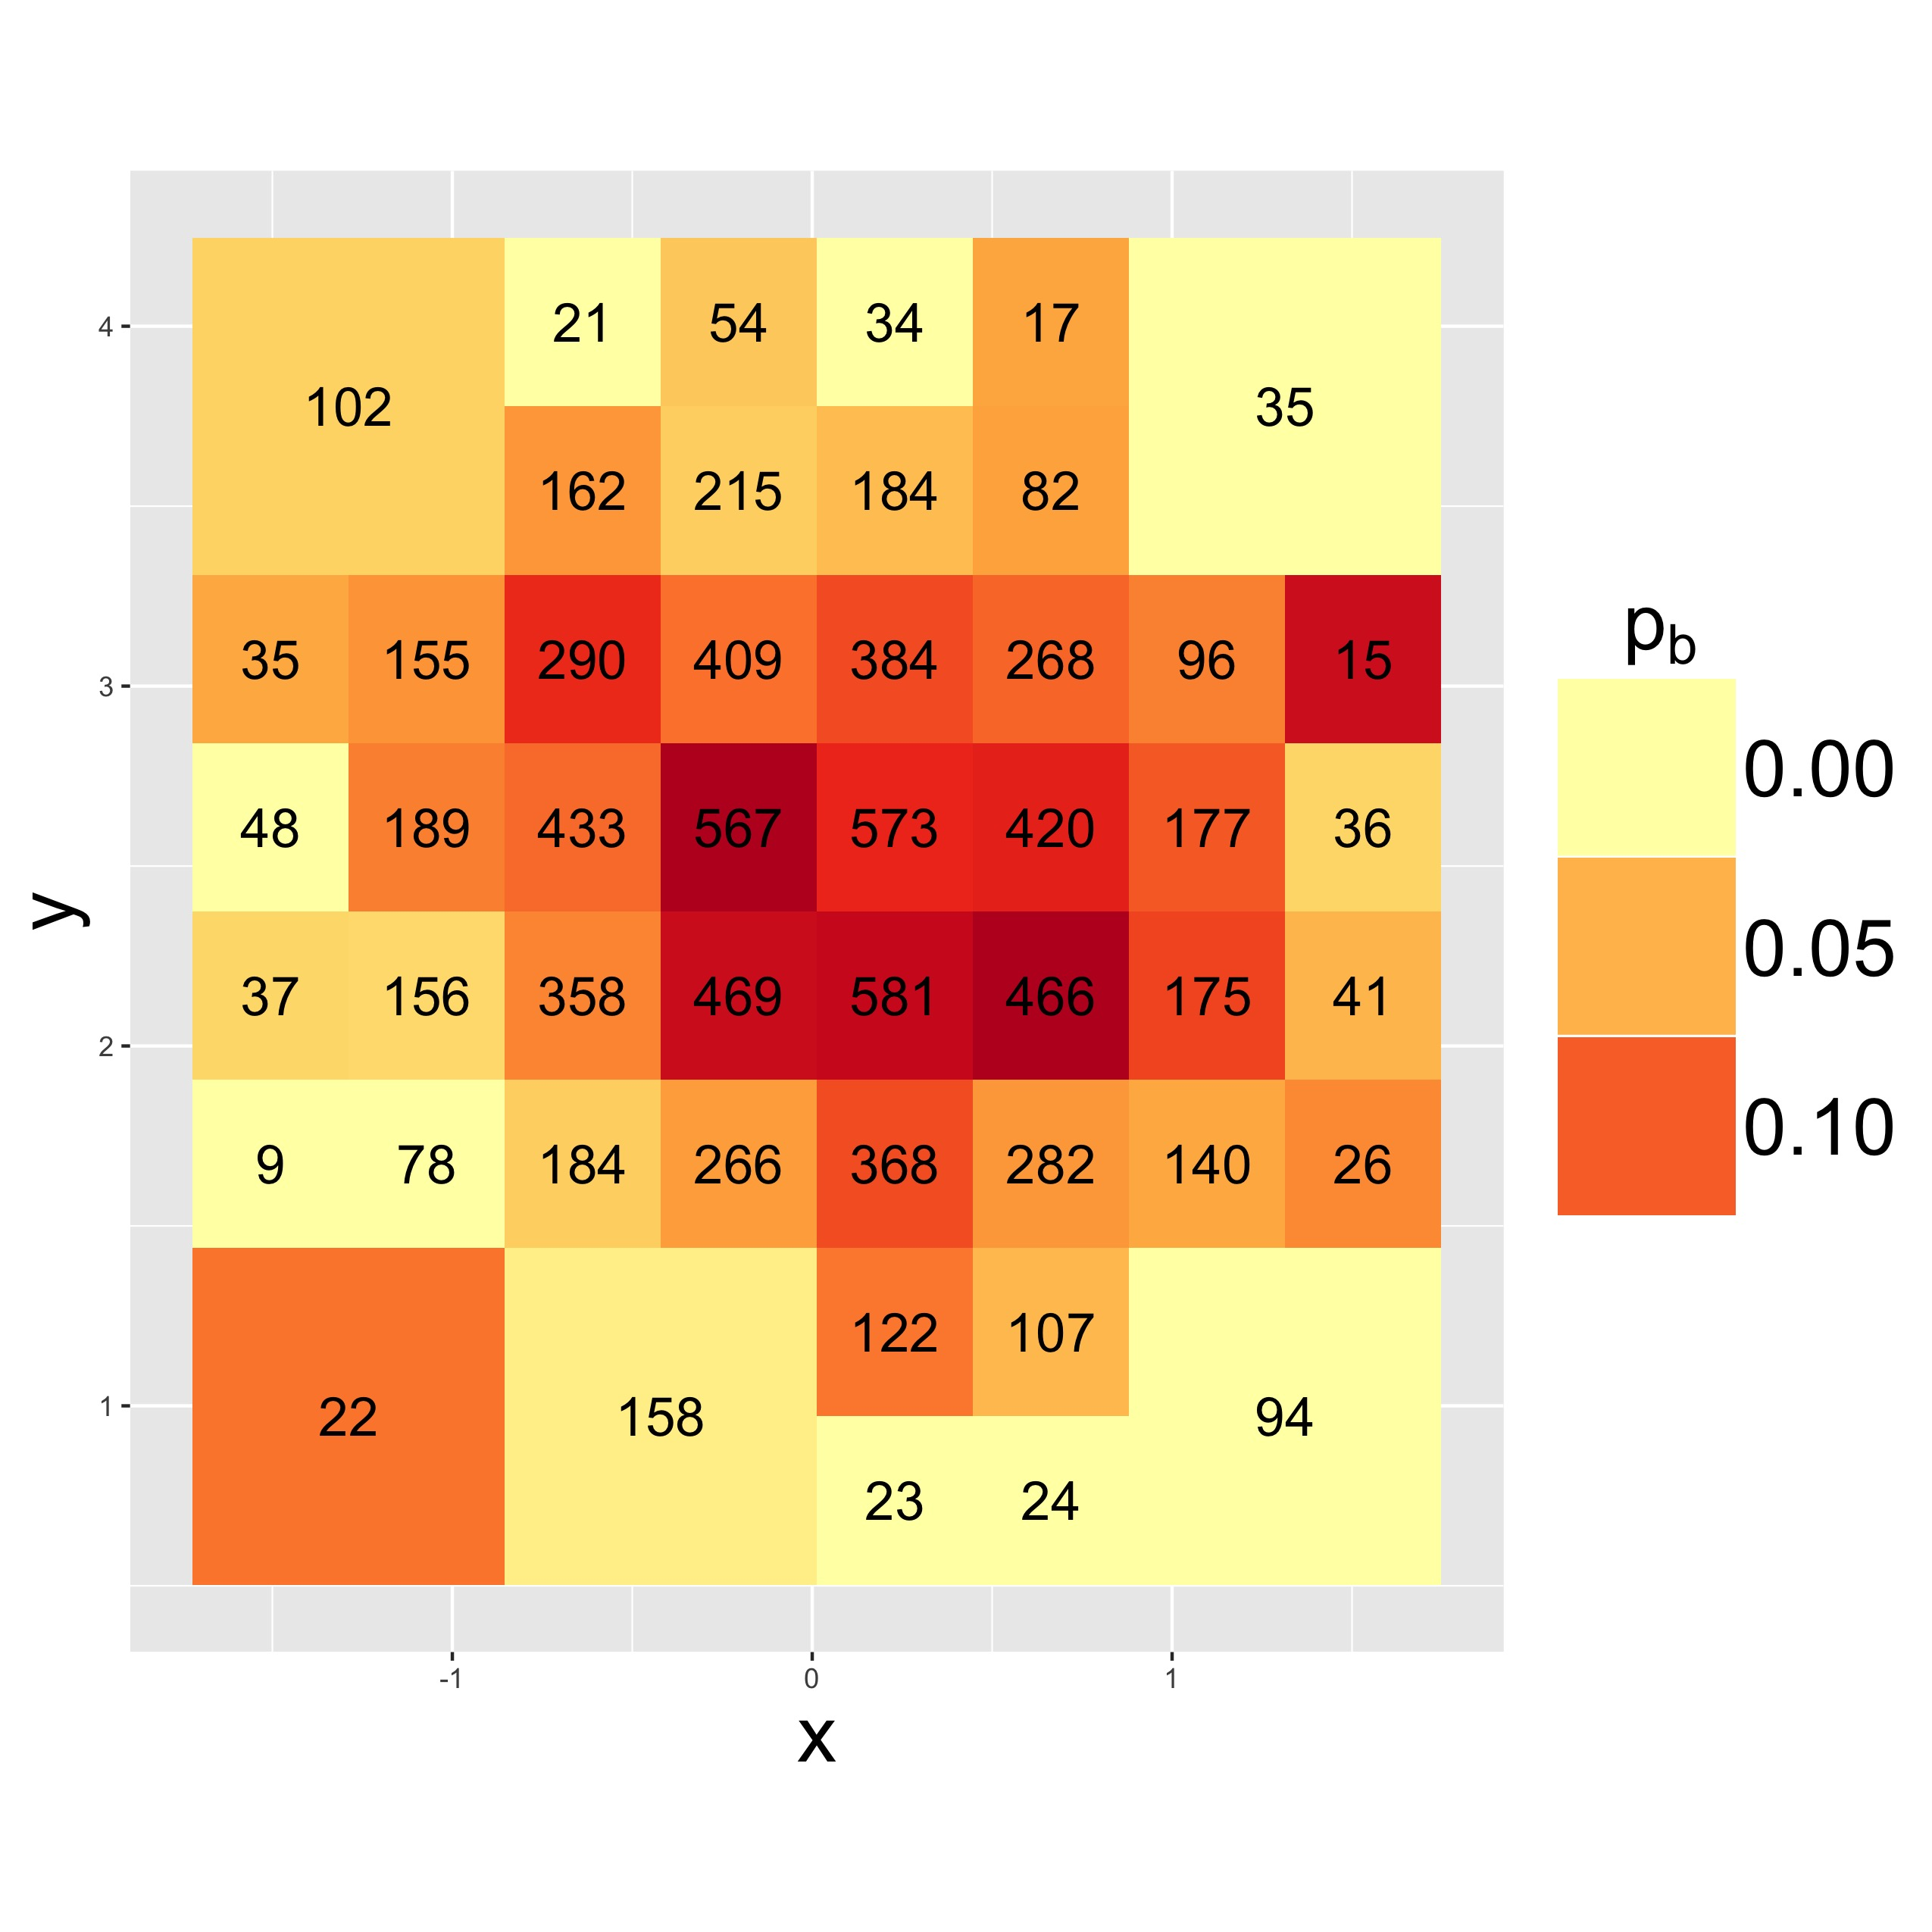
\includegraphics[scale=.08]{Images/Chapter8x8_200.jpg} 
      	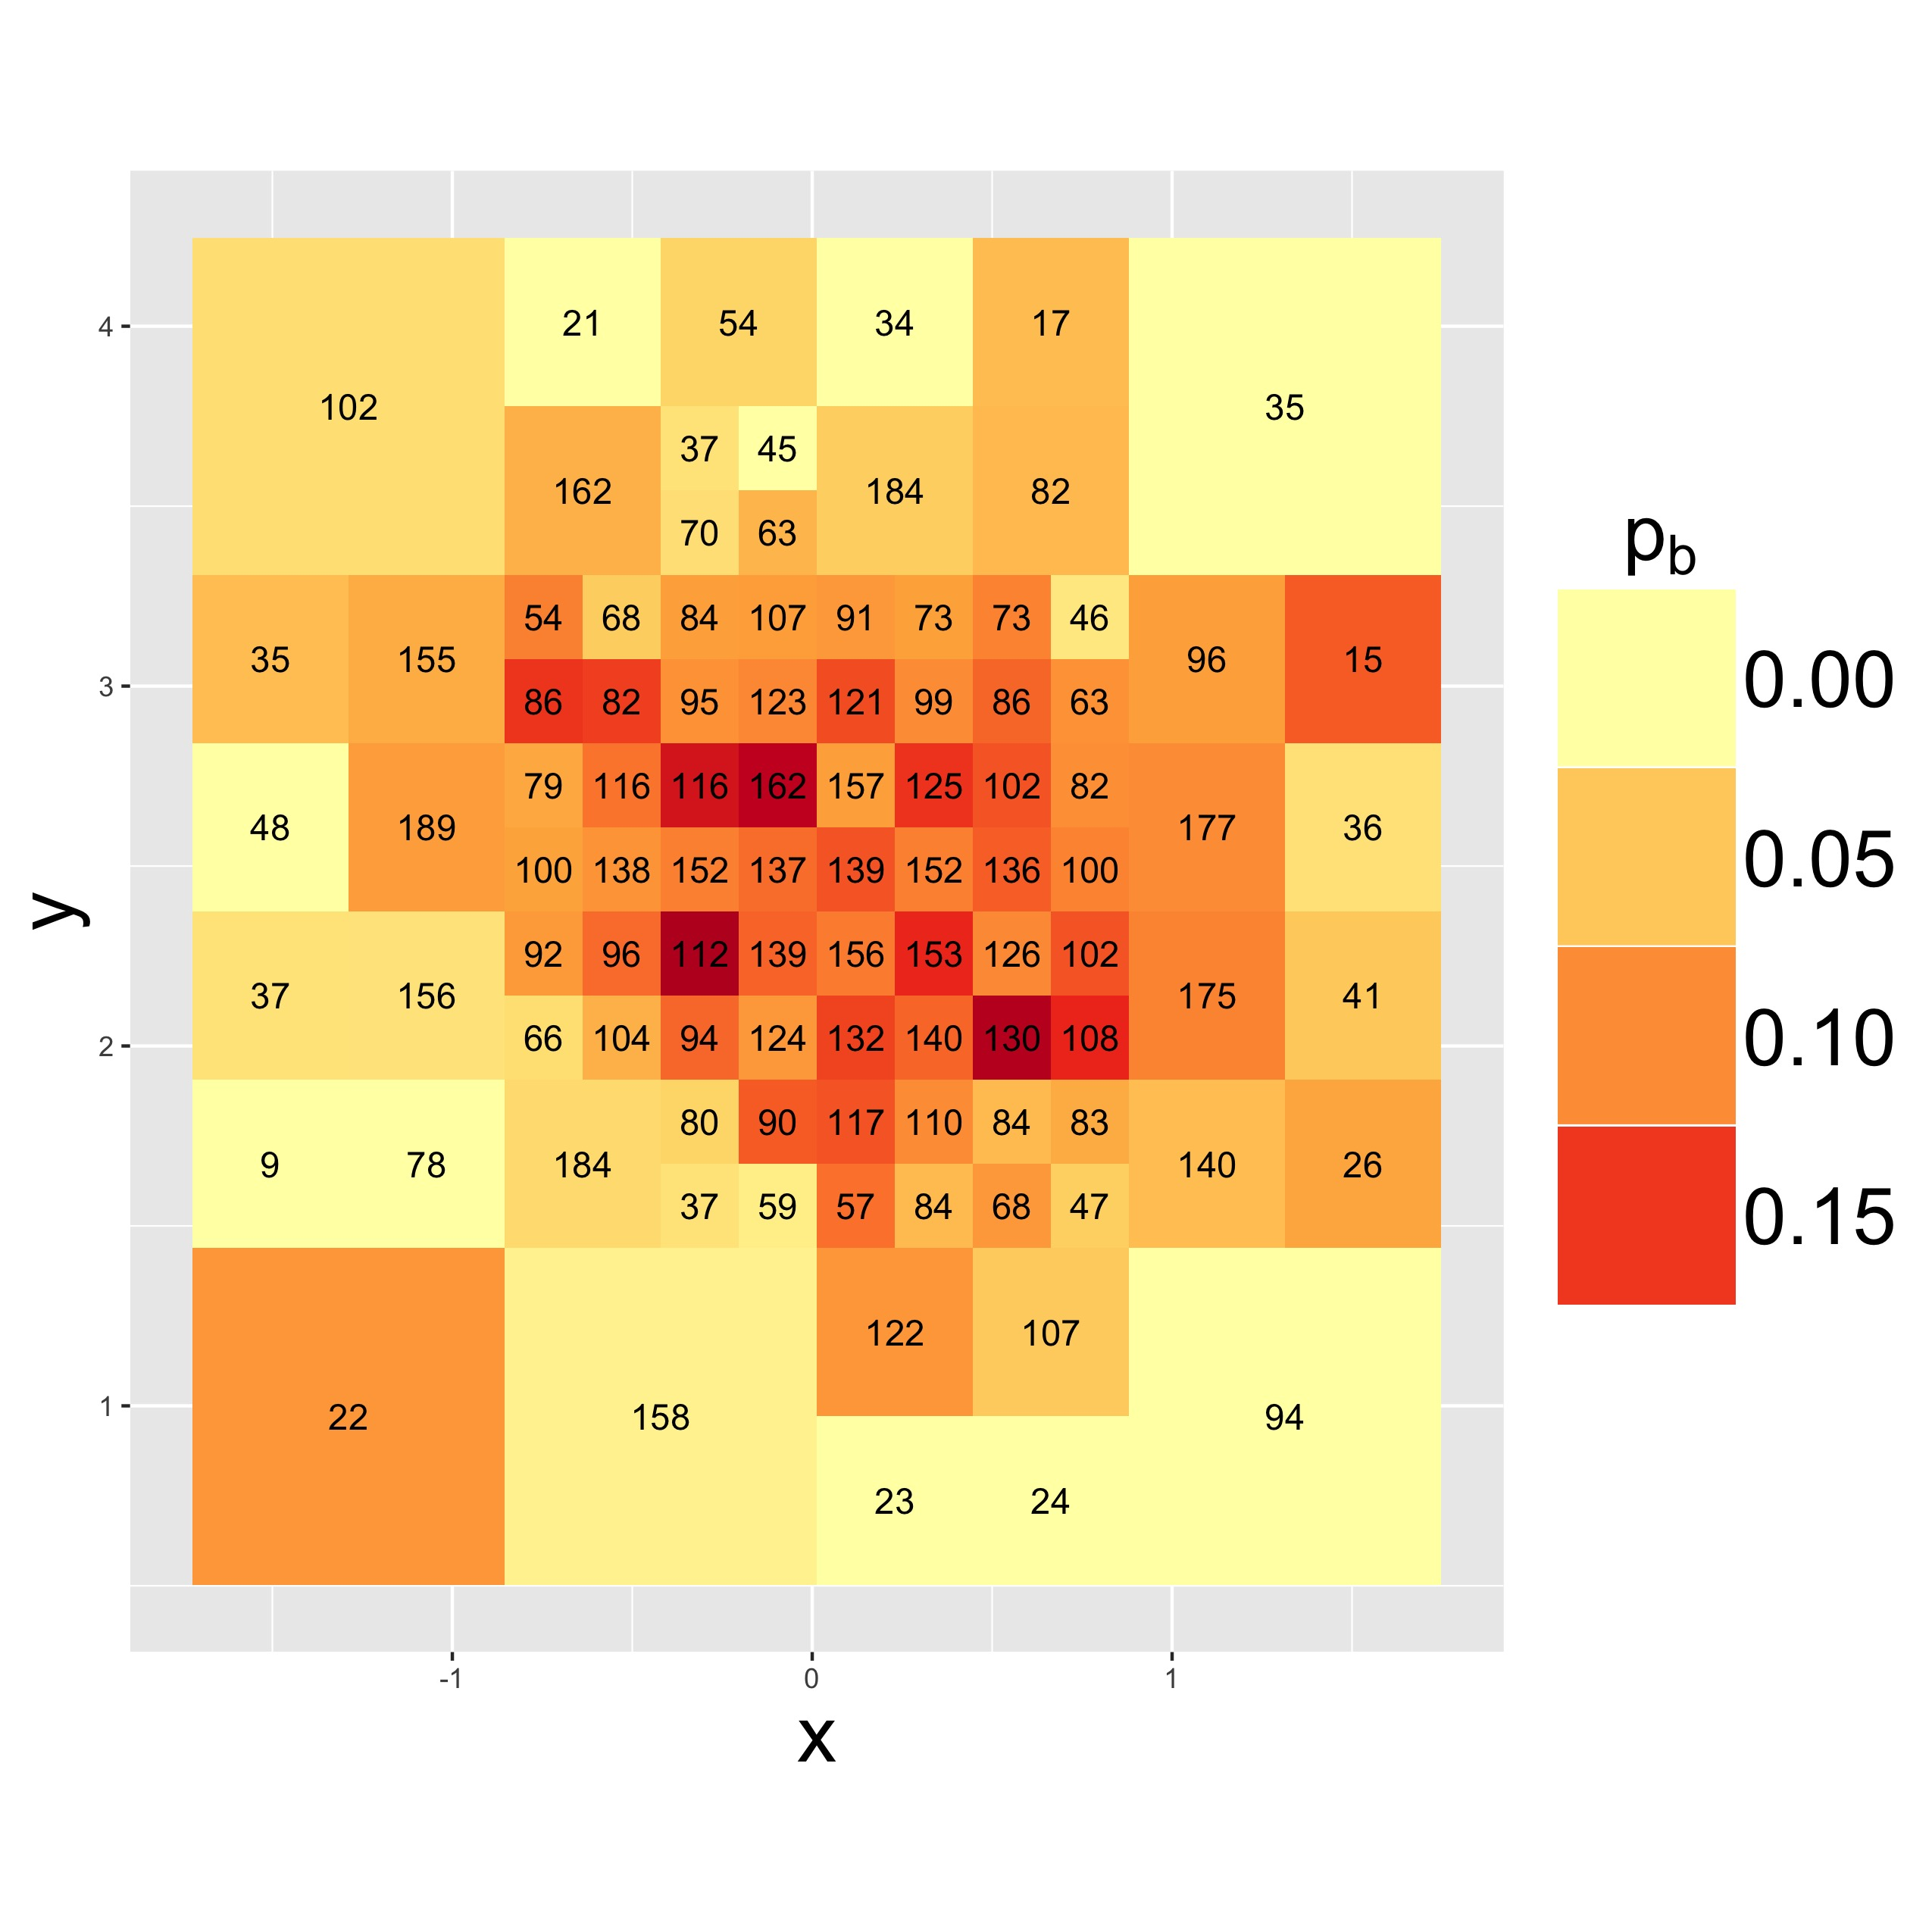
\includegraphics[scale=.08]{Images/Chapter16x16_200.jpg} 
      	\caption{Two iterations in the variable-resolution algorithm. The algorithm subdivides all boxes with a sample size (printed on box) greater than 200. This iteration yields the map on the right, from the map in the middle.}
      	\end{figure}
The new iteration yields the map on the right from the middle map. The new map consists of 97 boxes, with a mean box sample size of 94.57, and median of 94. Box 9 contains the fewest observations, and box 189 contains the most. Box 63 serves as the first quartile, while box 125 serves as the third quartile. 

Figure \ref{fig:allvr} shows the VR heat map for every iteration, for stopping rule $n_{b} < 200$.
        \begin{figure}[H]
      	\centering
      	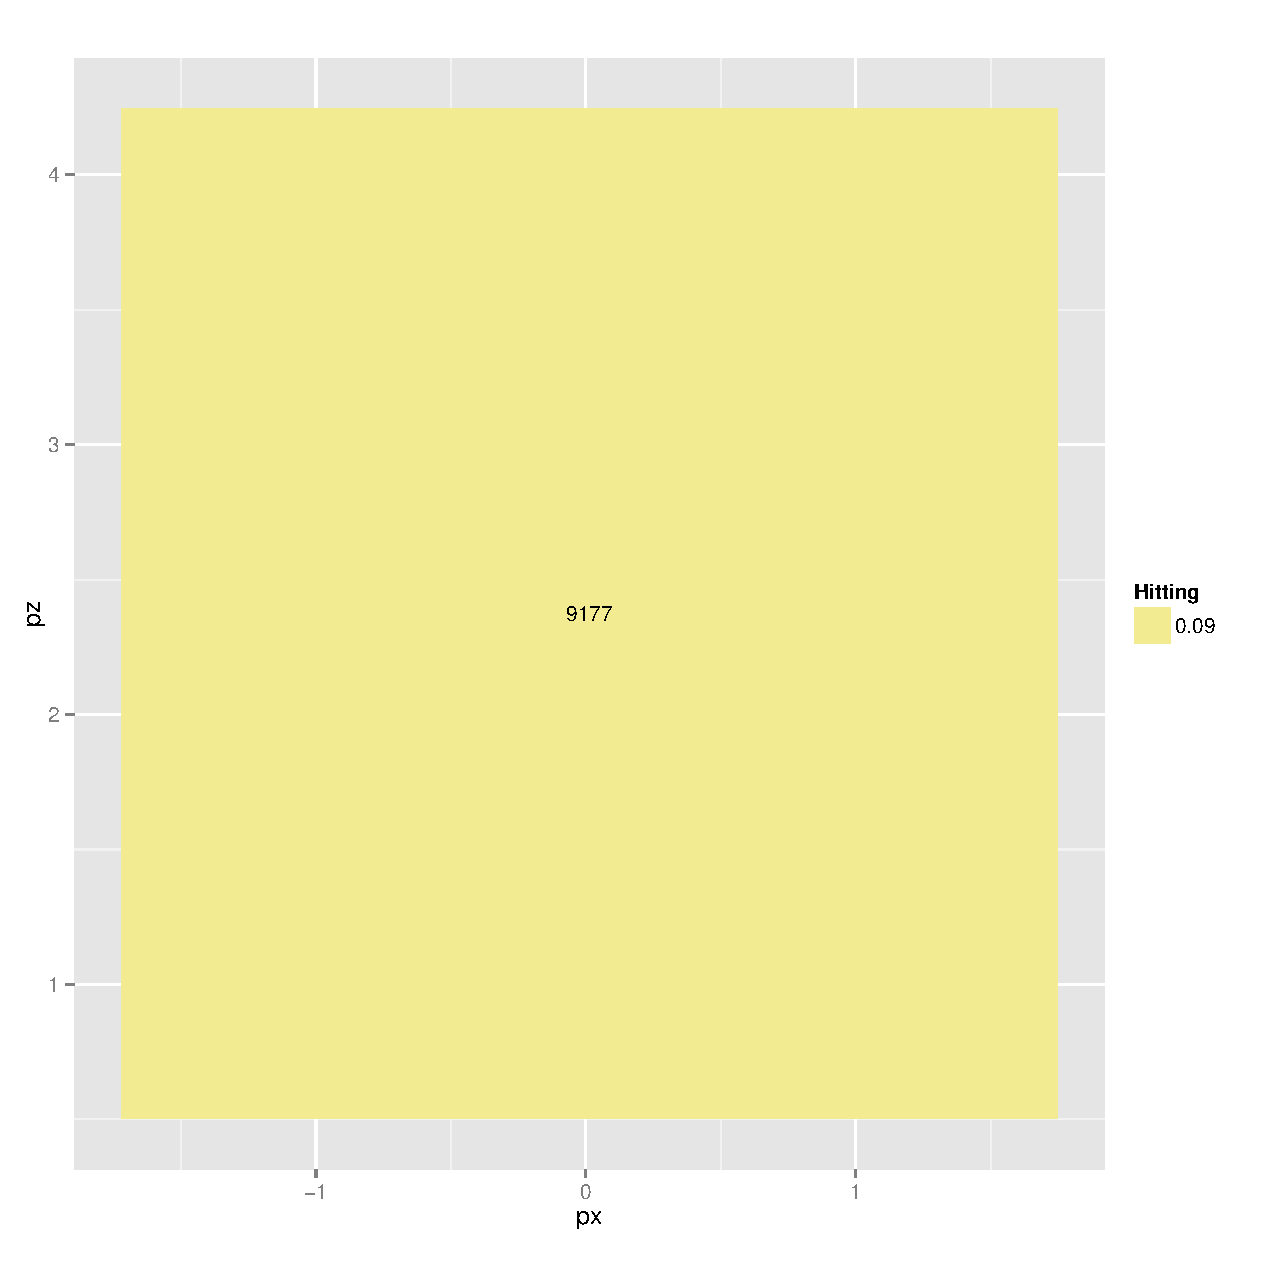
\includegraphics[scale=0.05]{Images/Chapter1x1.jpg}
      	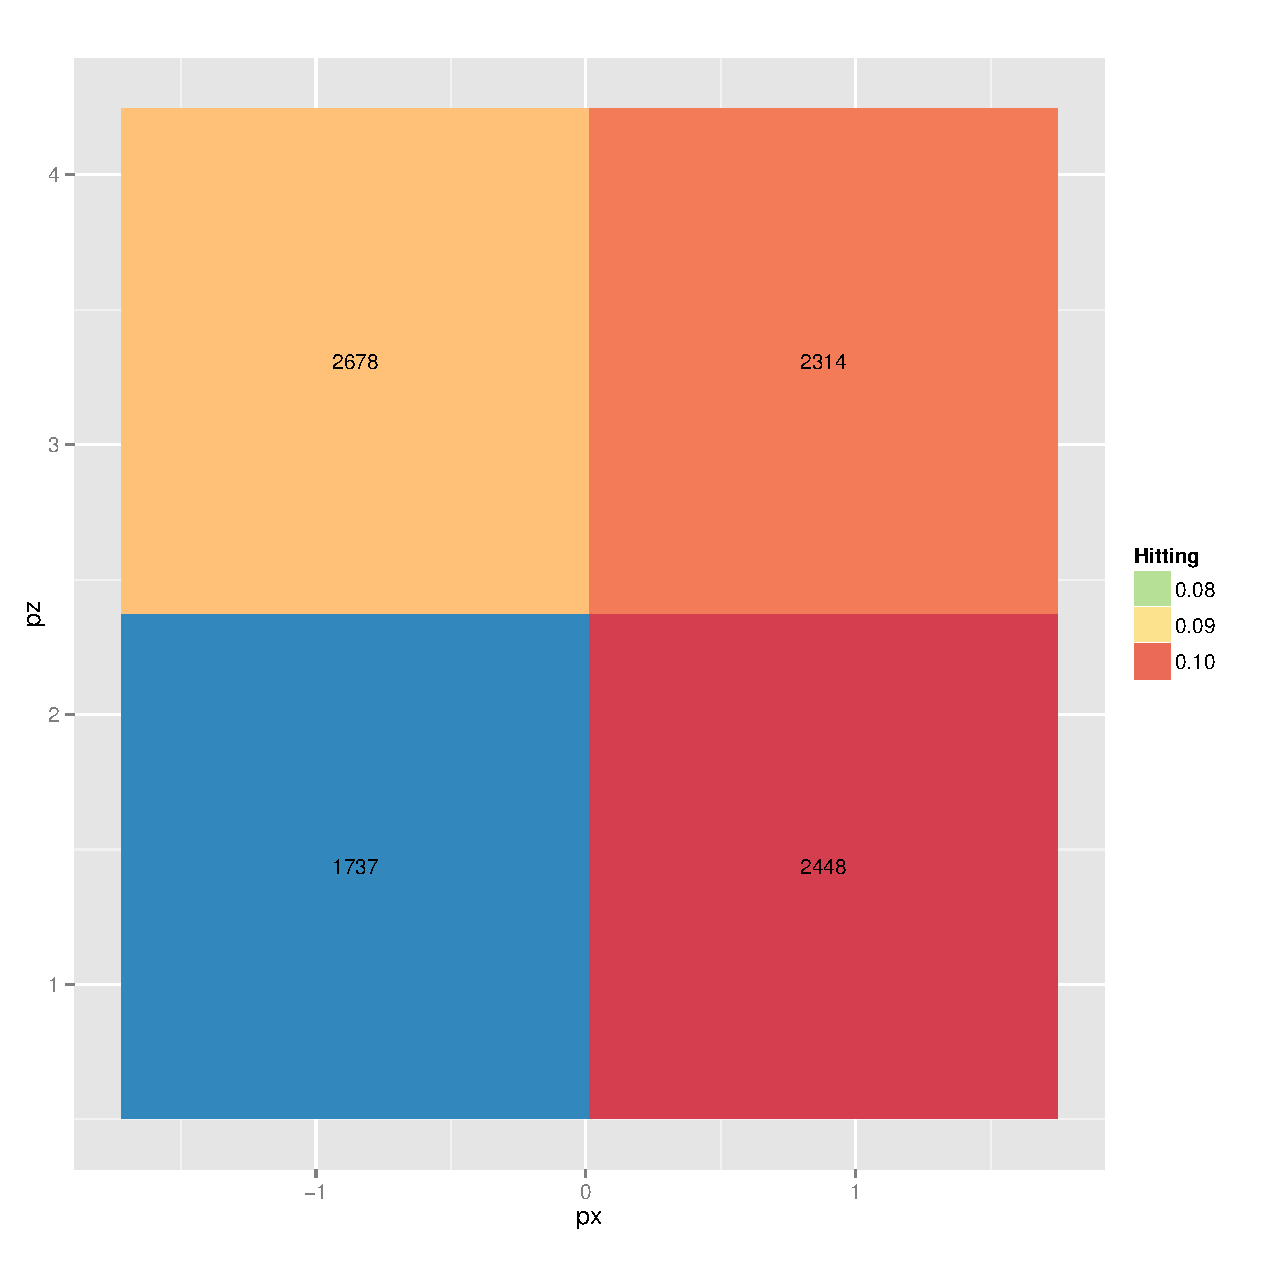
\includegraphics[scale=0.05]{Images/Chapter2x2.jpg}
      	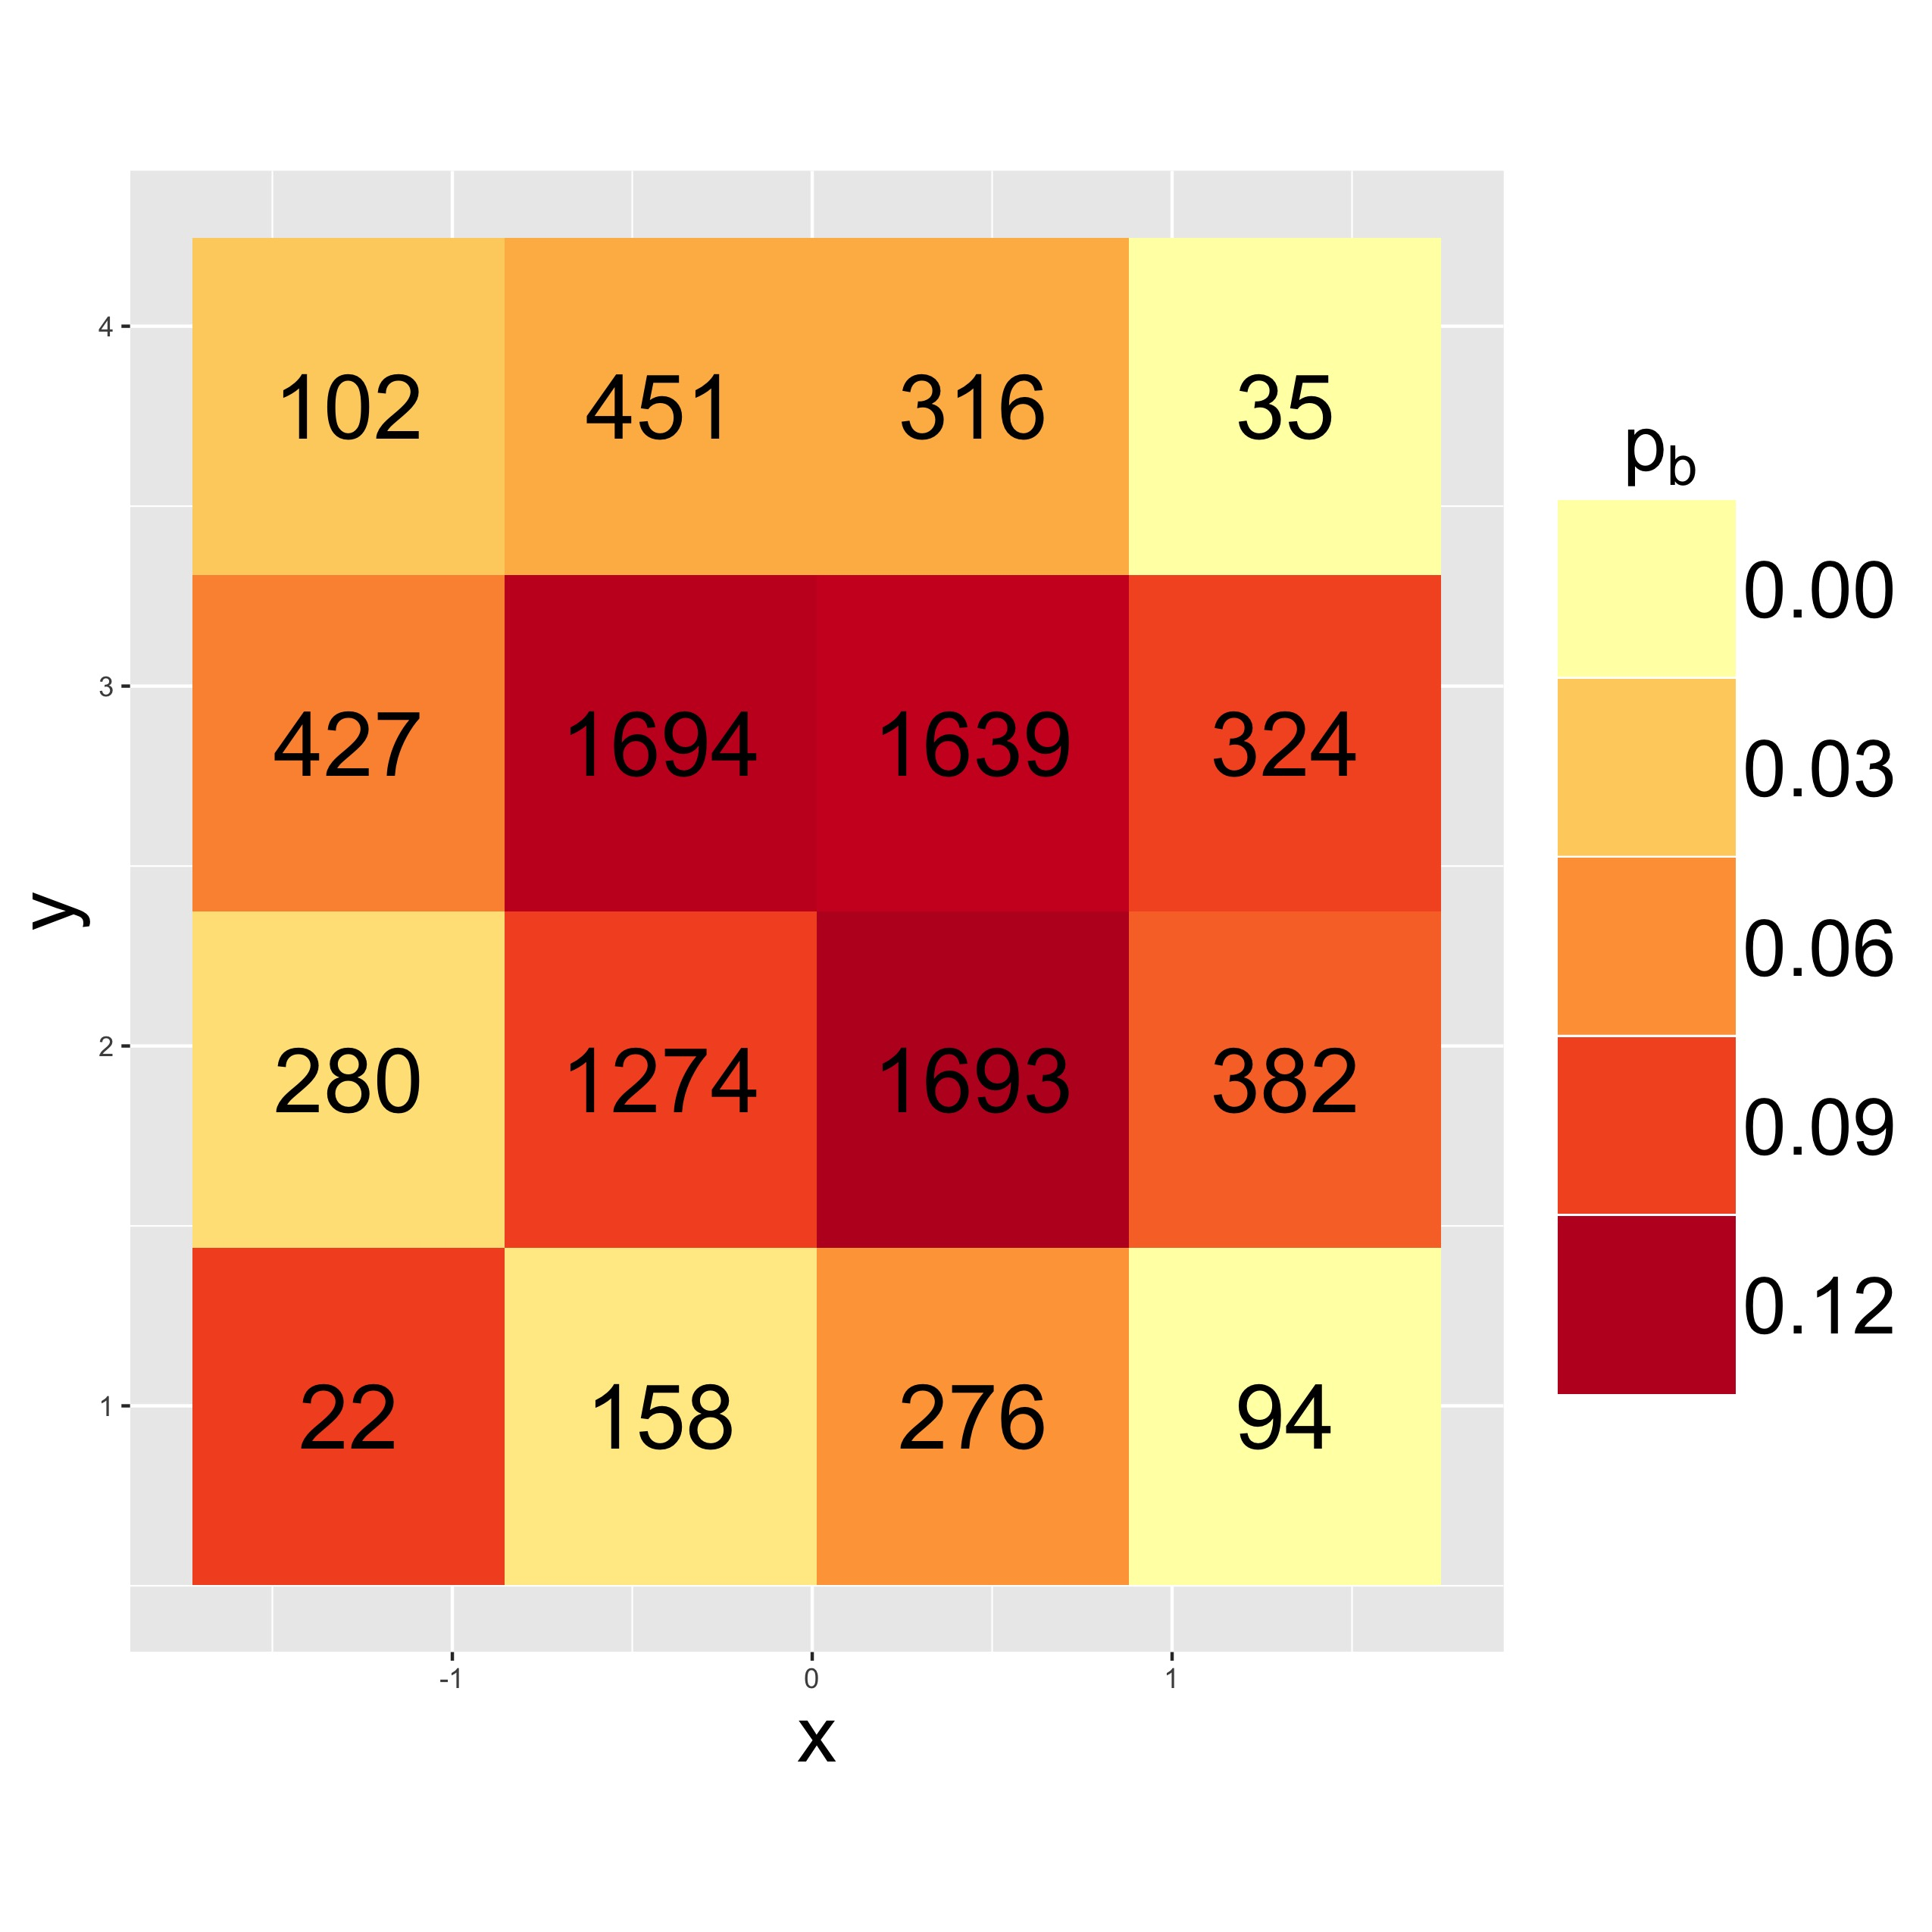
\includegraphics[scale=0.05]{Images/Chapter4x4.jpg}
      	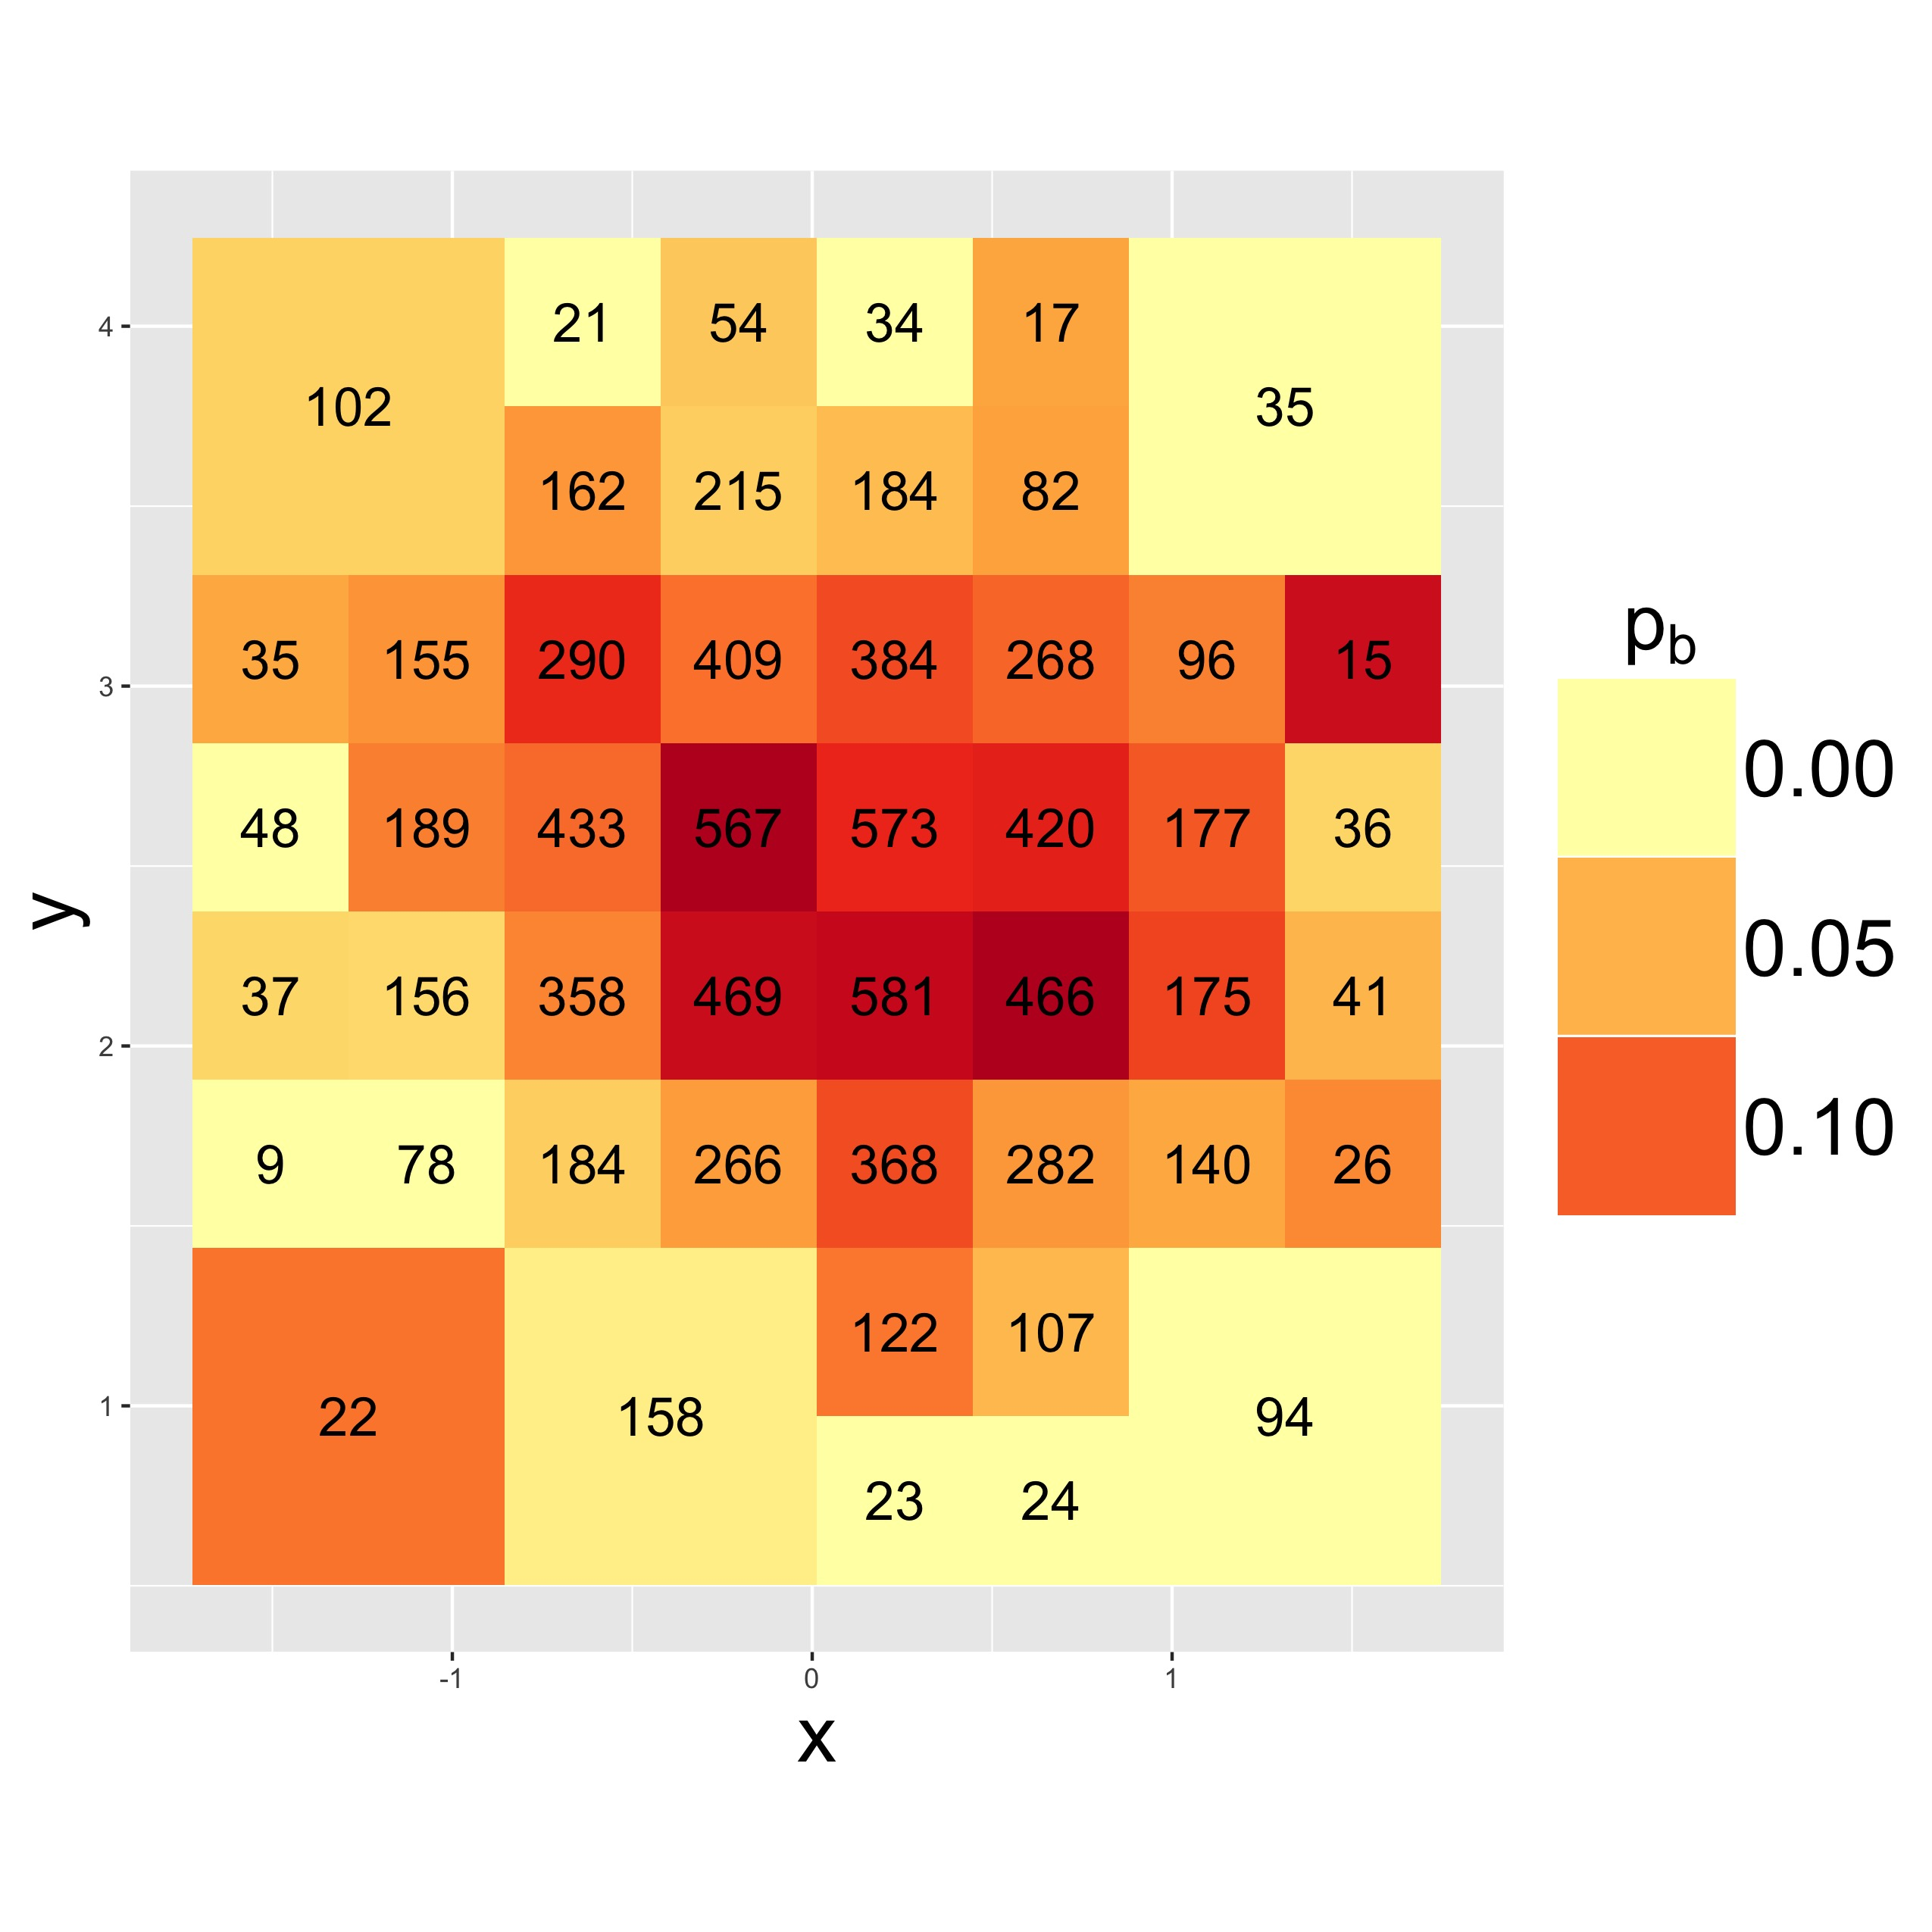
\includegraphics[scale=0.05]{Images/Chapter8x8_200.jpg} 
      	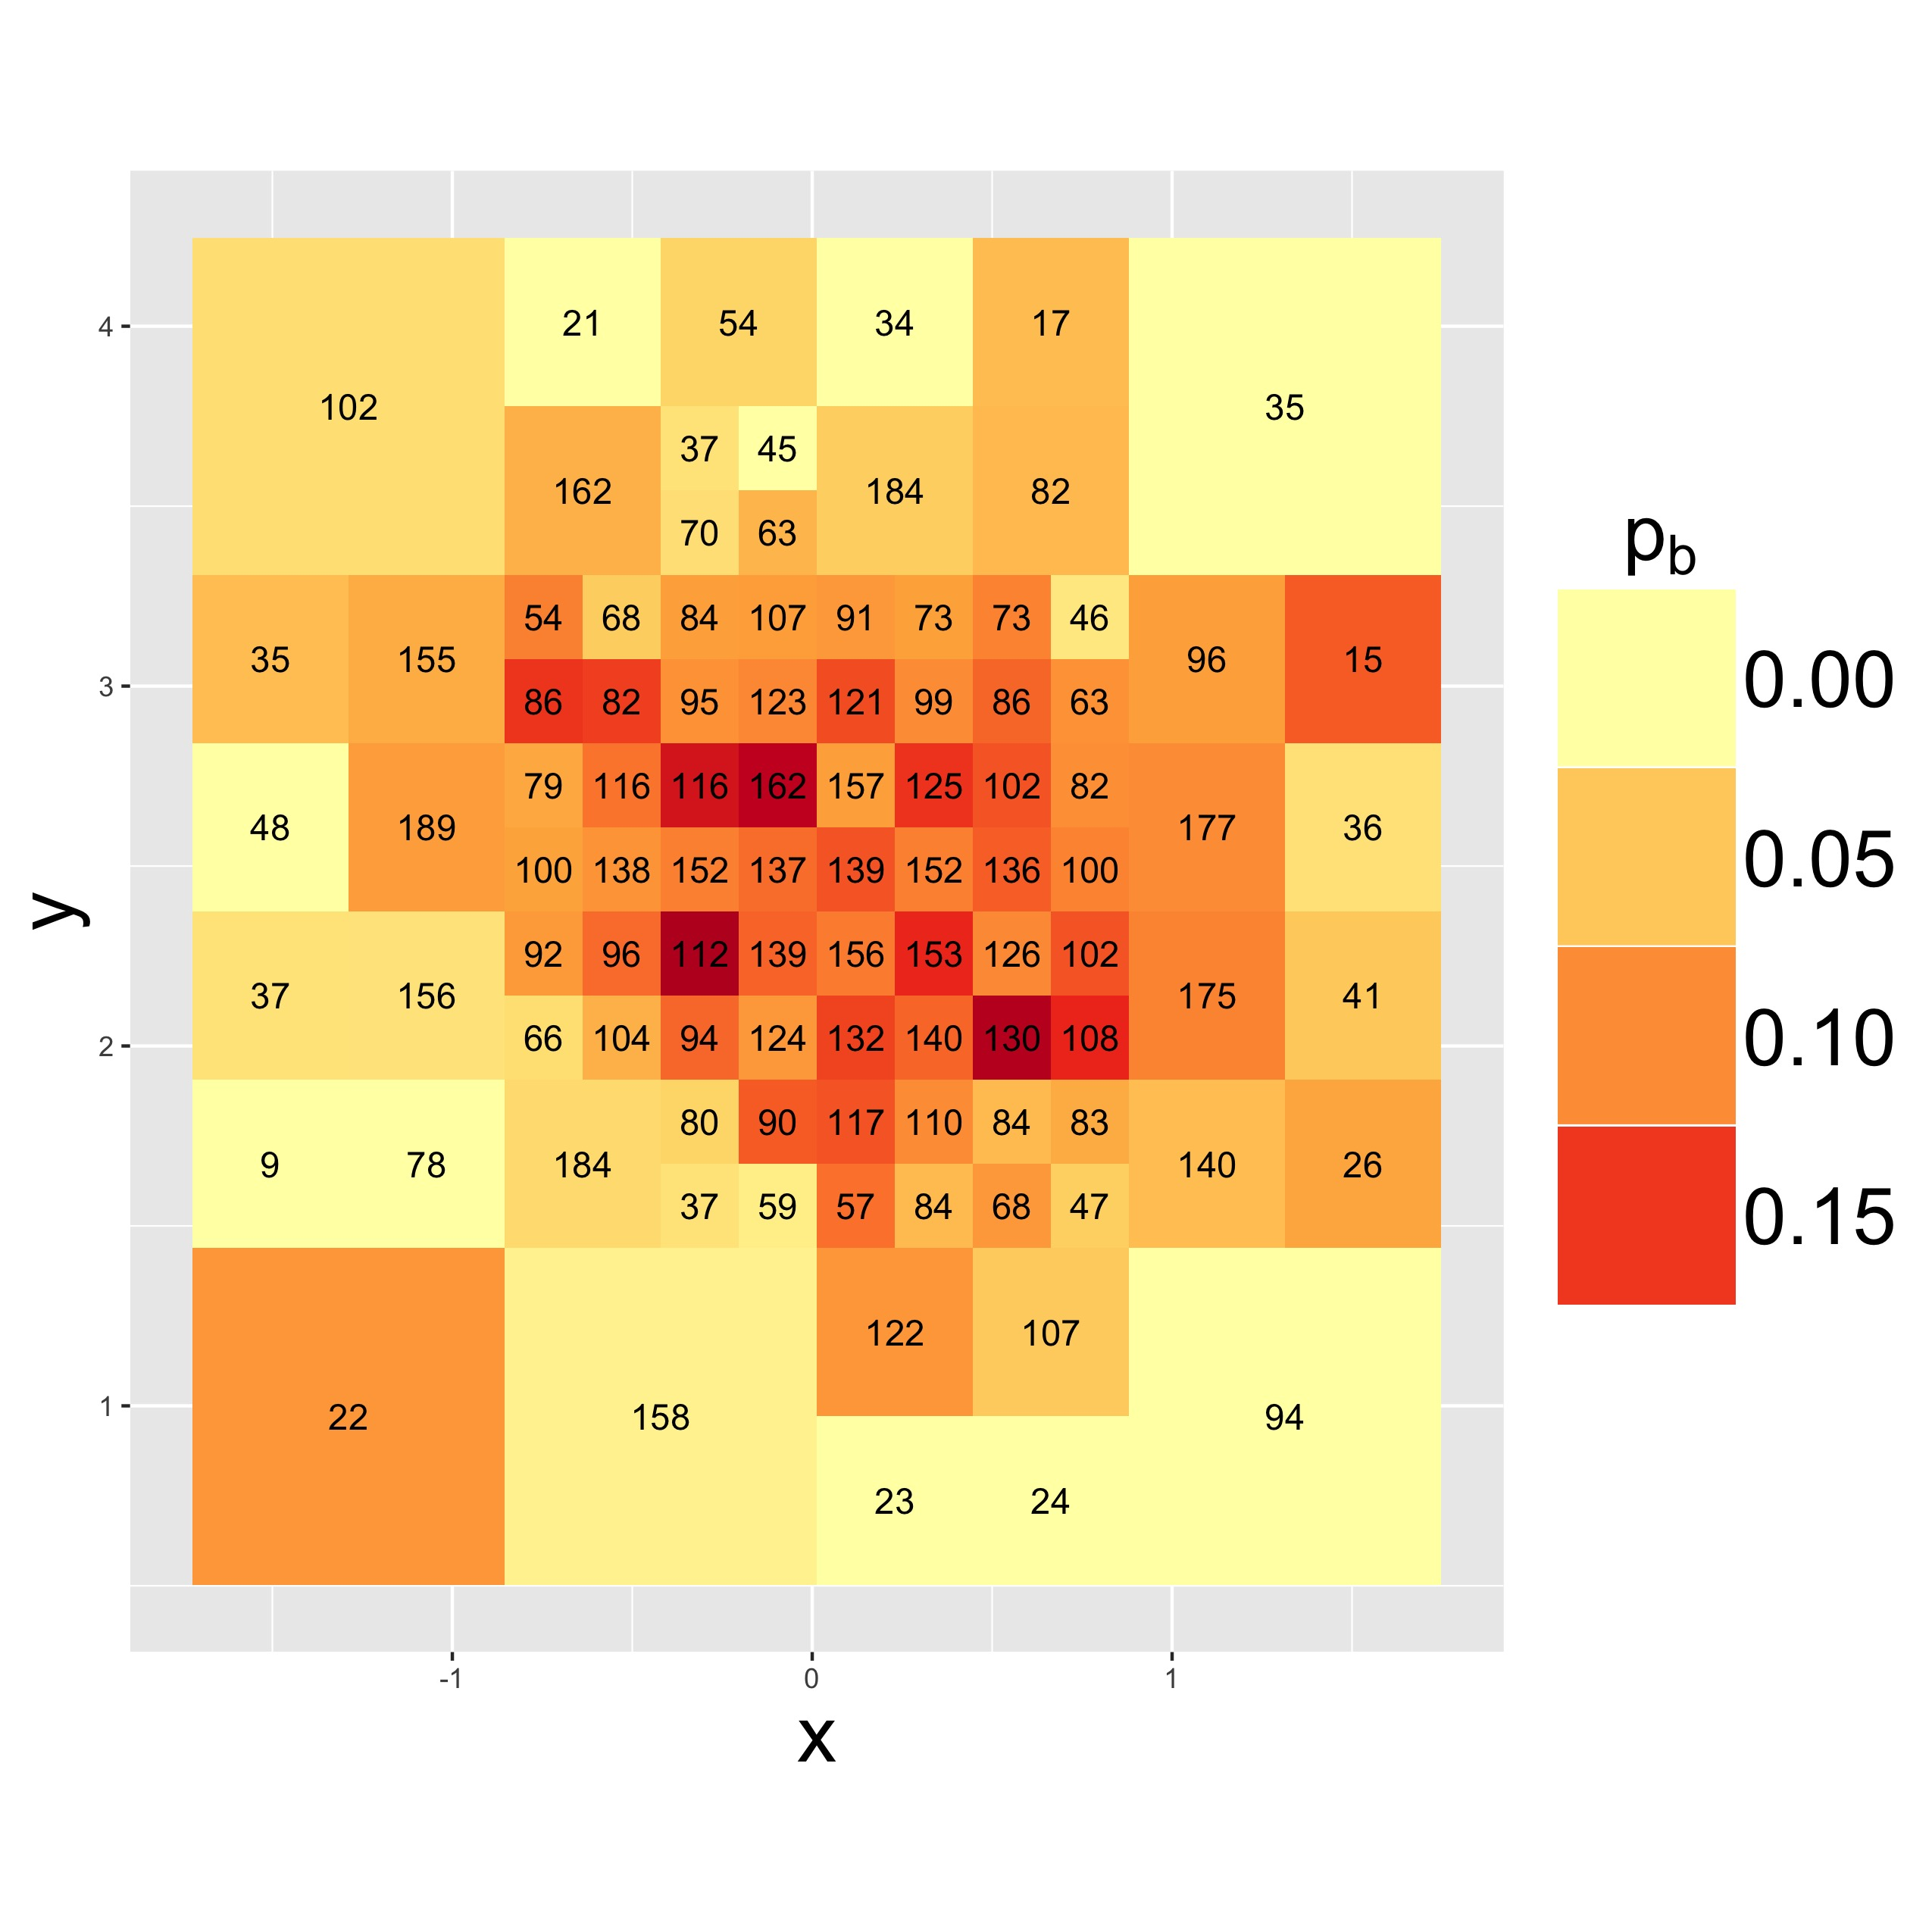
\includegraphics[scale=0.05]{Images/Chapter16x16_200.jpg} 
      	\caption{Variable-resolution heat map sequence. Starting from the top left, the algorithm subdivides all boxes with a sample size (printed on box) greater than 200. The maps convey Jhonny Peralta's empirical success probability by mapping $\hat{p}_{b}$ to a color.}
      	\label{fig:allvr}
      	\end{figure}
      	
\subsection{Data Density Information}

In VR heat maps, regions of greater observation density have smaller boxes, and thus more spatially specific estimates. In this way the size of the box conveys density information, which heat maps typically conceal. This new feature derives from the fact that box subdivisions persist until box sample sizes drop below 200 (in this map). Figure \ref{fig:density} demonstrates the correspondence between observation density and box size, by comparing a scatterplot to a VR heat map. 
        \begin{figure}[H]
      	\centering
      	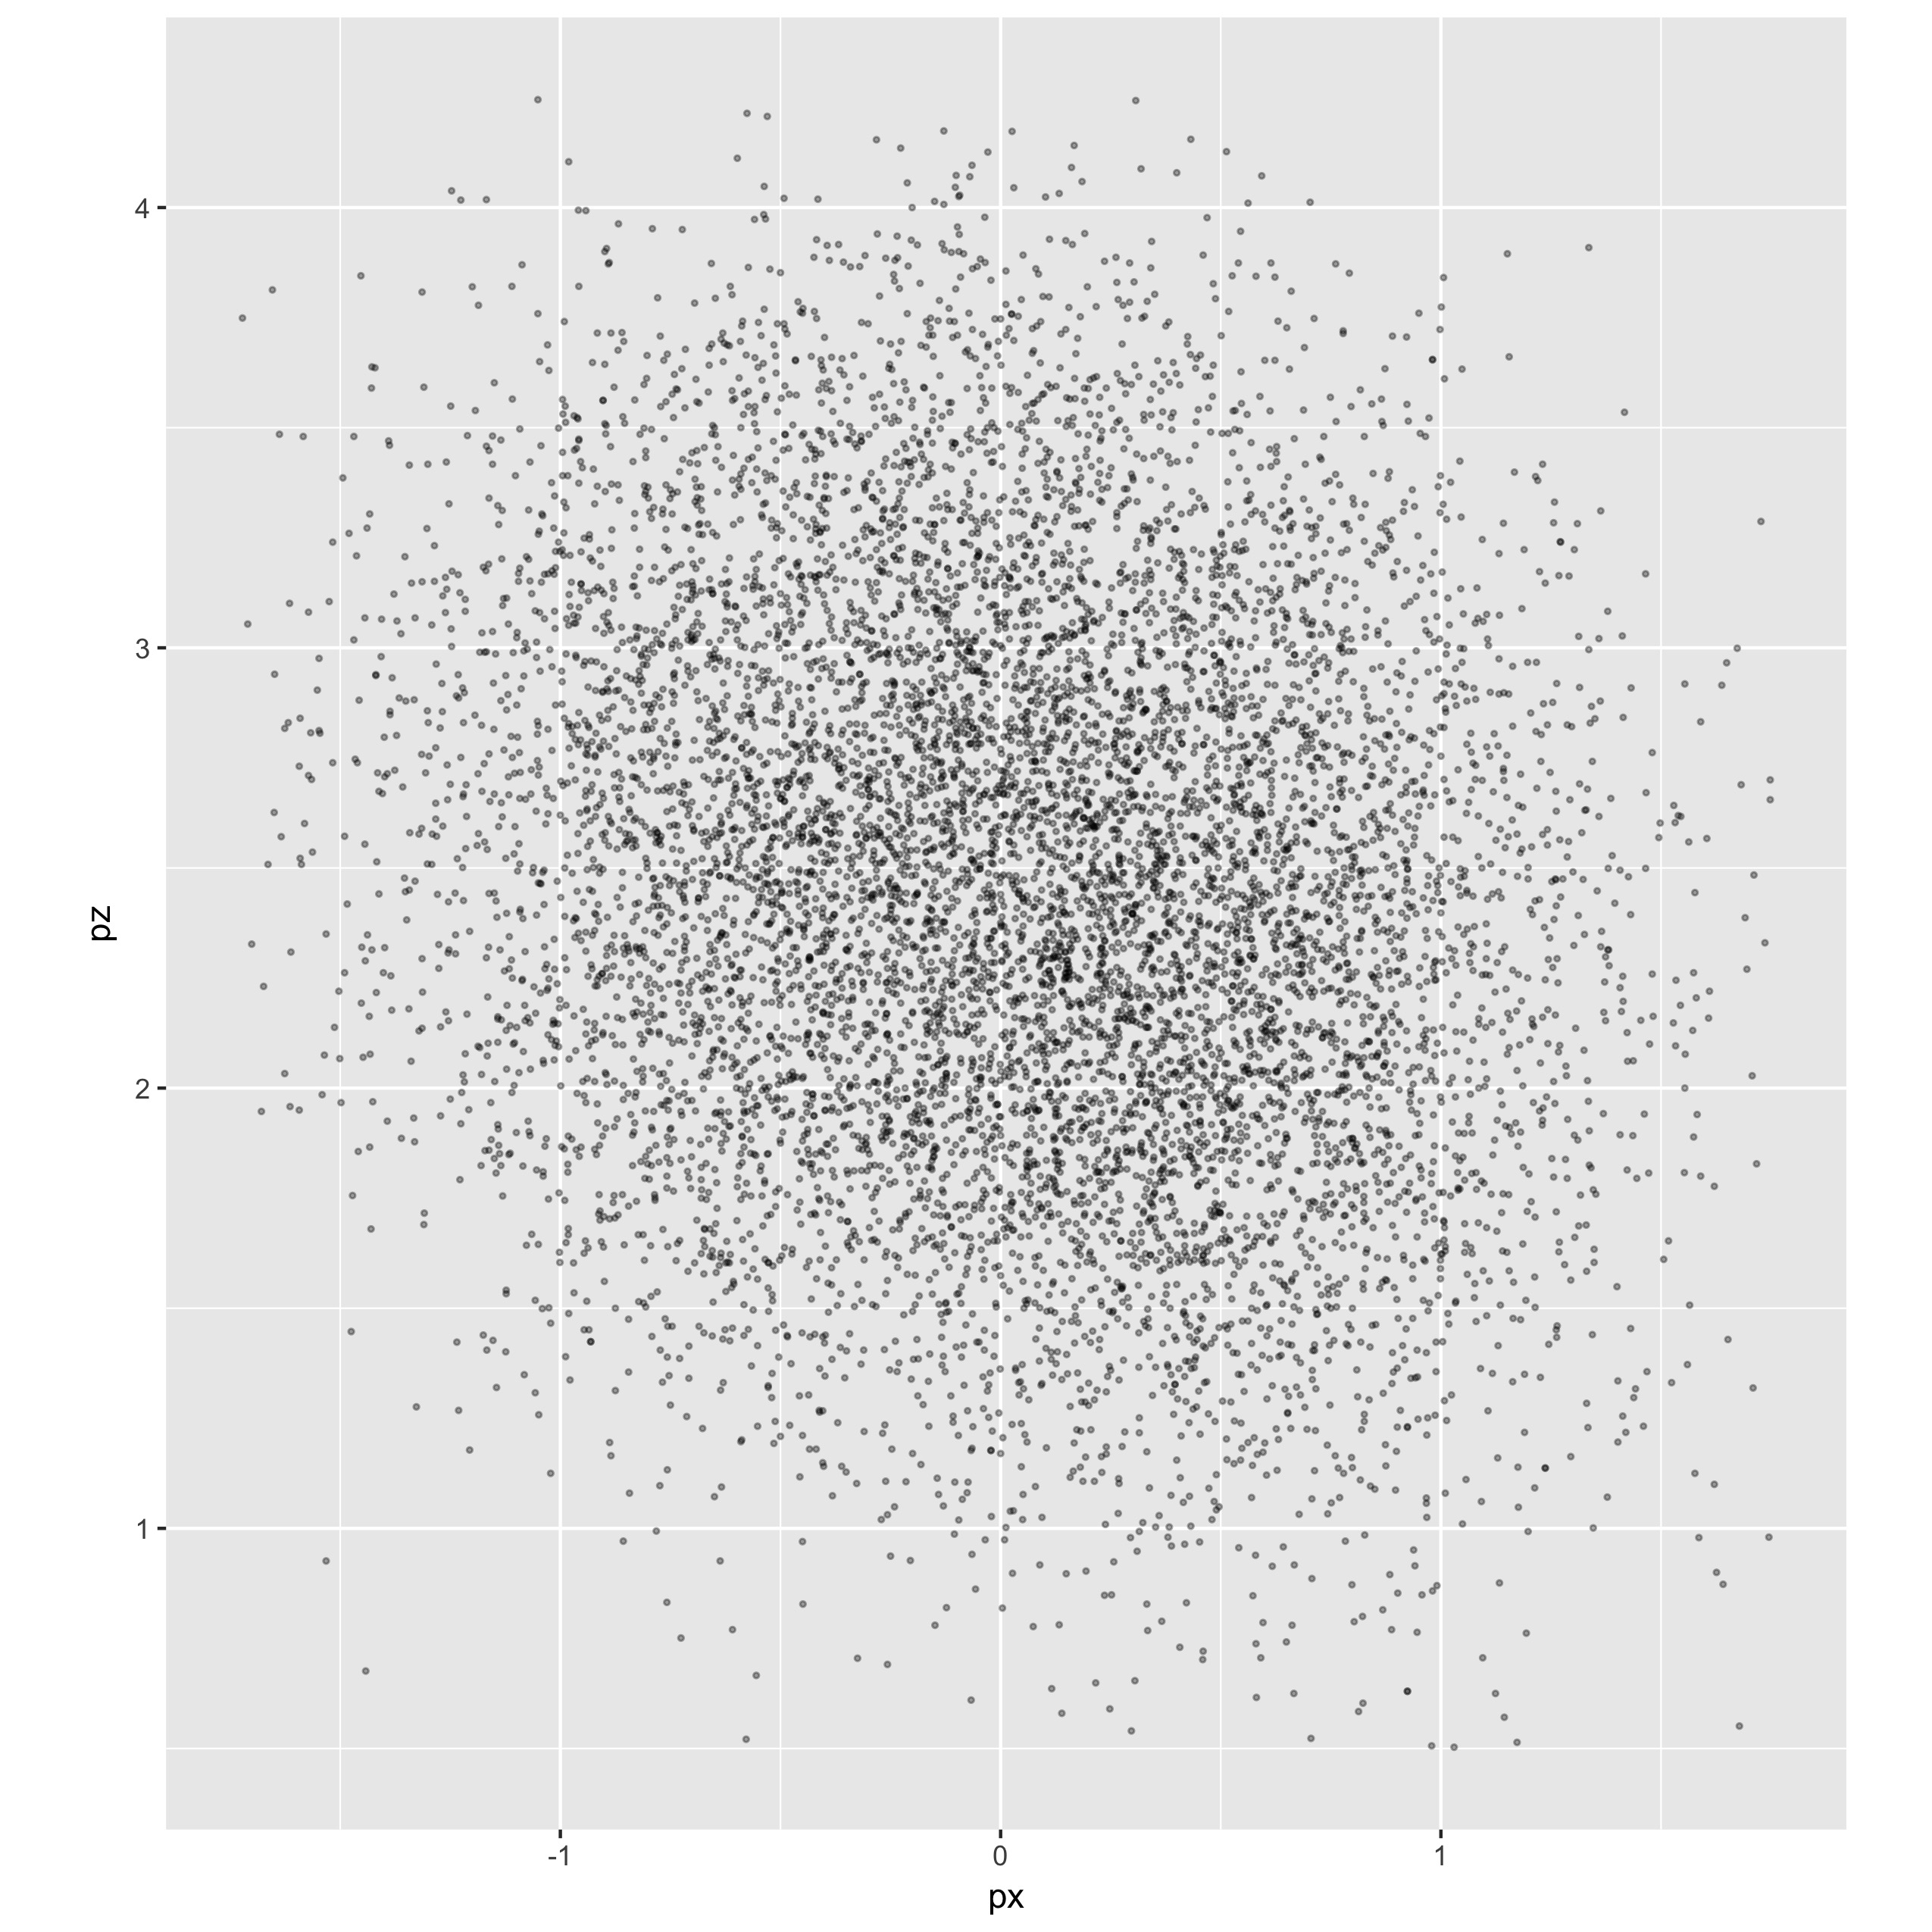
\includegraphics[scale=.07]{Images/density.jpg}
      	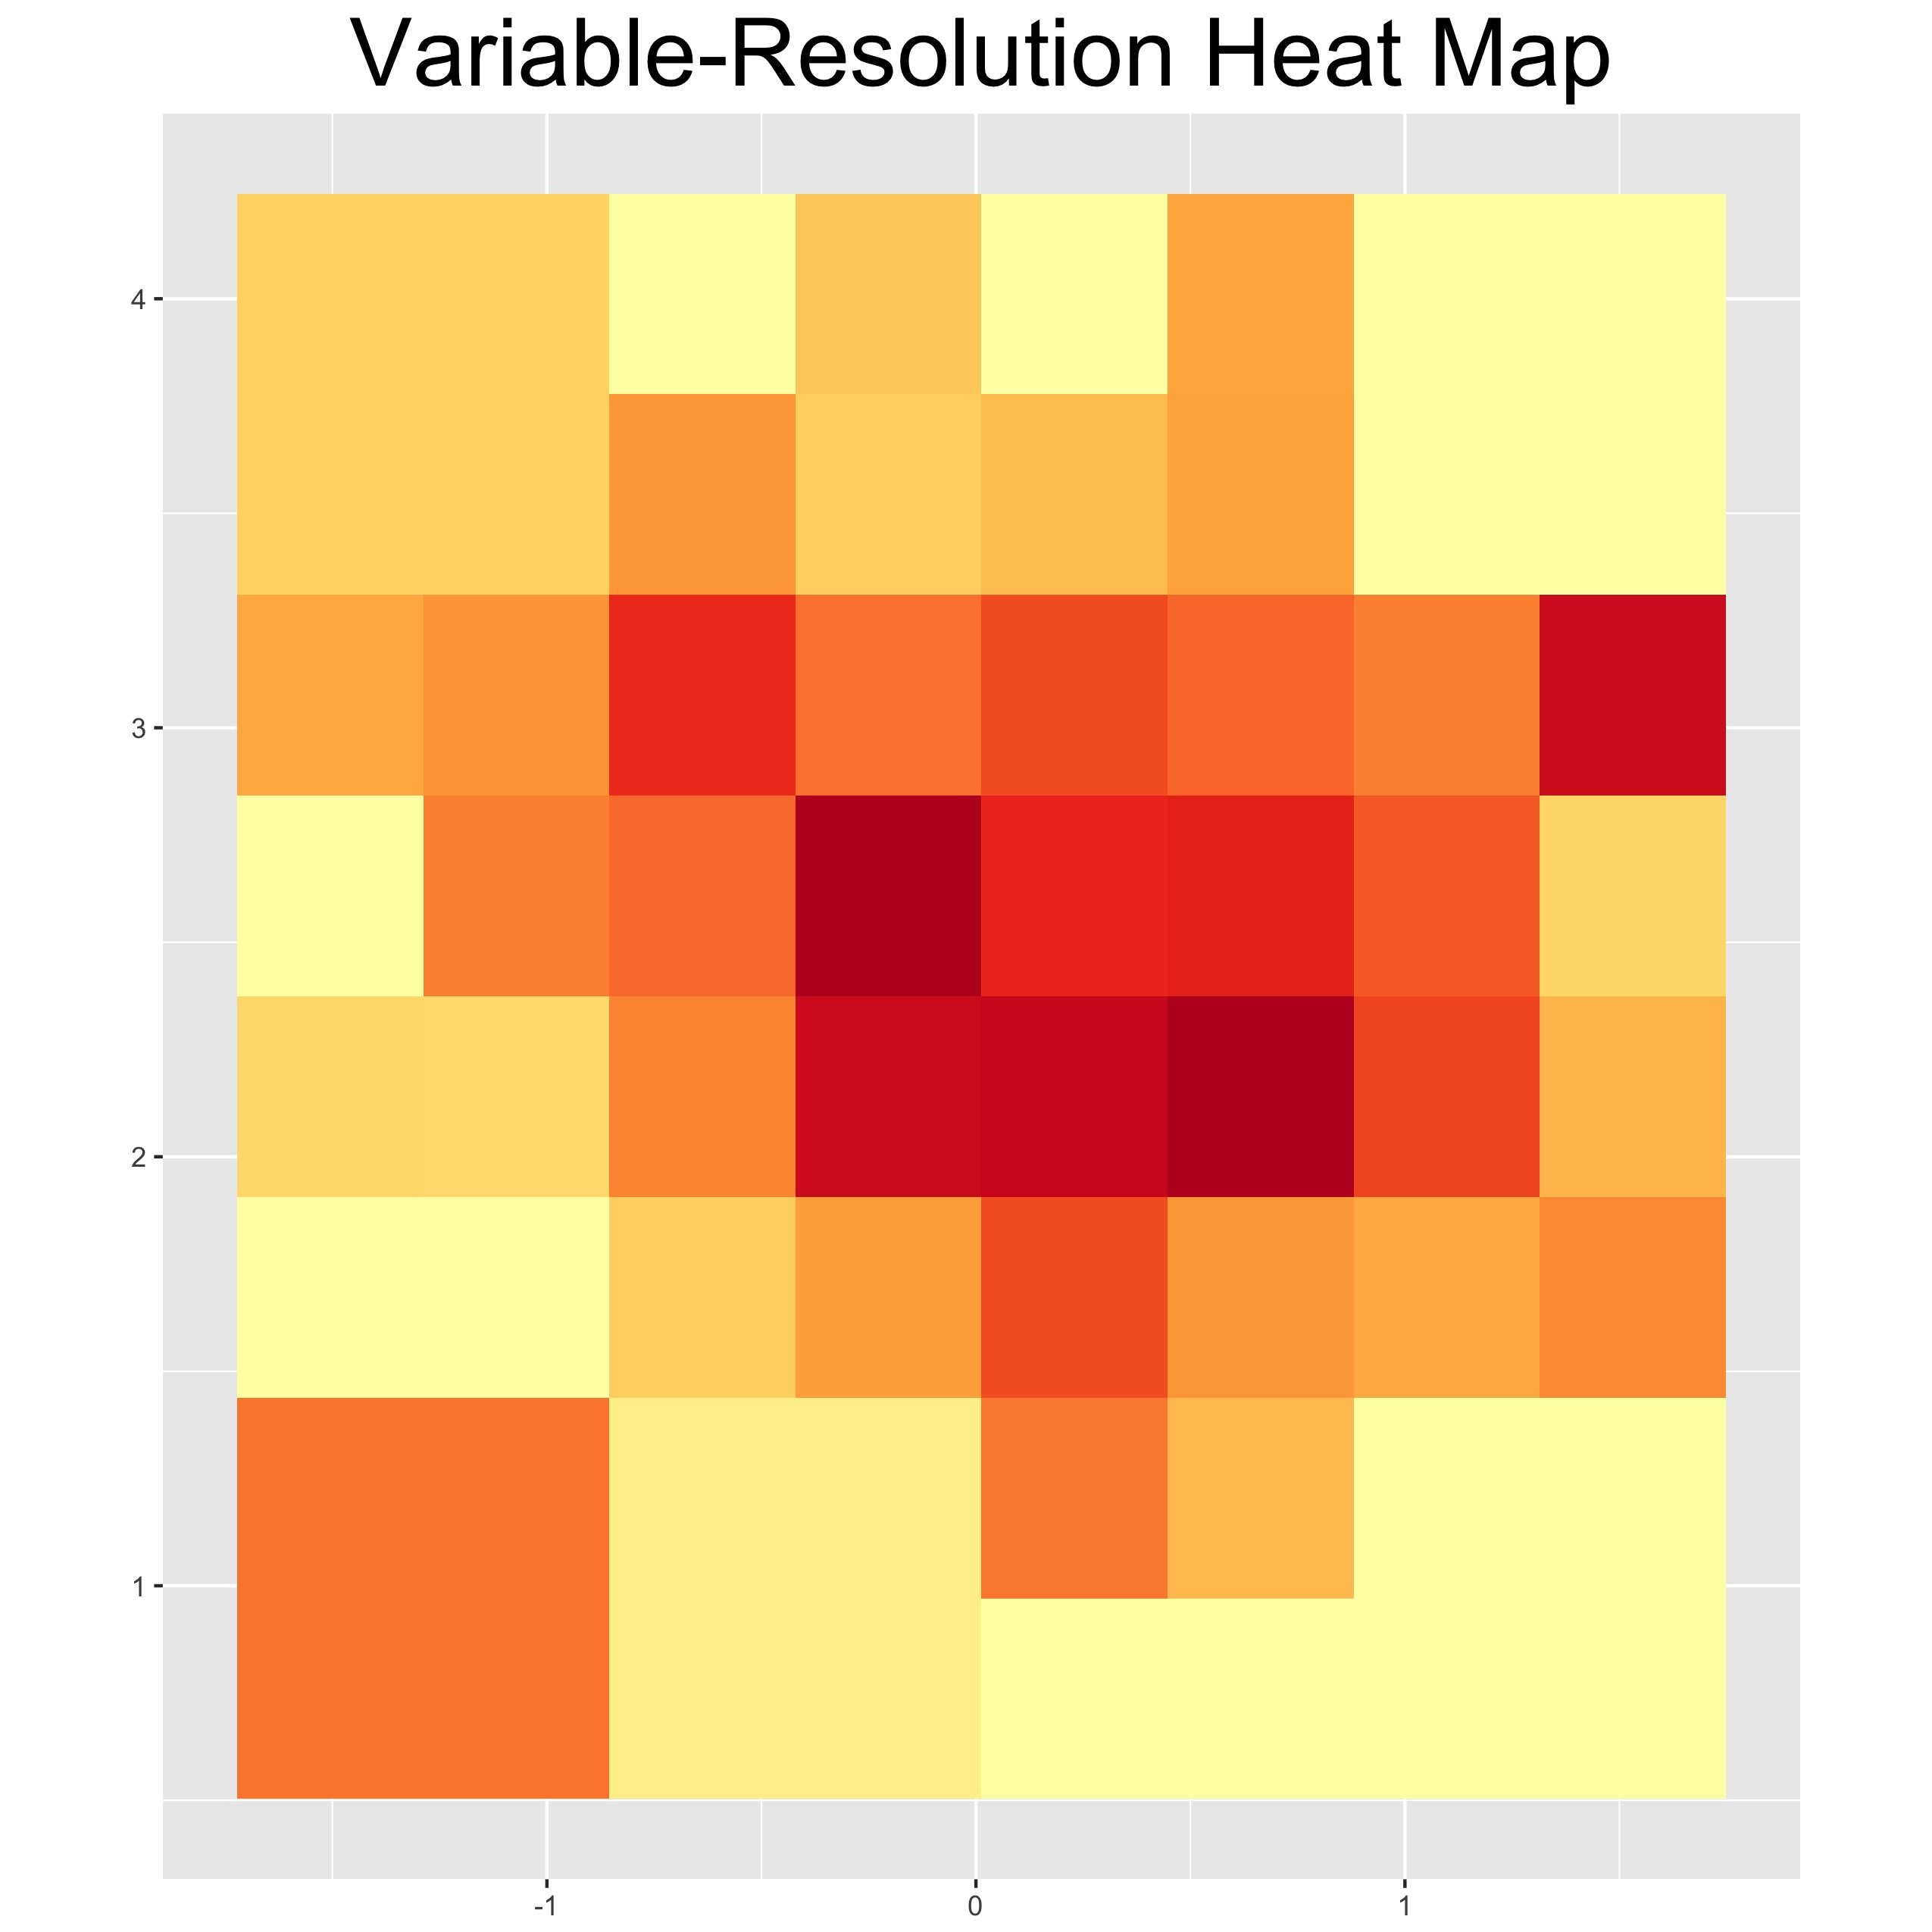
\includegraphics[scale=.07]{Images/density_comp.jpg} 
      	\caption{Variable-resolution (VR) heat maps convey data density. Comparing Jhonny Peralta's scatter plot and VR heat map shows the correspondence between data density and box size. The finer resolution regions in the heat map correspond to greater data density, whereas bigger boxes indicate lower density. Traditional heat maps omit this information.}
      	\label{fig:density}
      	\end{figure}
Notice how smaller boxes correspond to higher data density, while larger boxes indicate lower density. This contrasts favorably to traditional heat maps, where uniform resolution conceals data density. VR heat maps convey valuable, previously omitted, data density information to the viewer. 
      	
\subsection{Example: Alternate Stopping Rule} % ===================
      	
In this section we apply the VR algorithm to the same data, but with stopping rule $n_{b} < 100$ instead of $n_{b} < 200$. A comparison with the previous VR maps shows how the algorithm's iterations and outcome change with a different stopping rule. Figure \ref{fig:altsr} shows heat maps for all six VR iterations.
        \begin{figure}[H]
      	\centering
      	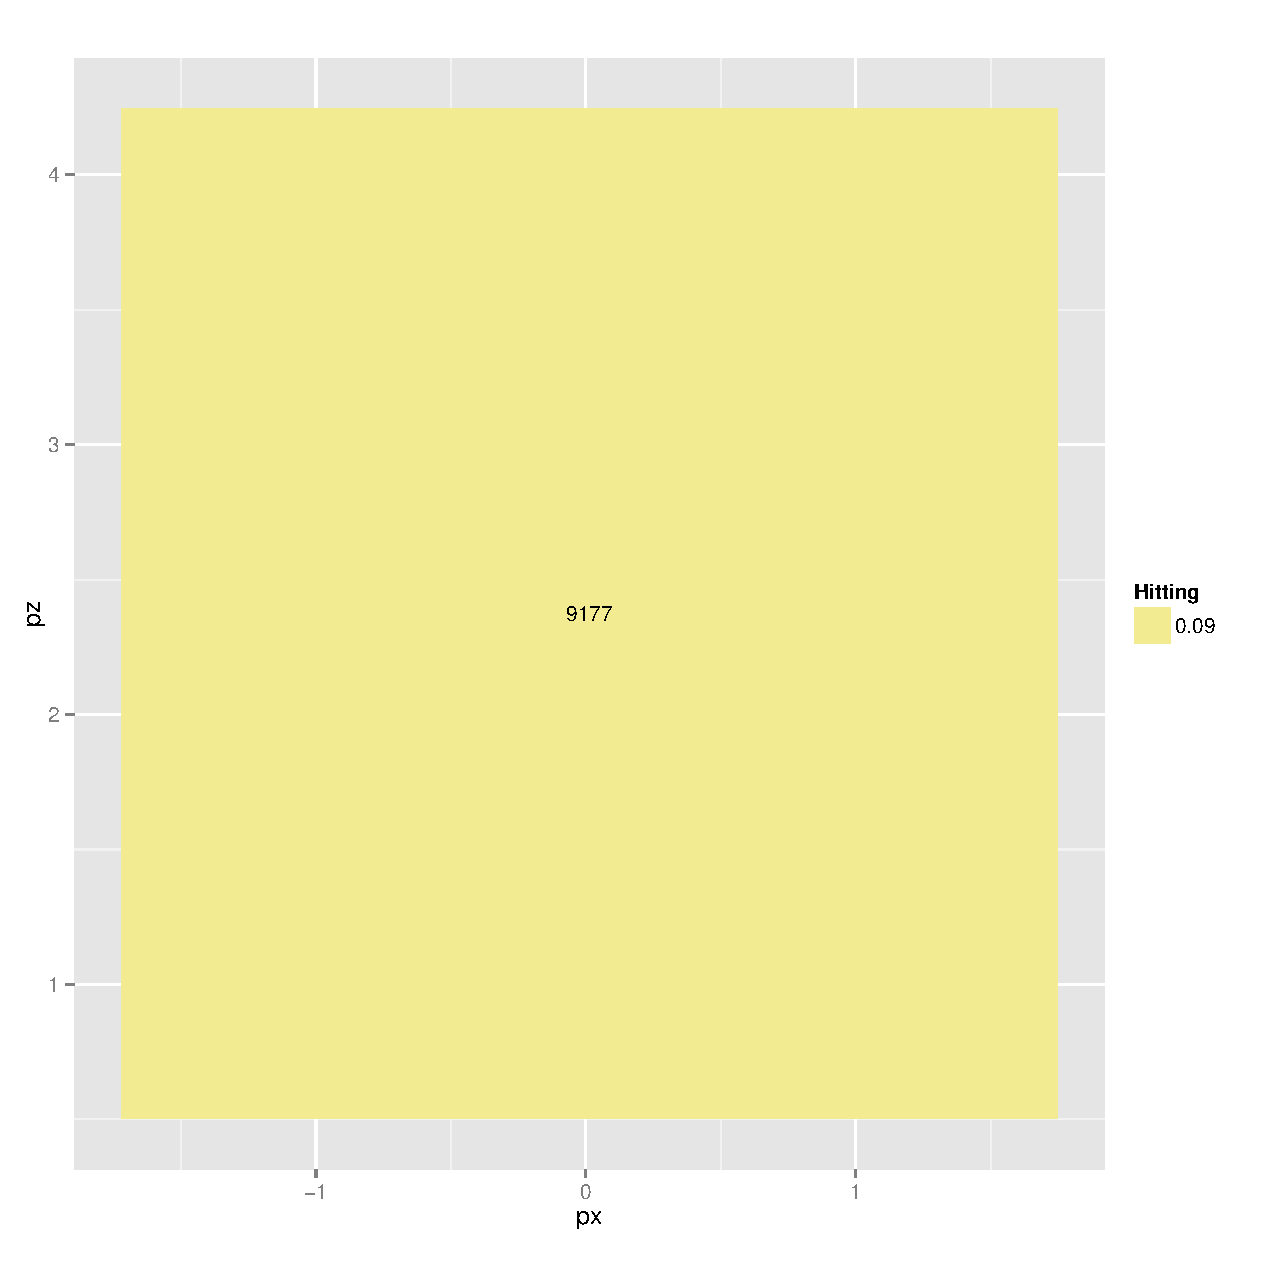
\includegraphics[scale=.05]{Images/Chapter1x1.jpg}
      	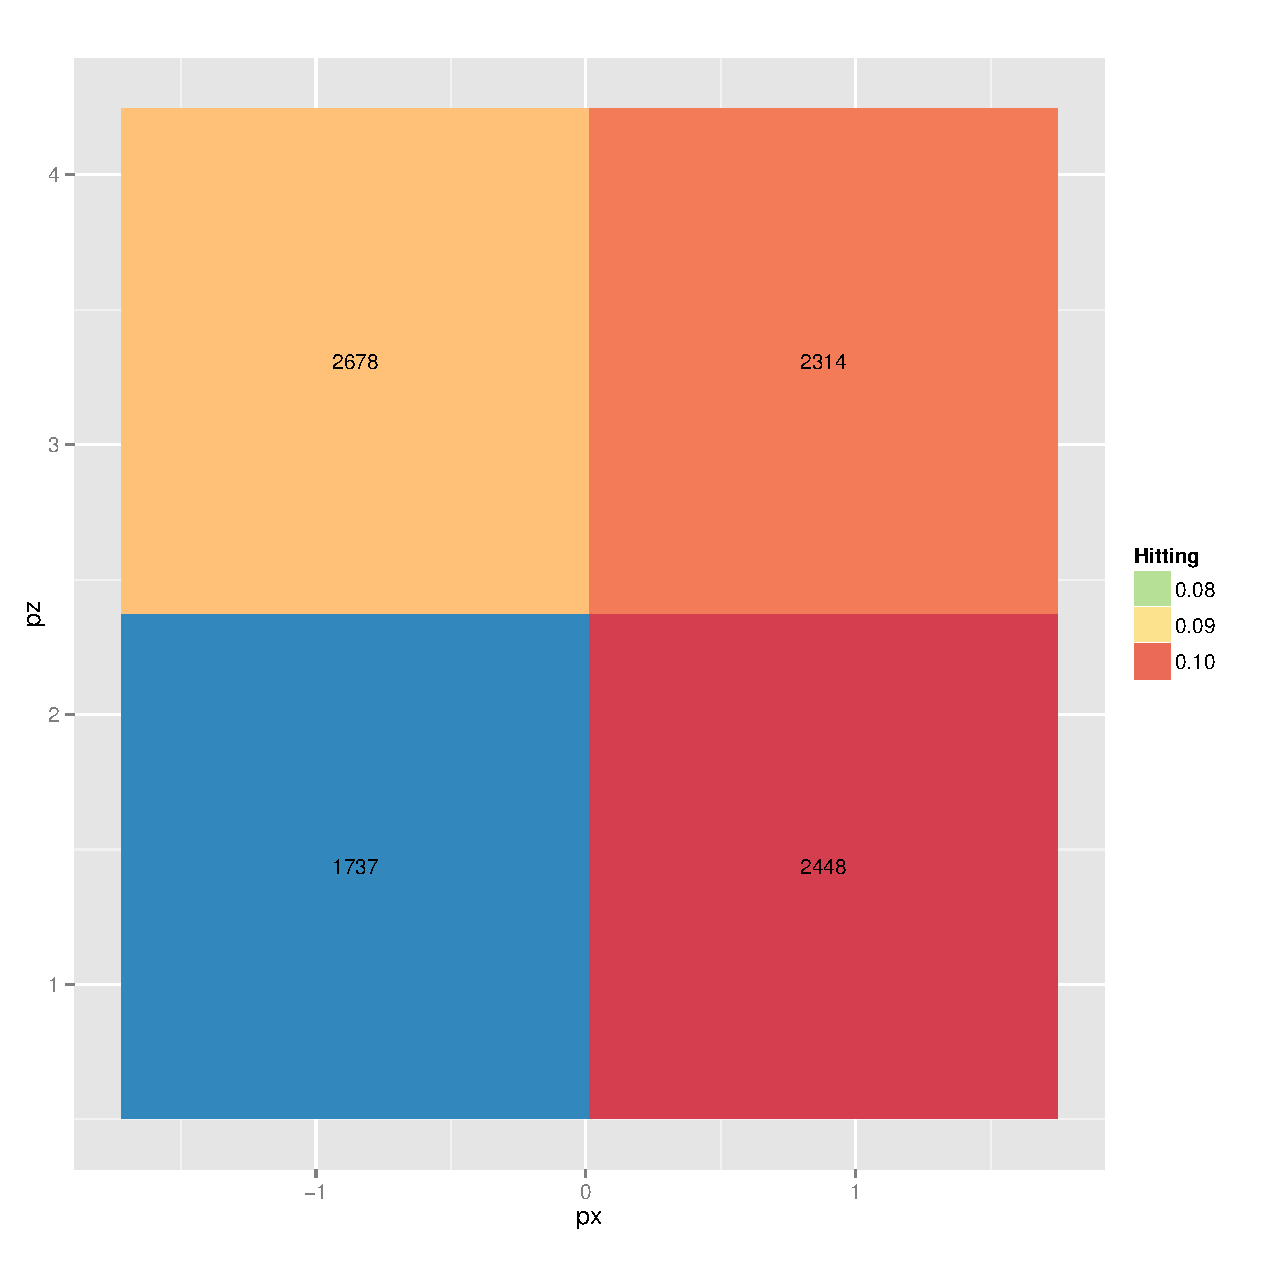
\includegraphics[scale=.05]{Images/Chapter2x2.jpg}
      	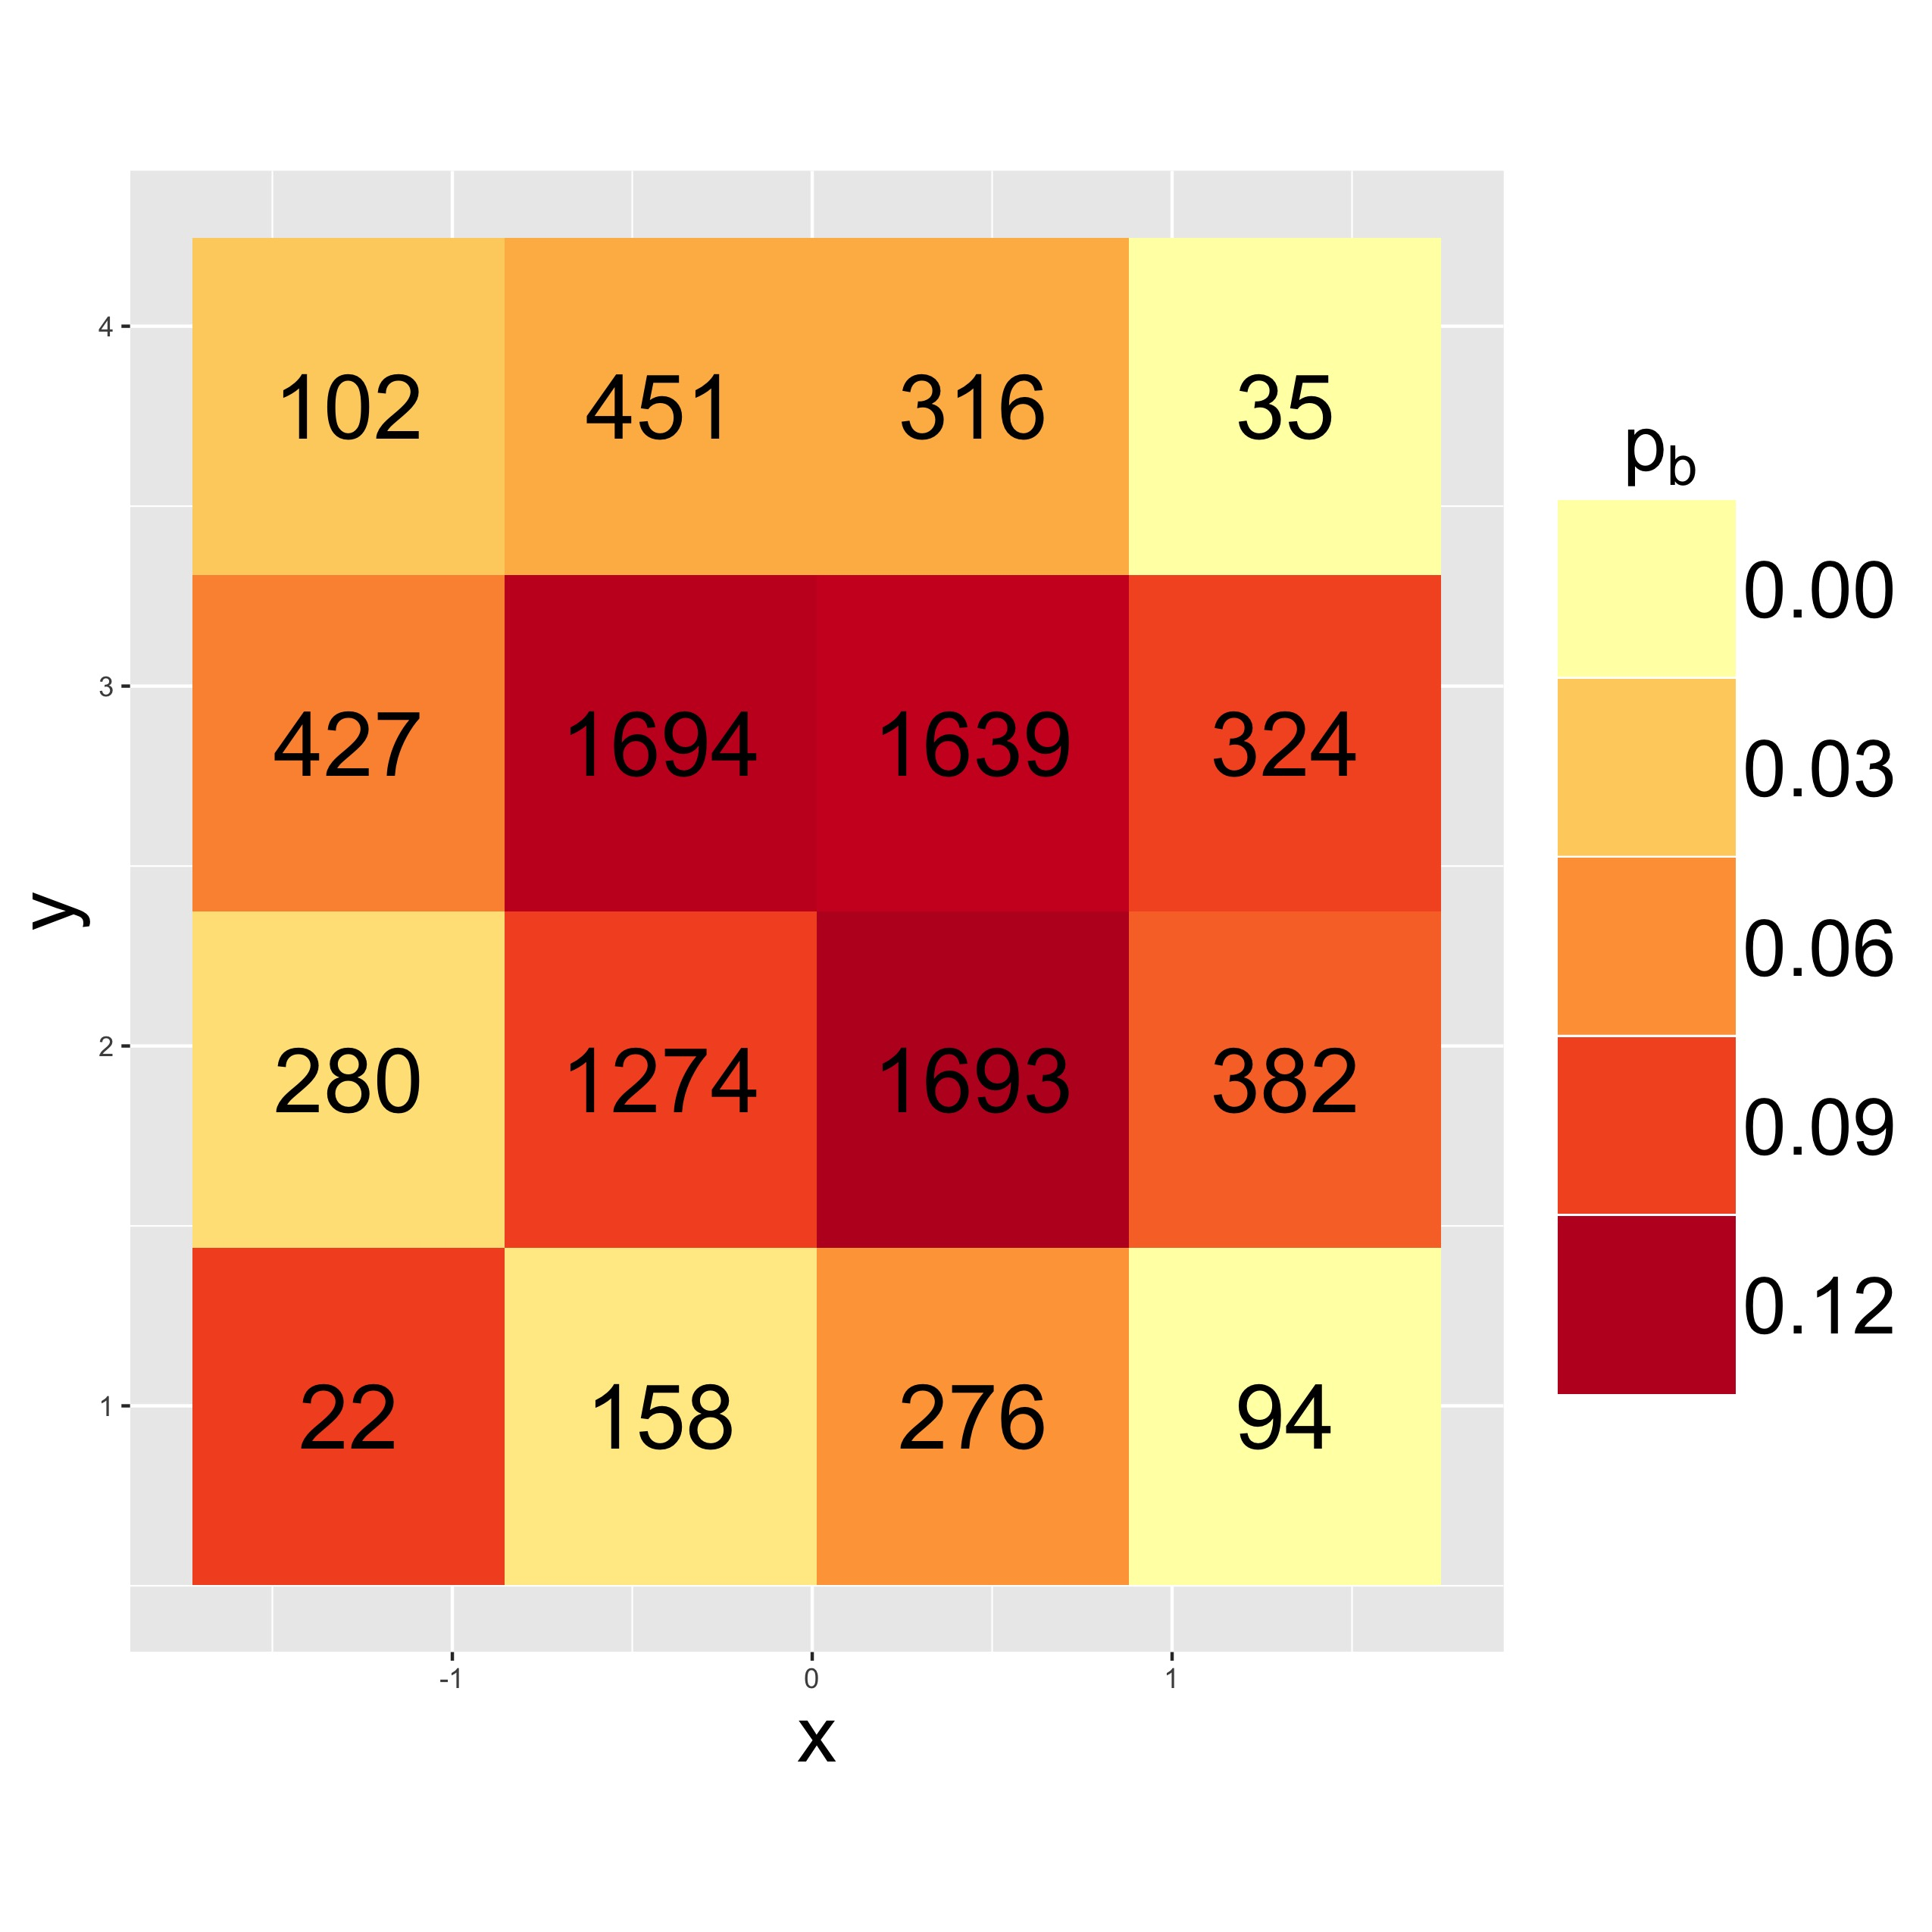
\includegraphics[scale=.05]{Images/Chapter4x4.jpg}
      	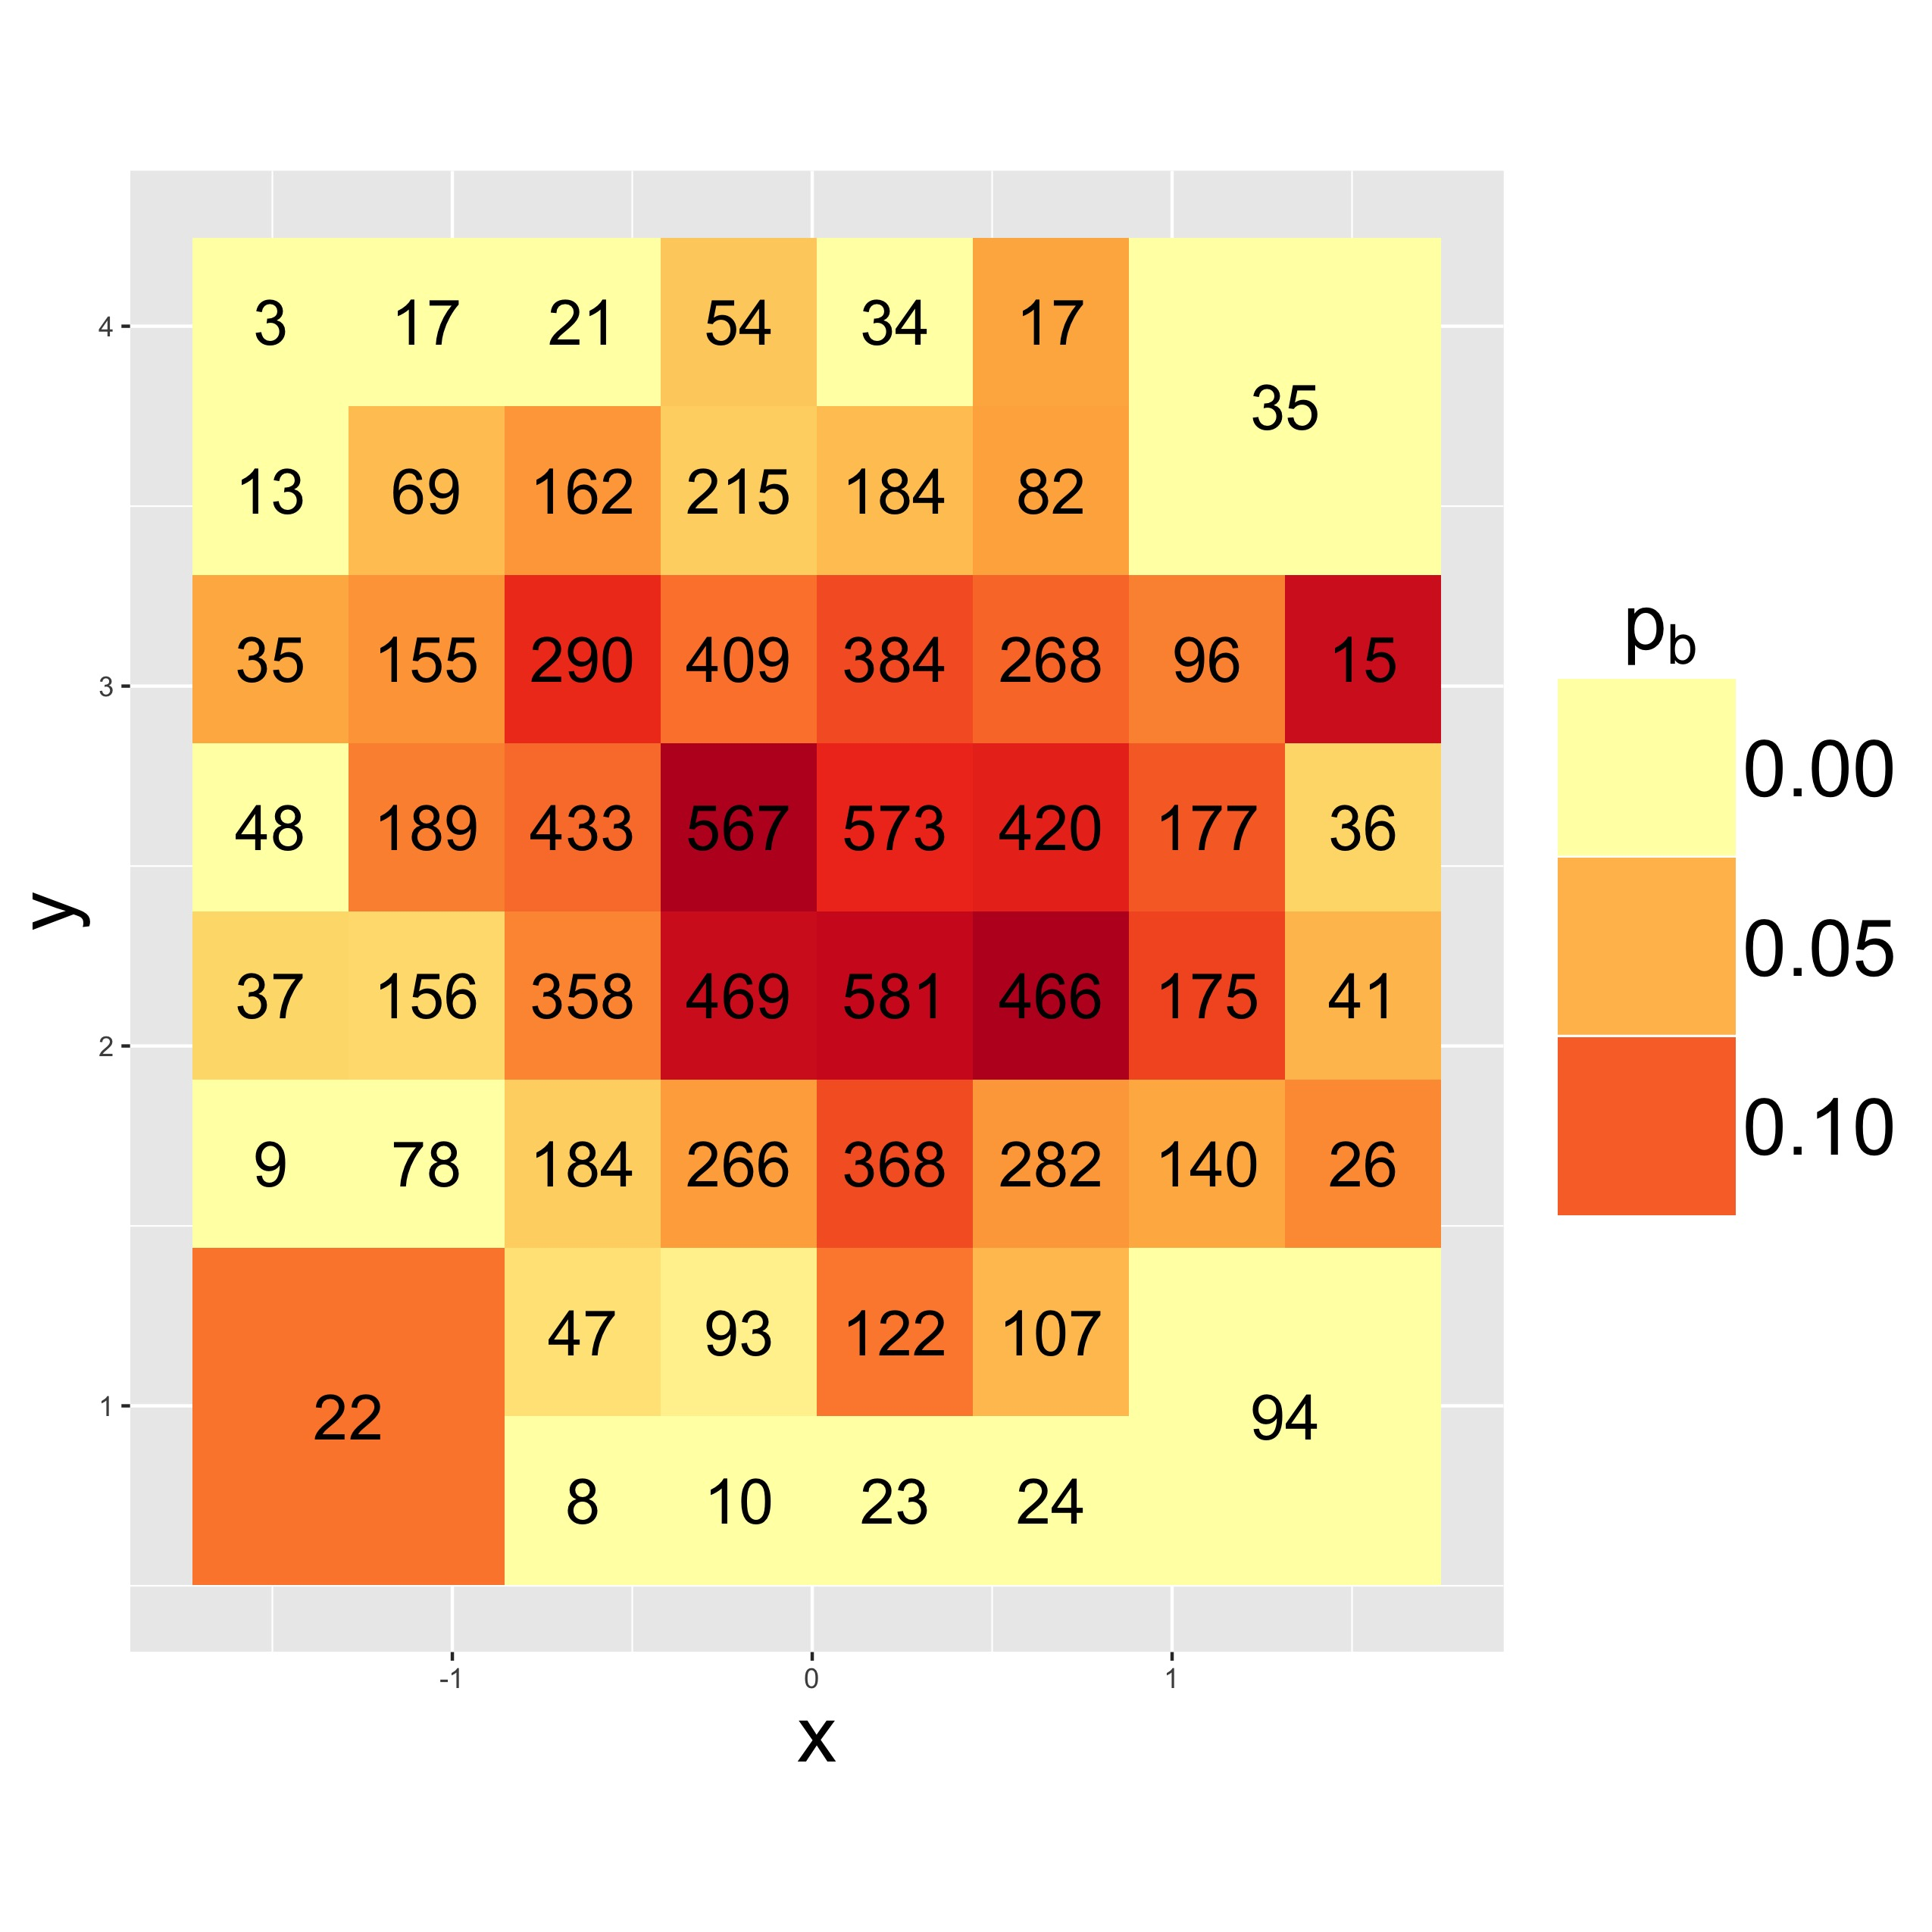
\includegraphics[scale=.05]{Images/Chapter8x8_100.jpg}
      	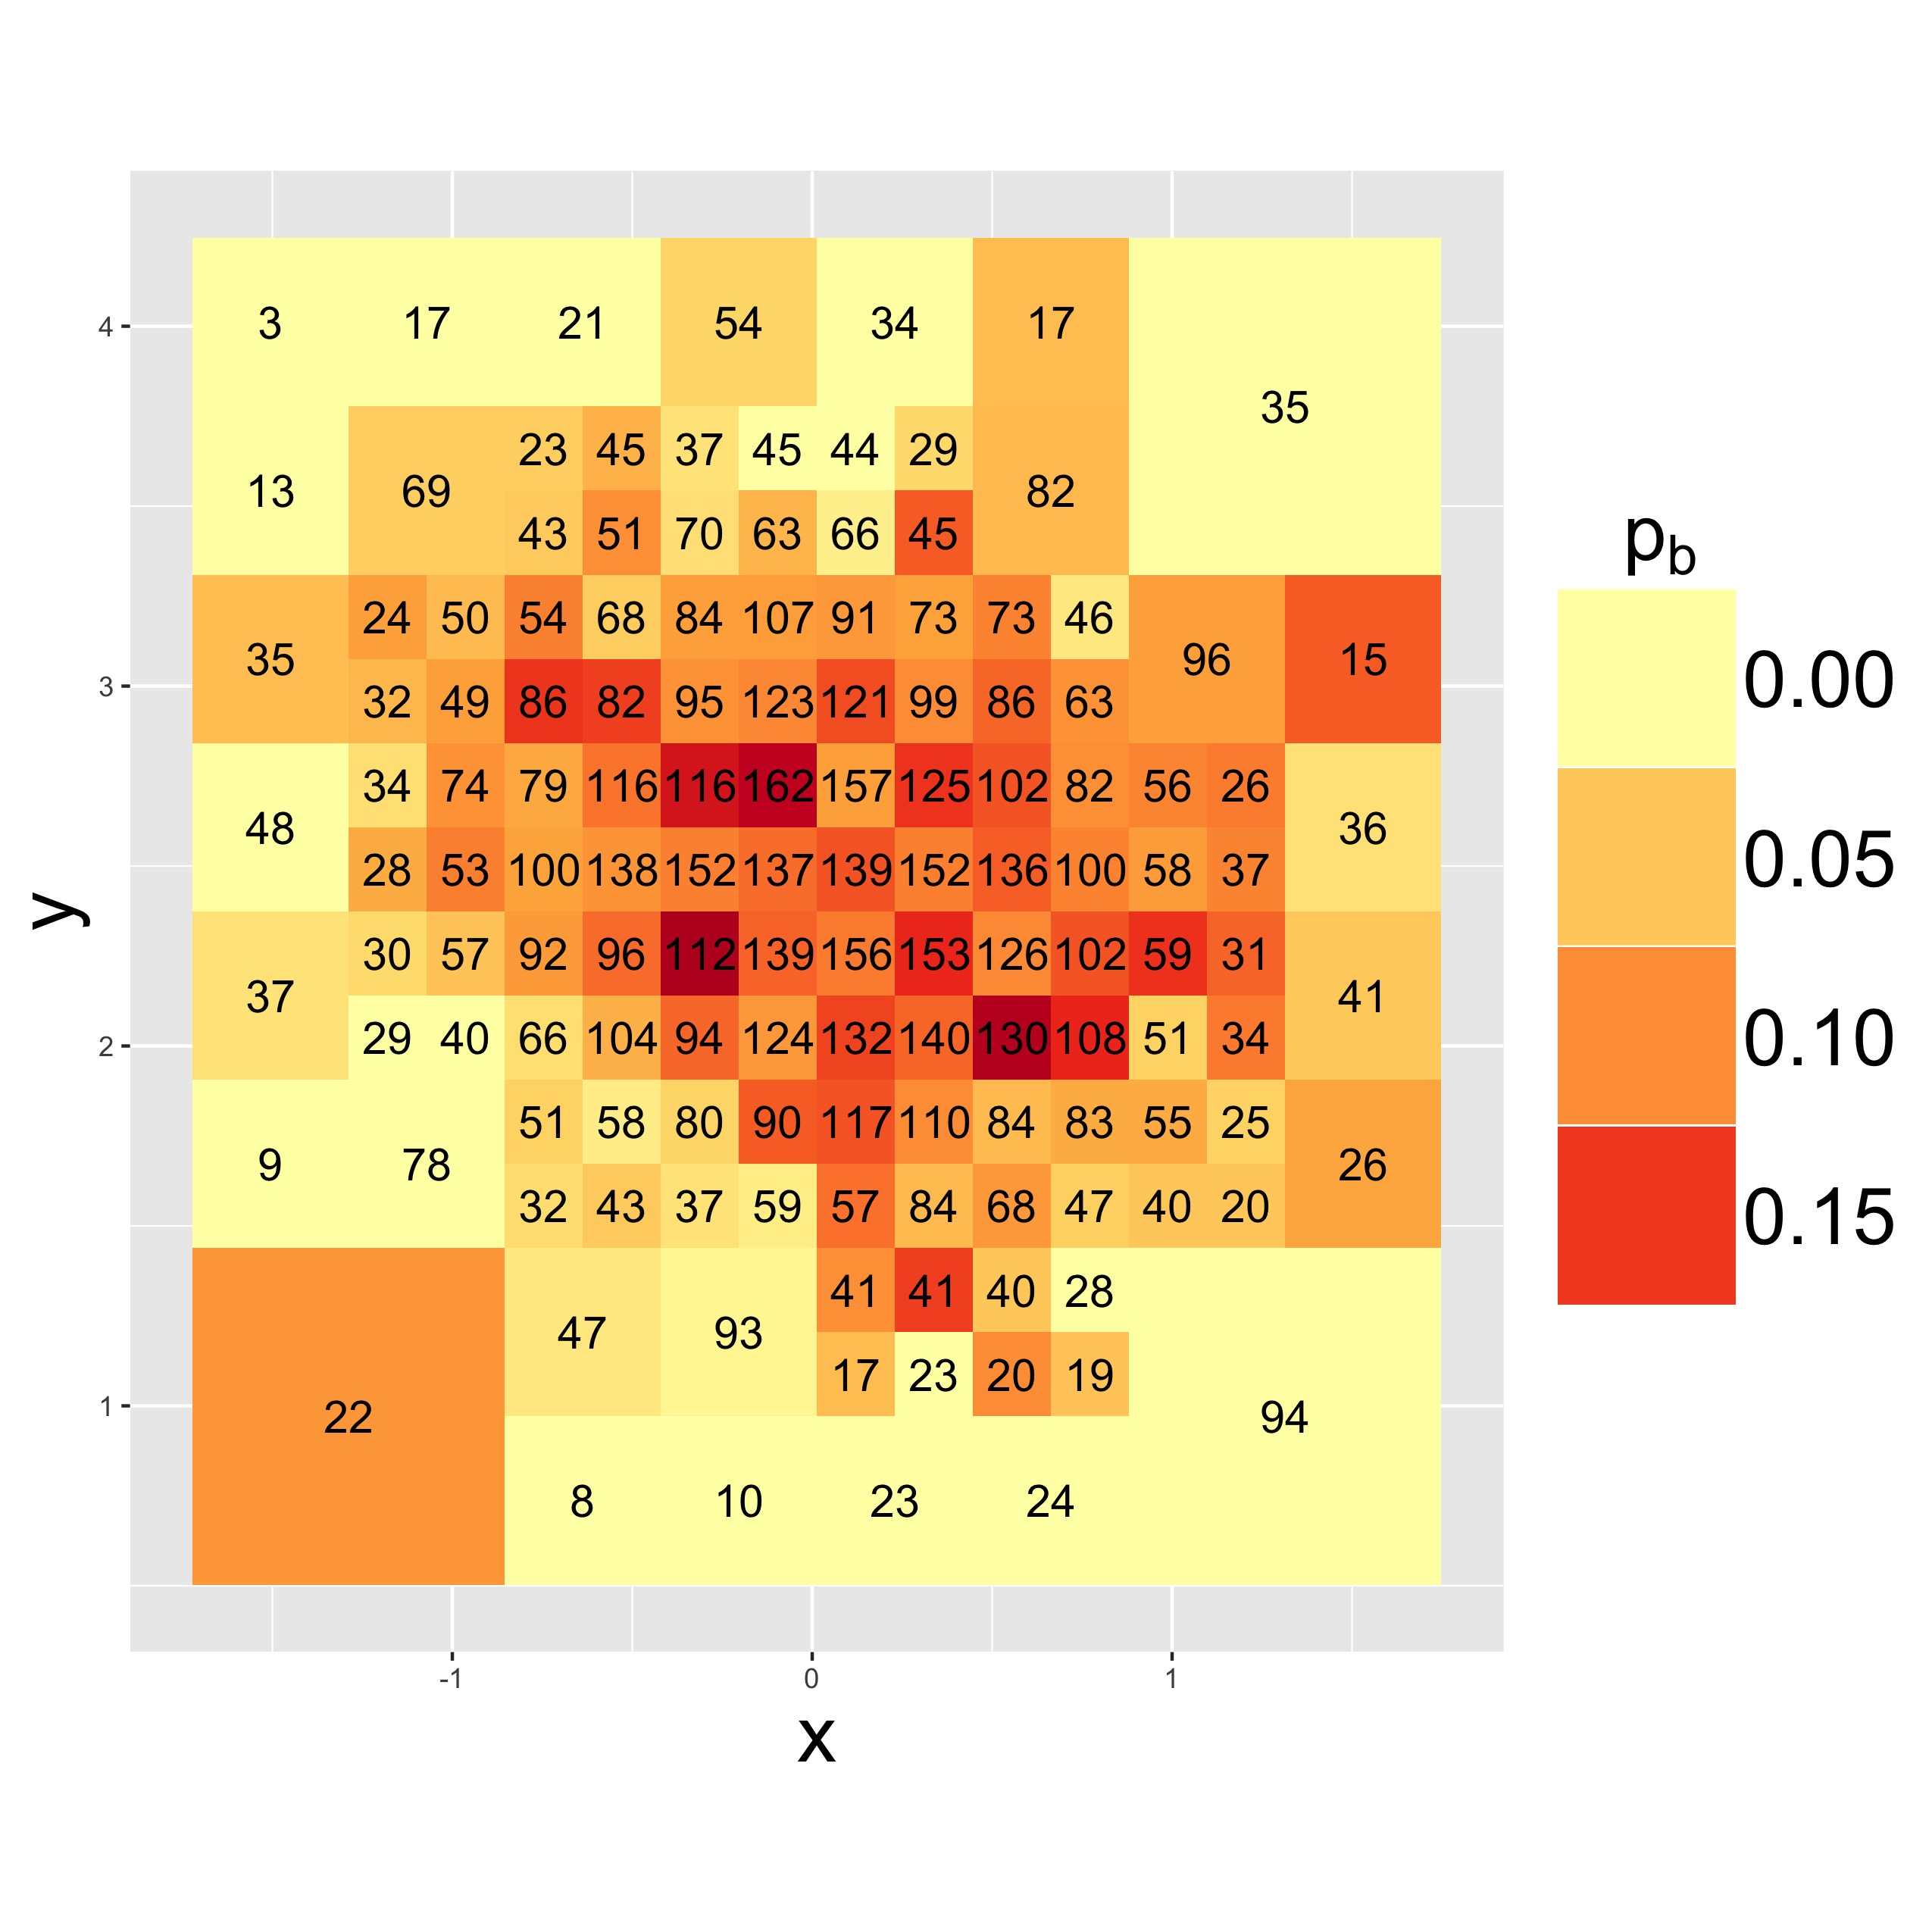
\includegraphics[scale=.05]{Images/Chapter16x16_100.jpg}
      	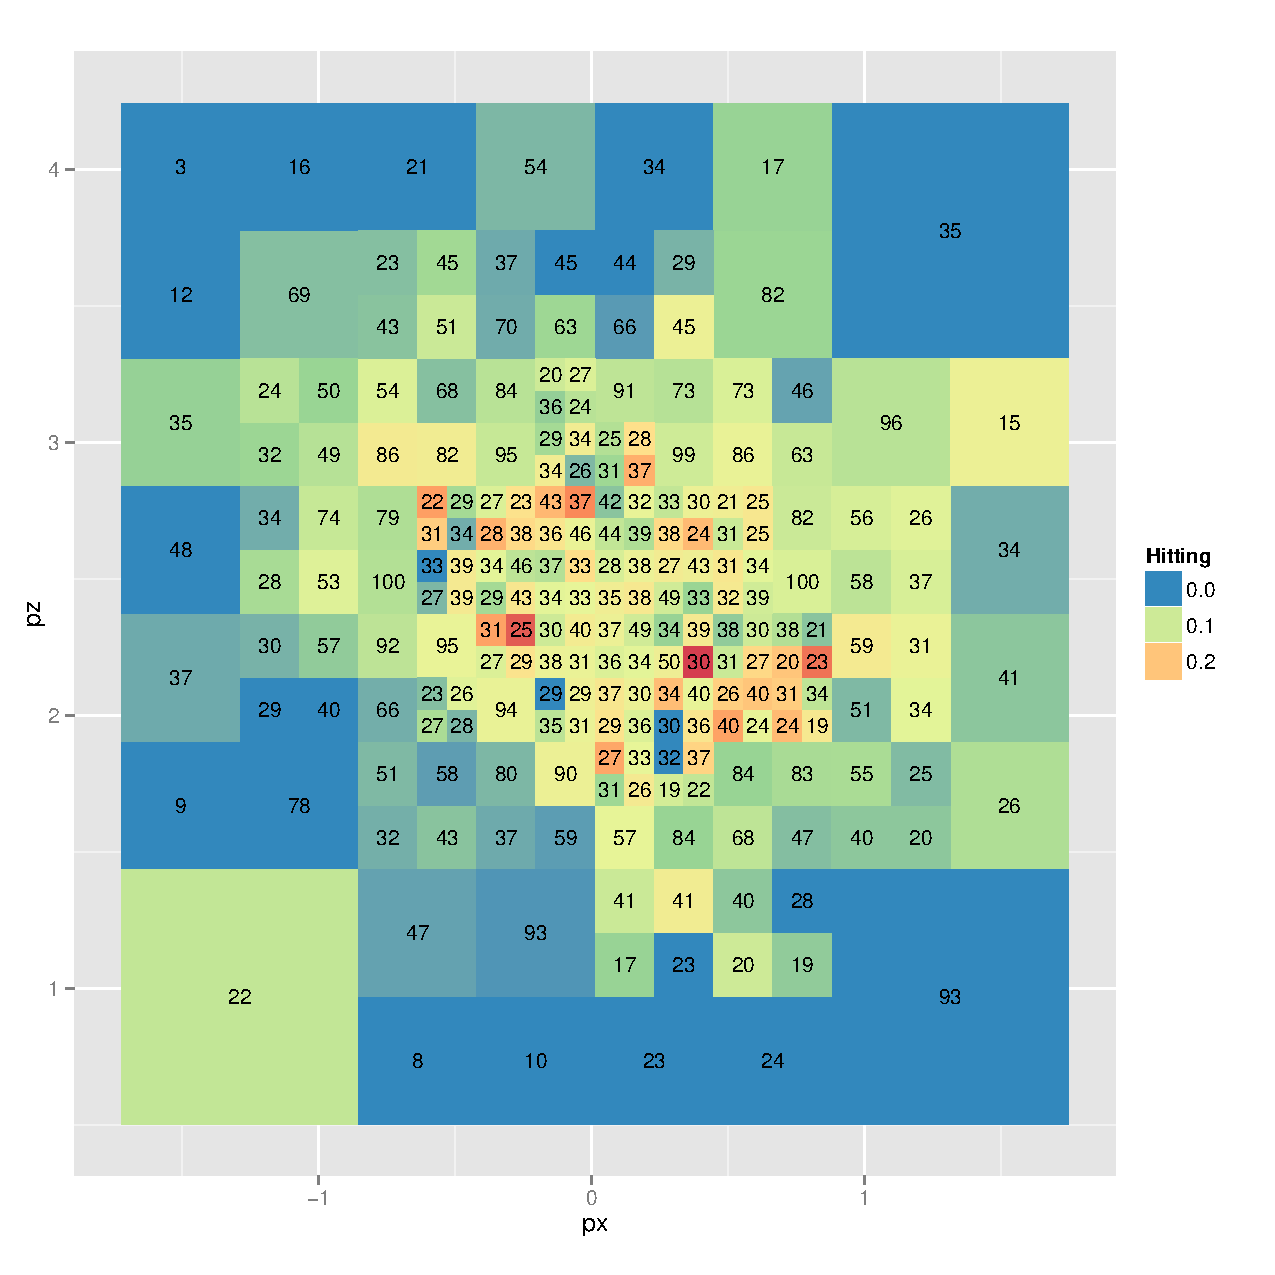
\includegraphics[scale=.05]{Images/Chapter32x32_100.jpg}
      	\caption{A variable-resolution heat map sequence. Starting from the top left and moving across, the algorithm subdivides all boxes with a sample size (printed on box) greater than 100. The maps convey Jhonny Peralta's empirical success probability by mapping $\hat{p}_{b}$ to a color.}
      	\lable{fig:altsr}
\end{figure} 	

Compare Figure \ref{fig:altsr} for stopping rule $n_{b} < 100$, to Figure \ref{fig:allvr} for stopping rule $n_{b} < 200$; the first three maps in each sequence match exactly. However, notice the resolution toward the center of the last heat map increased beyond what we saw before with $n_{b} < 200$ maps. For baseball data this resolution increase may lack justification, but the cutoff component of the algorithm offers the flexibility to make that assessment and choose accordingly. Also, notice Box 158 and Box 102 in the $4 \times 4$ heat map; both boxes have sample sizes {\it between} the two stopping rules. Because of this fact, we see diverging paths, where one stopping rule prevents further subdivision of those boxes, while the other compels it. Figure \ref{fig:vrcomp} shows the subsequent map for each stopping rule, with $n_{b} < 200$ on the left, and $n_{b} < 100$ on the right.
        \begin{figure}[H]
      	\centering      
      	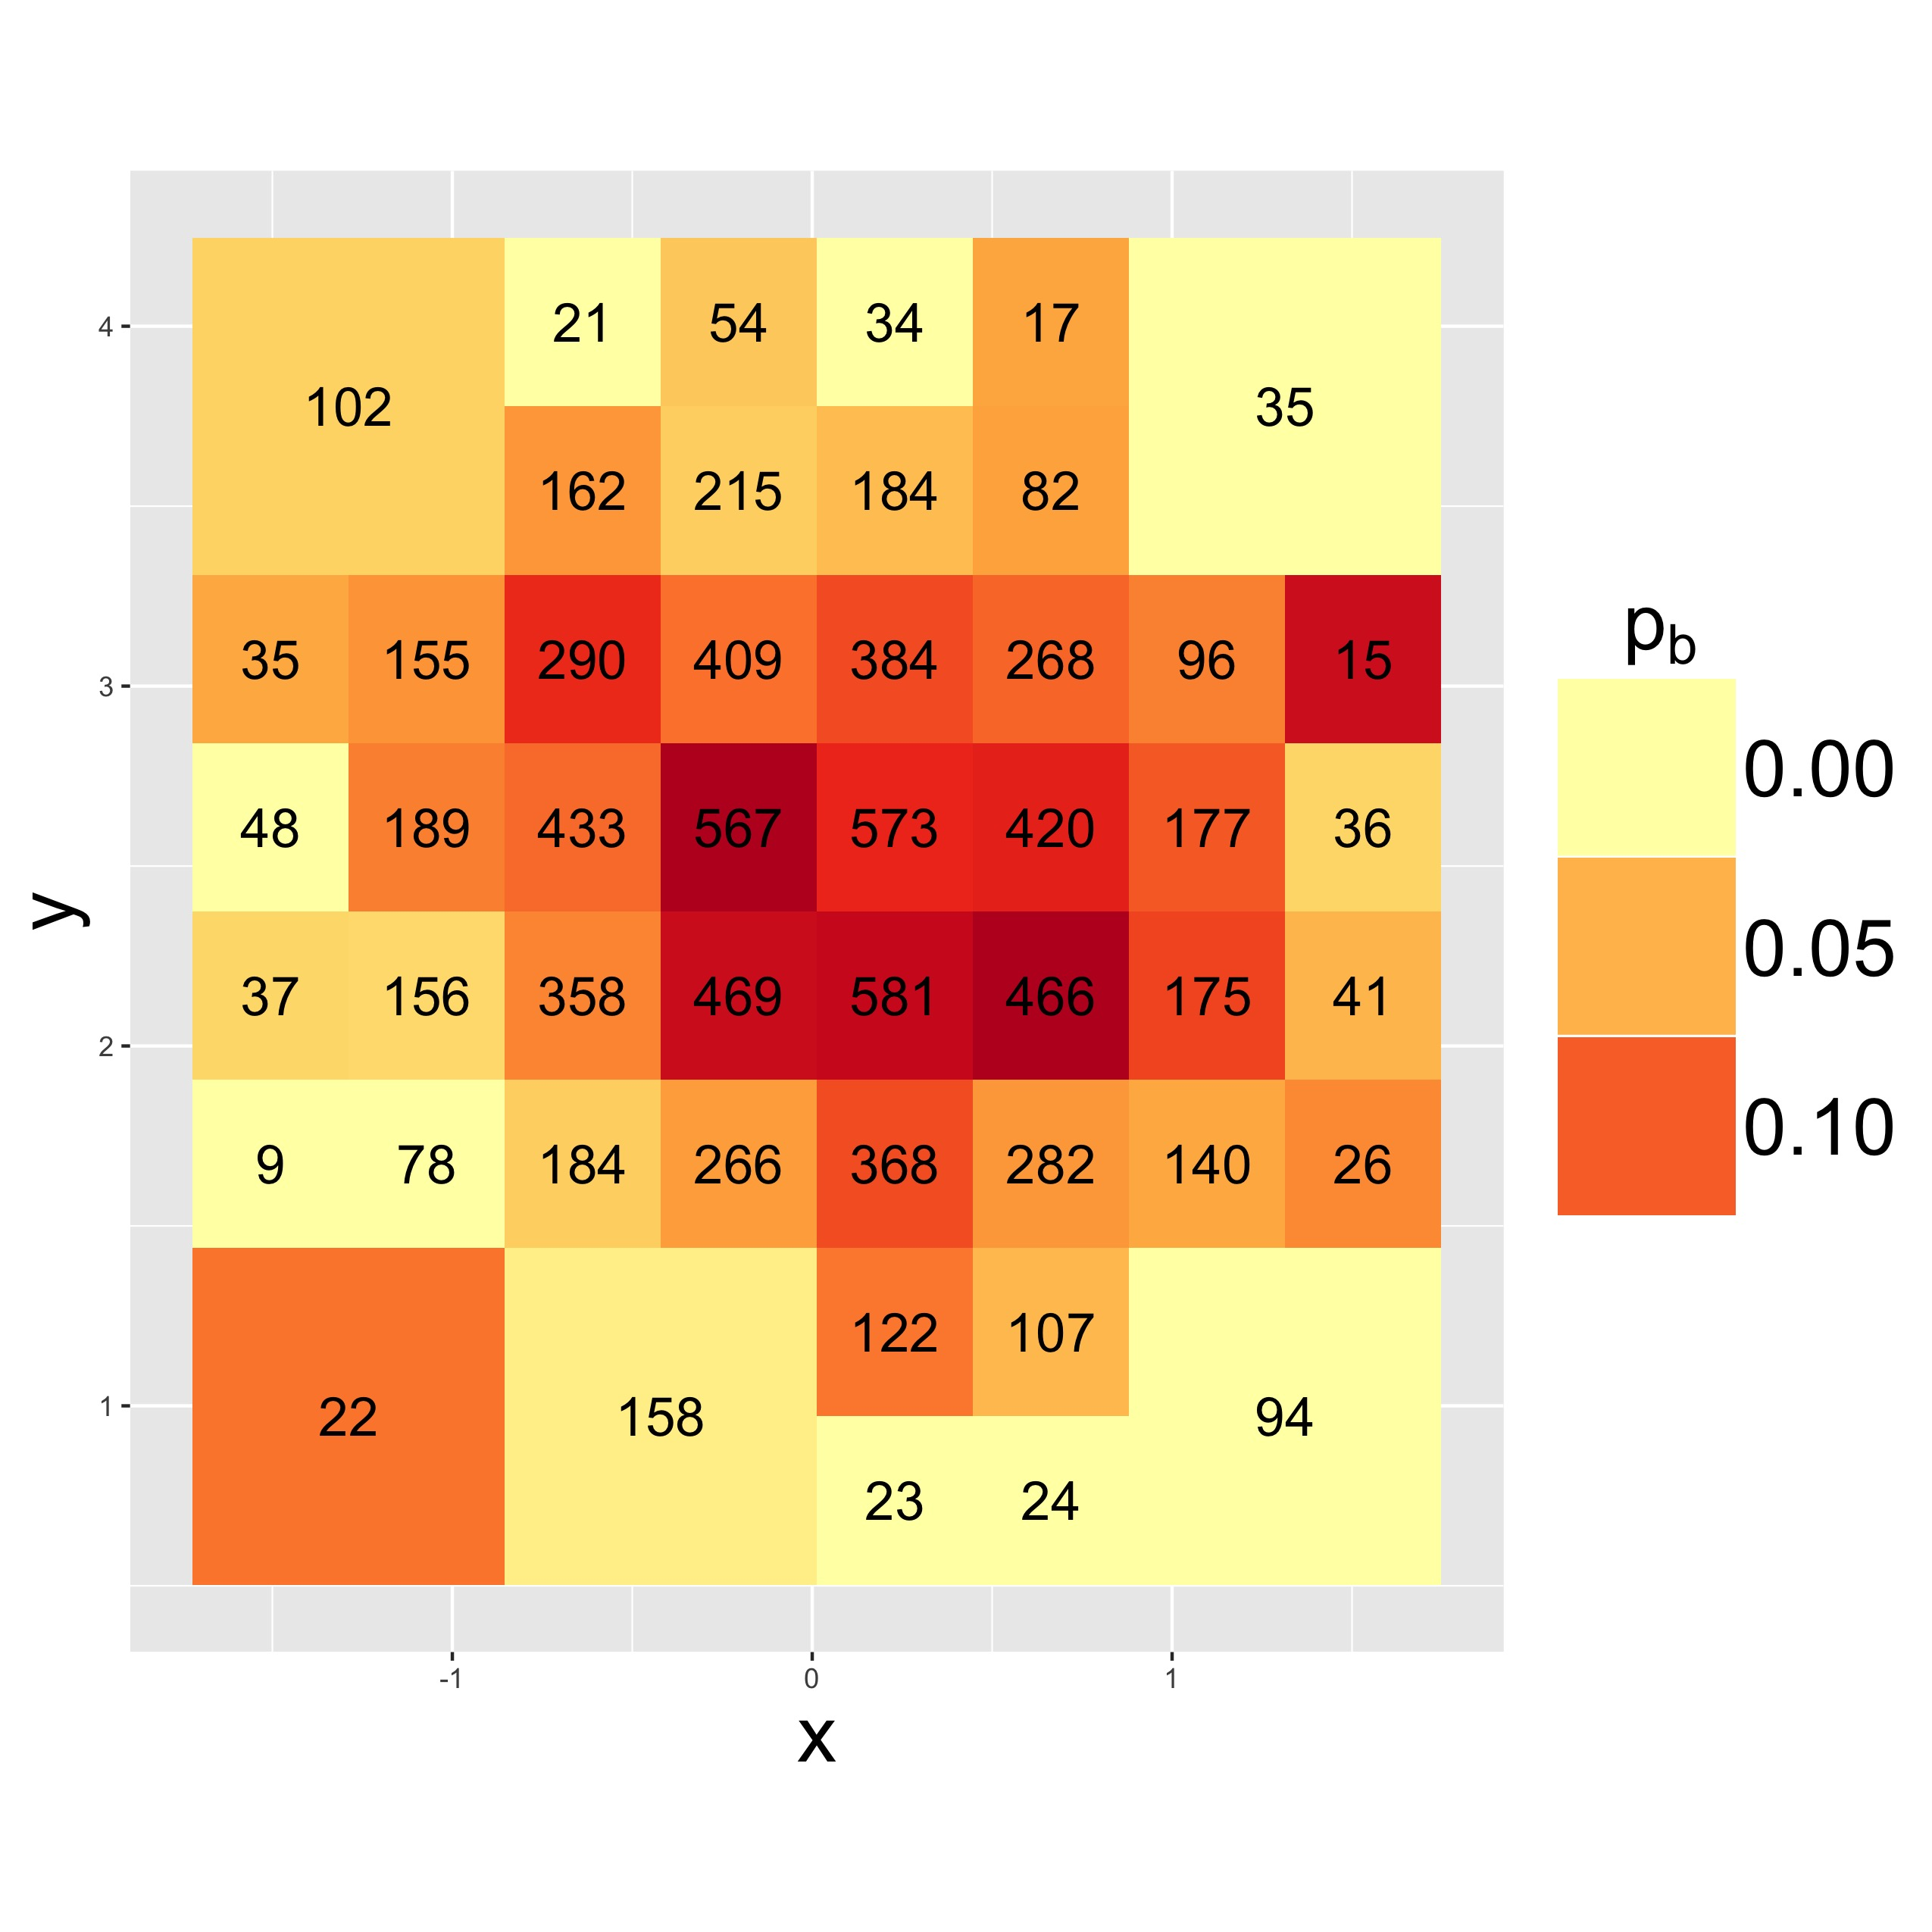
\includegraphics[scale=.05]{Images/Chapter8x8_200.jpg}
      	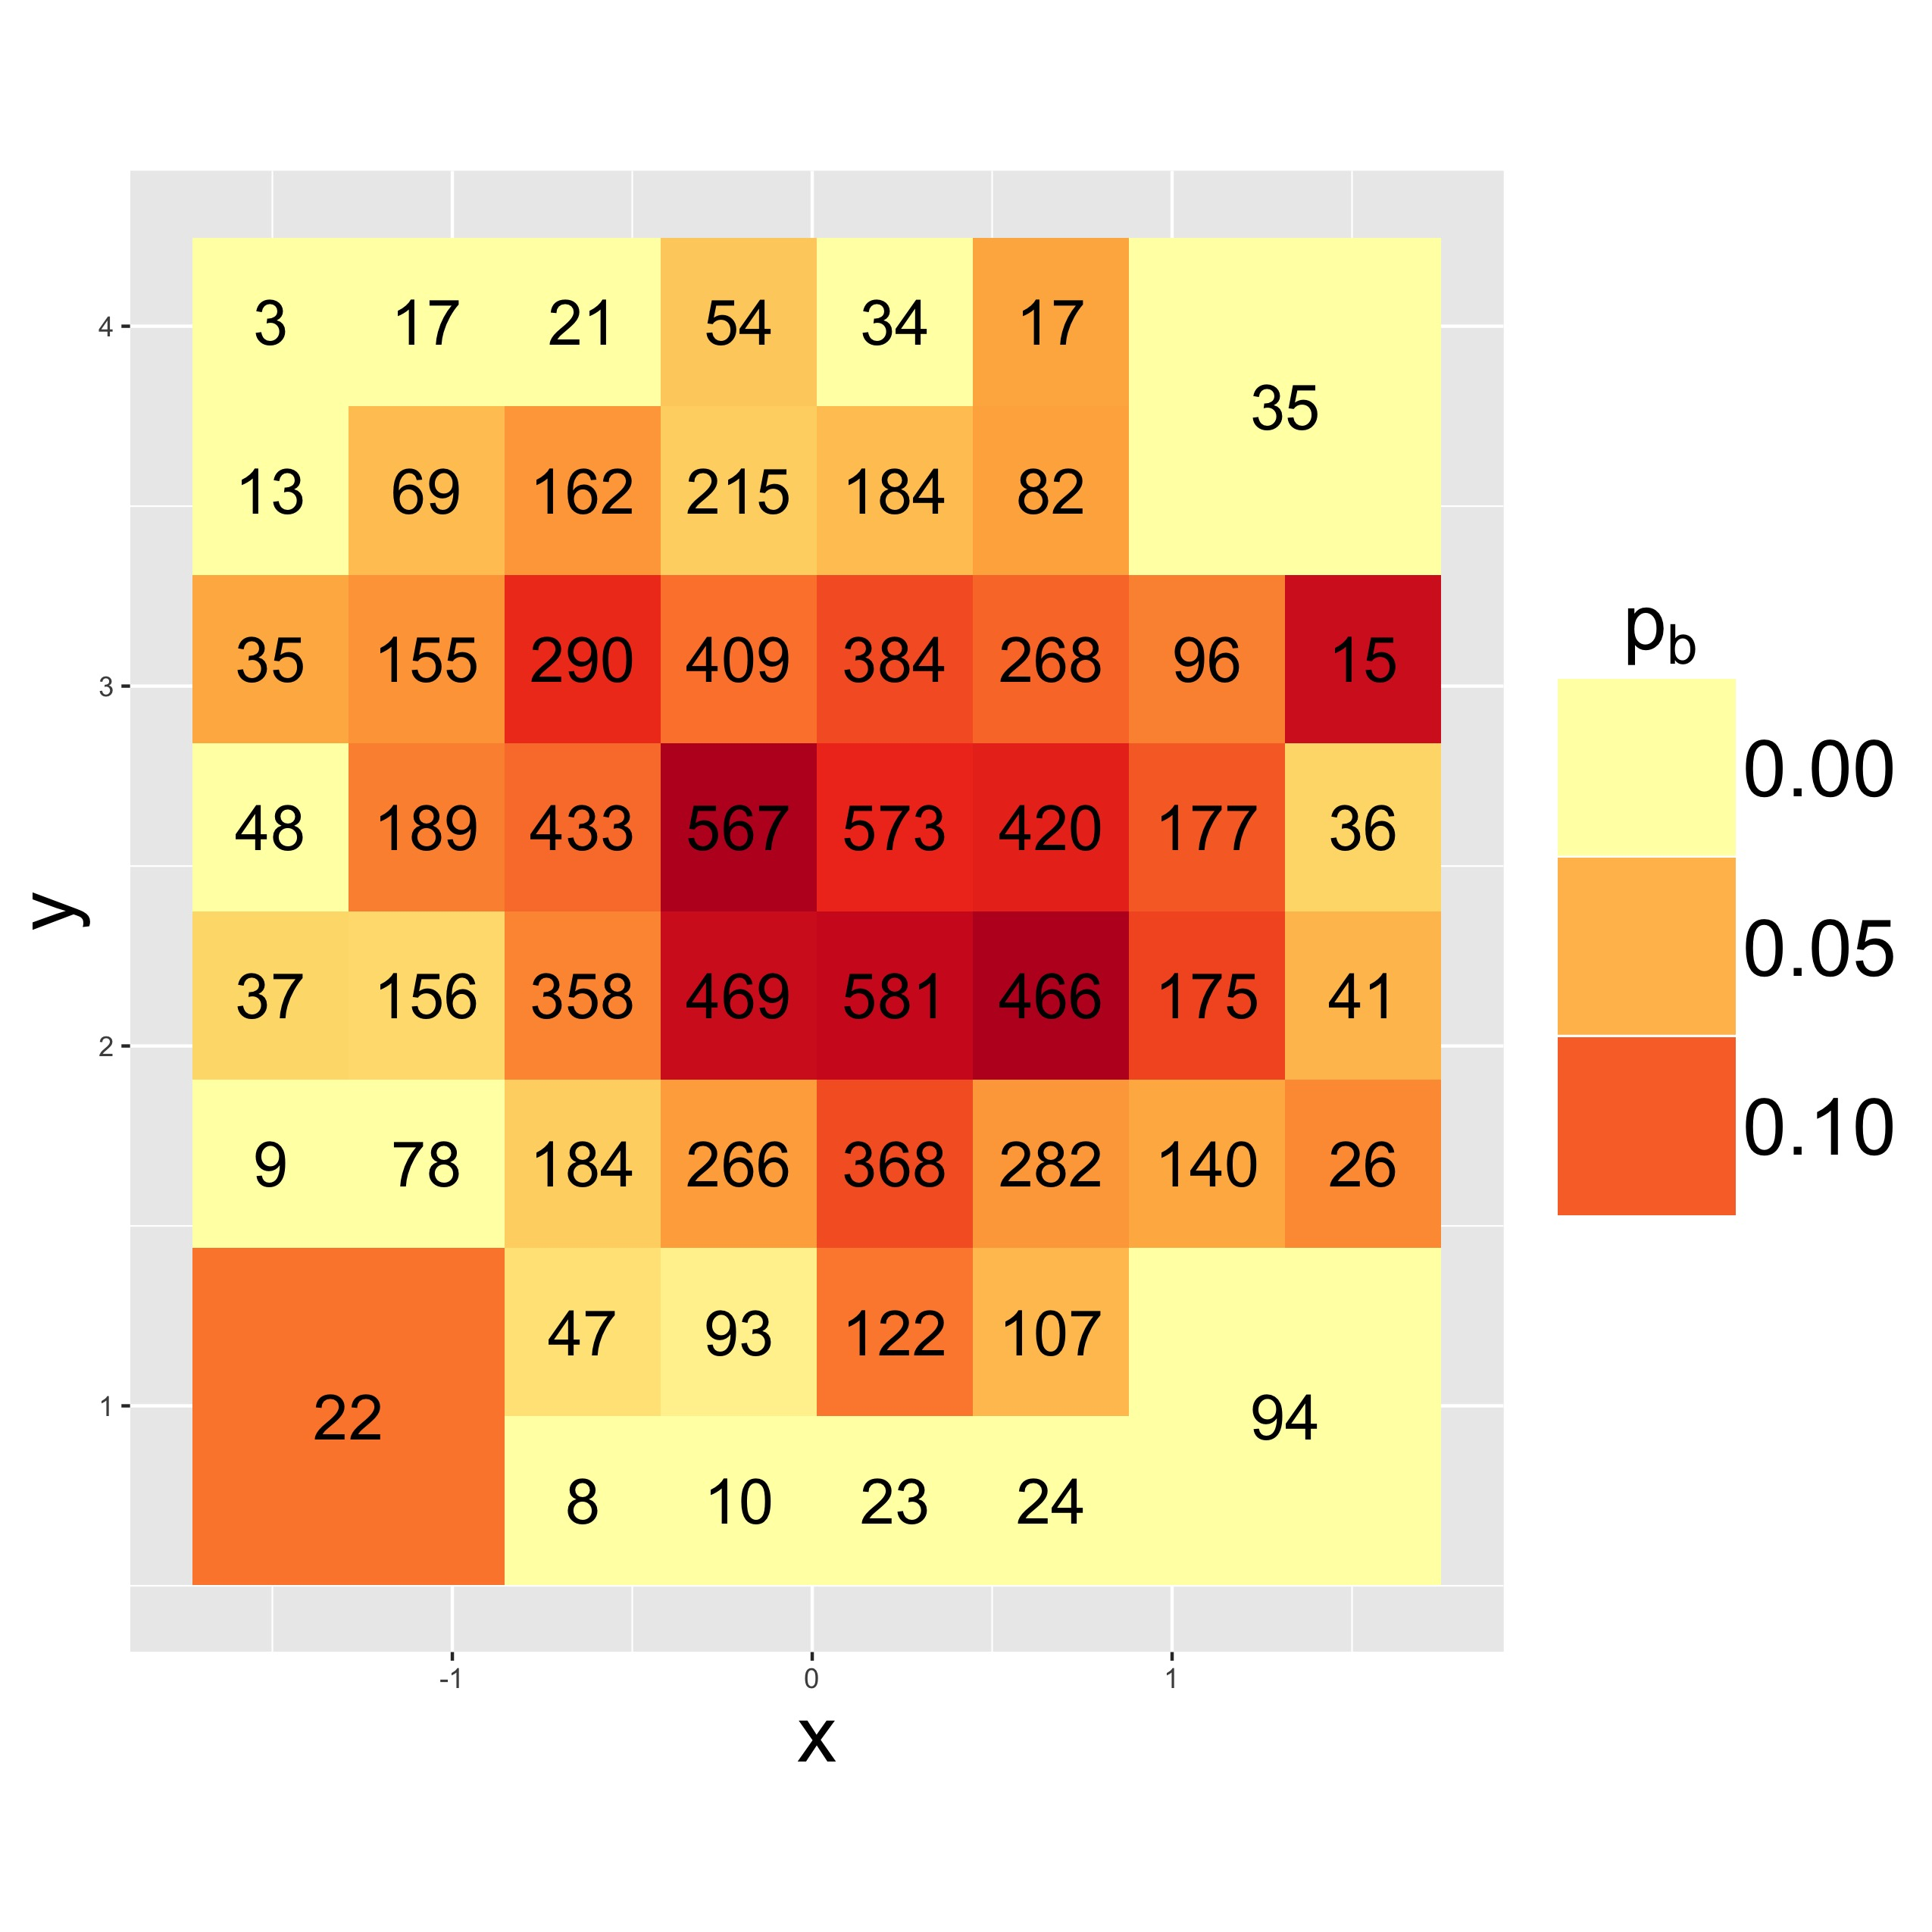
\includegraphics[scale=.05]{Images/Chapter8x8_100.jpg}
      	\caption{Variable-resolution heat maps diverge when box totals fall between sample size stopping rules. Boxes 158 and 102 remain for stopping rule $n_{b} < 200$ (left), but further subdivide for stopping rule $n_{b} < 100$ (right).}
      	\label{fig:vrcomp}
\end{figure} 
The ``$n_{b} < 100$'' map now offers more spatial specificity at the former locations of Box 102 and Box 158. The heat maps also now differ in the number of boxes of each size, and the total number of boxes.  The differences increase at the next iteration, where stopping rule $n_{b} < 100$ produces 28 box subdivisions (Figure \ref{fig:altsr}); and $n_{b} < 200$ produces 16 box subdivisions (Figure \ref{fig:allvr}). Figure \ref{label:vrcomp2} shows two corresponding iterations for these two stopping rules with $n_{b} < 100$ in the top row, and $n_{b} < 200$ in the bottom row.
        \begin{figure}[H]
      	\centering      
      	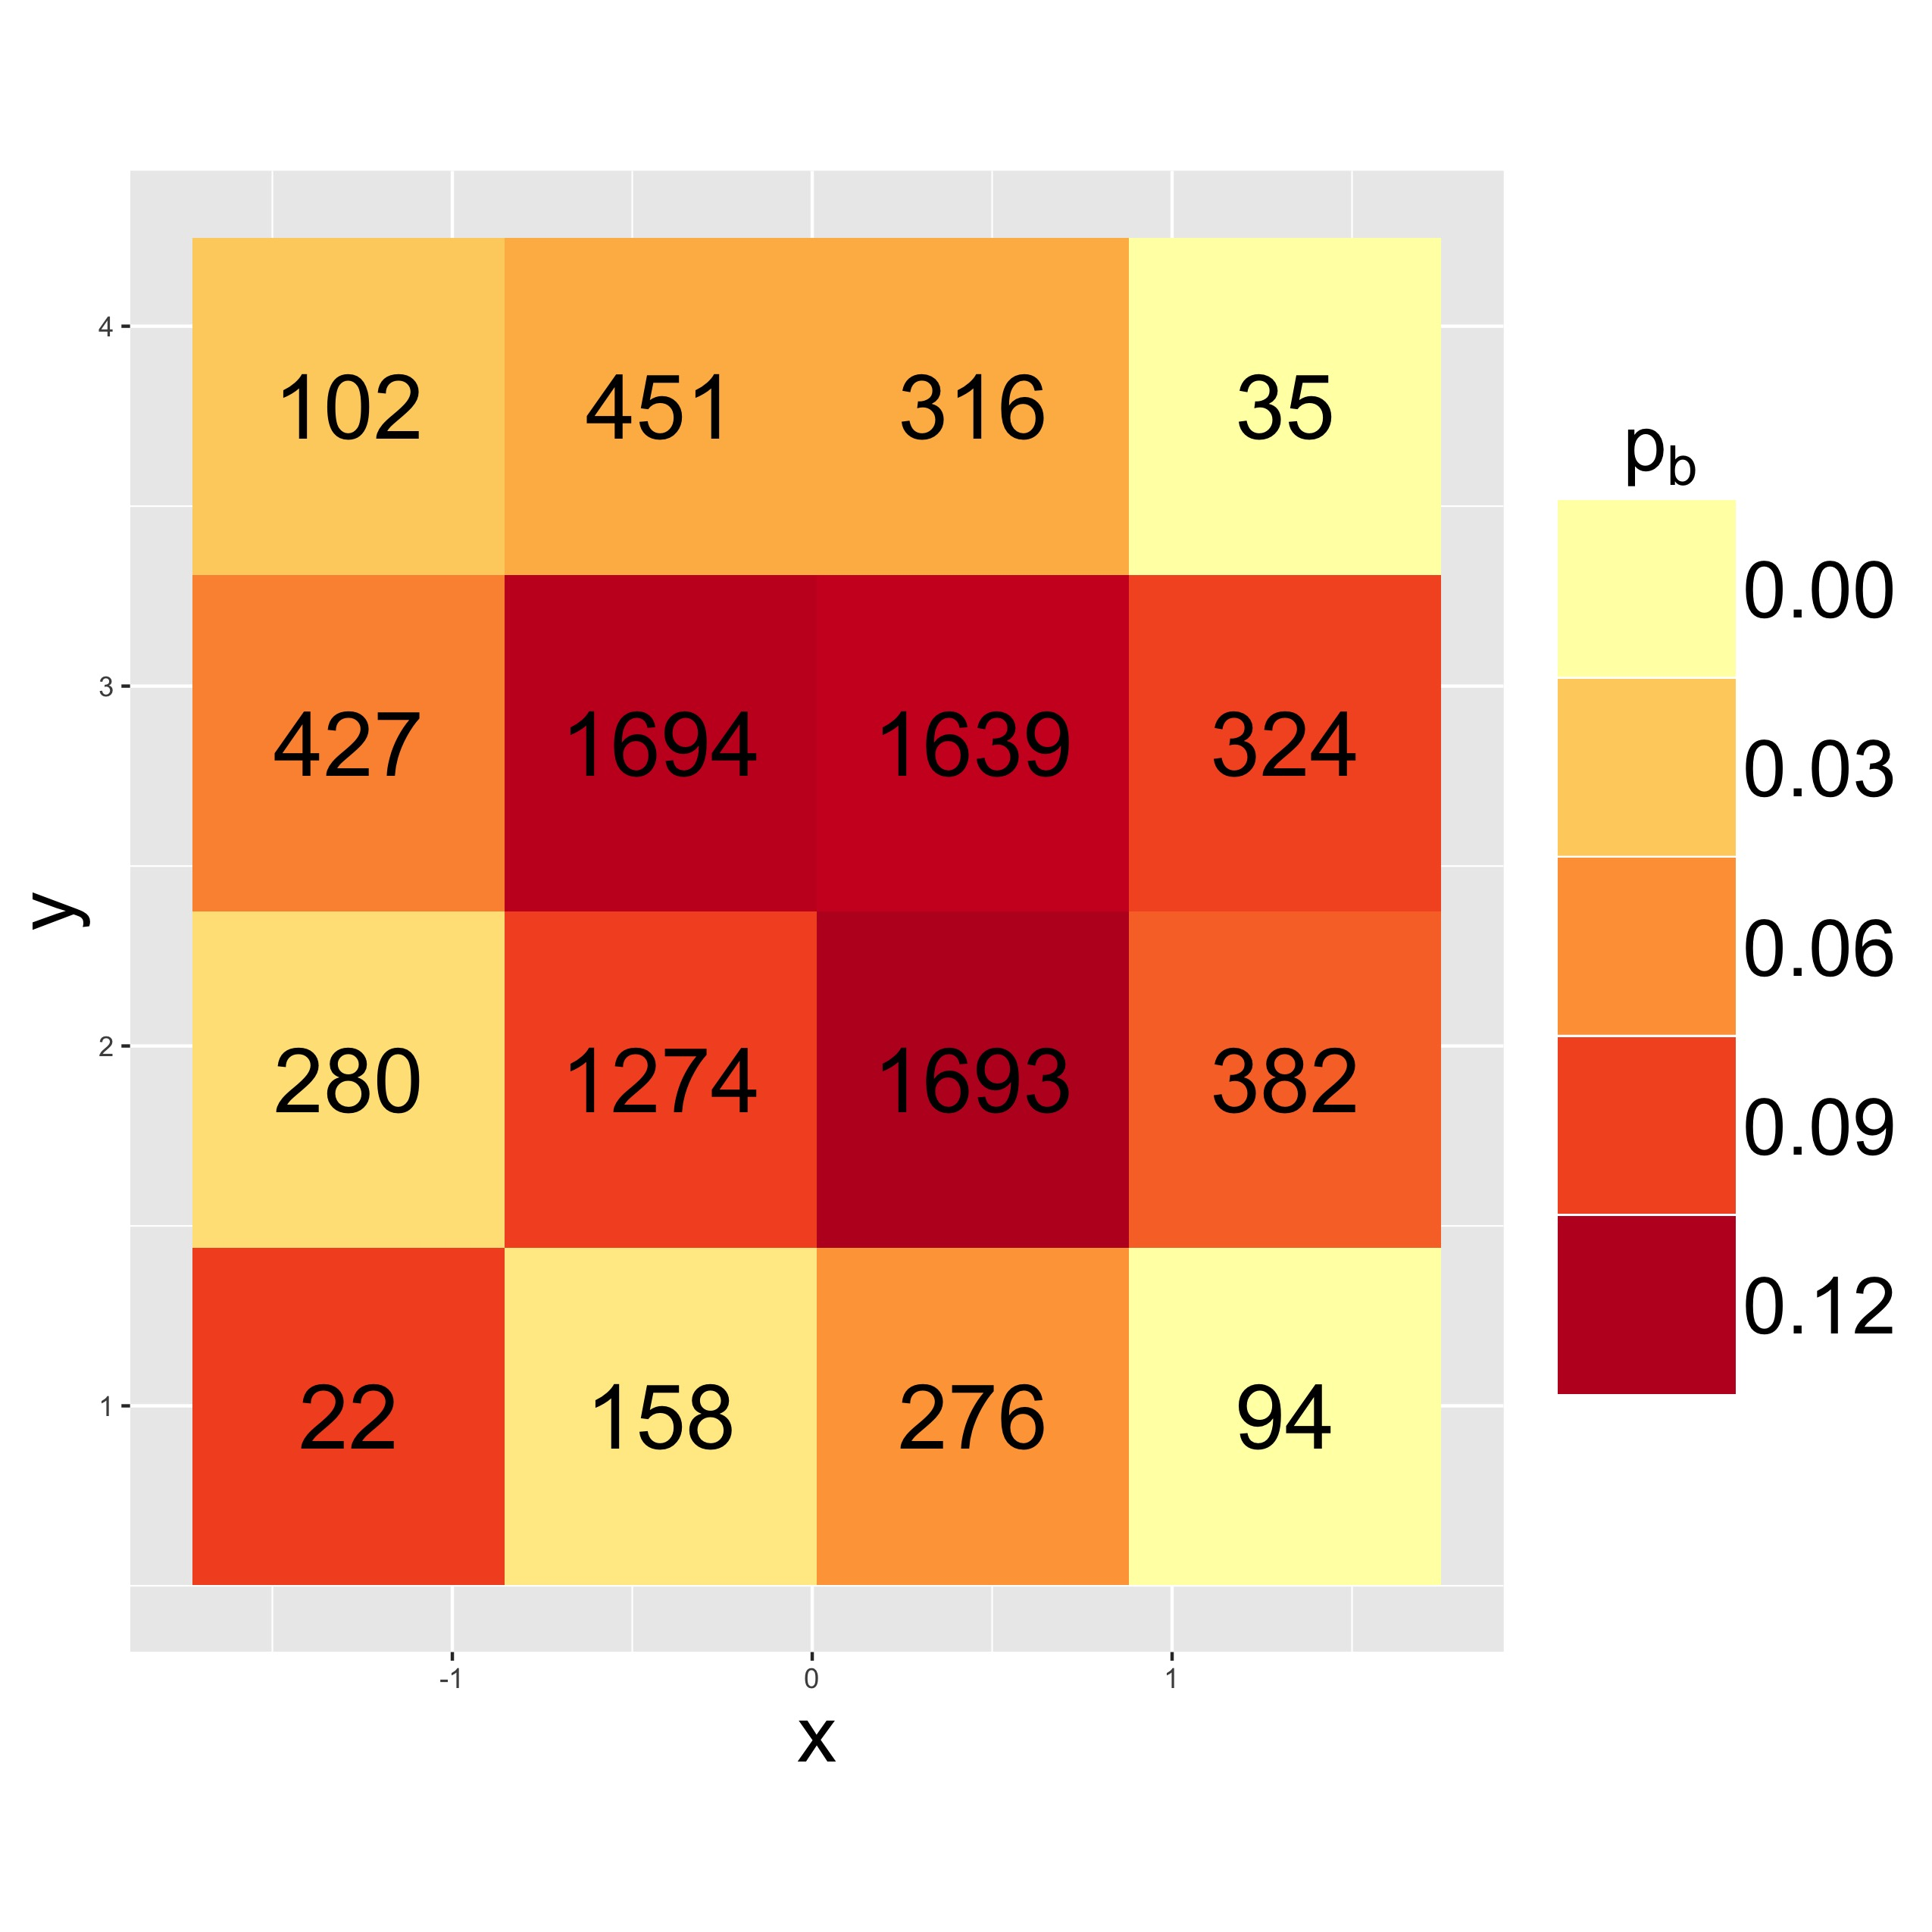
\includegraphics[scale=.05]{Images/Chapter4x4.jpg}
      	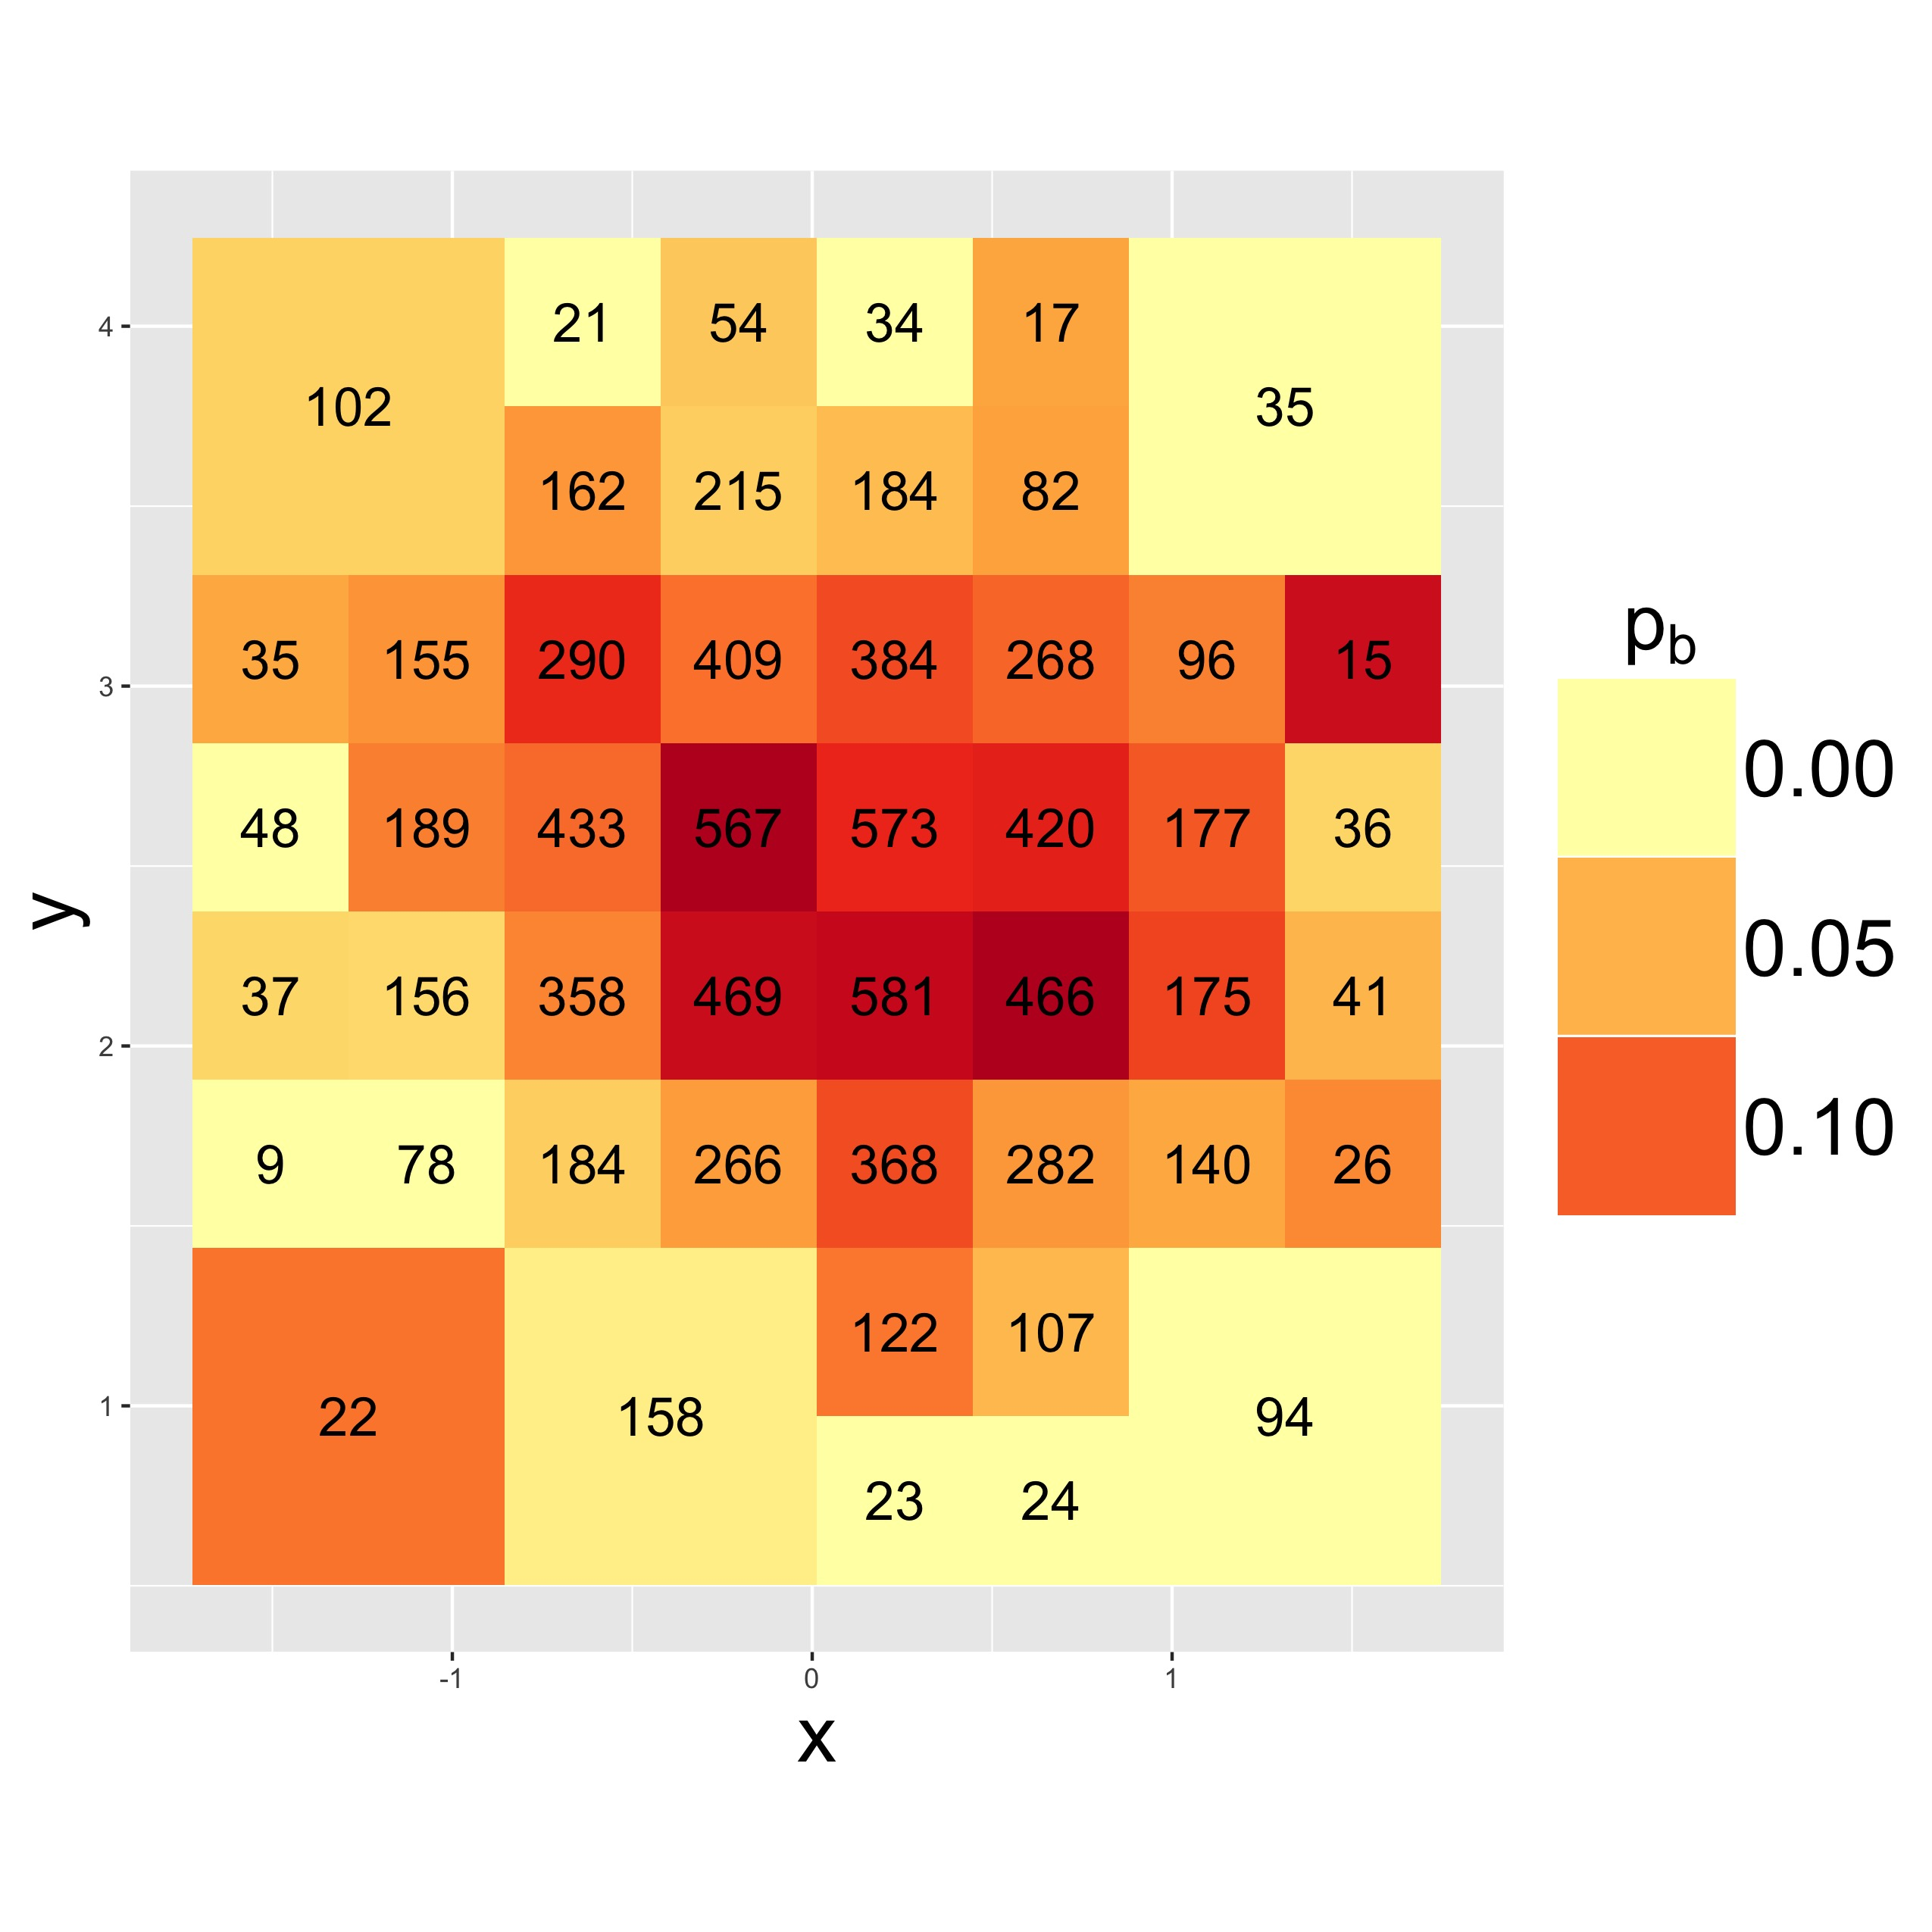
\includegraphics[scale=.05]{Images/Chapter8x8_200.jpg}
      	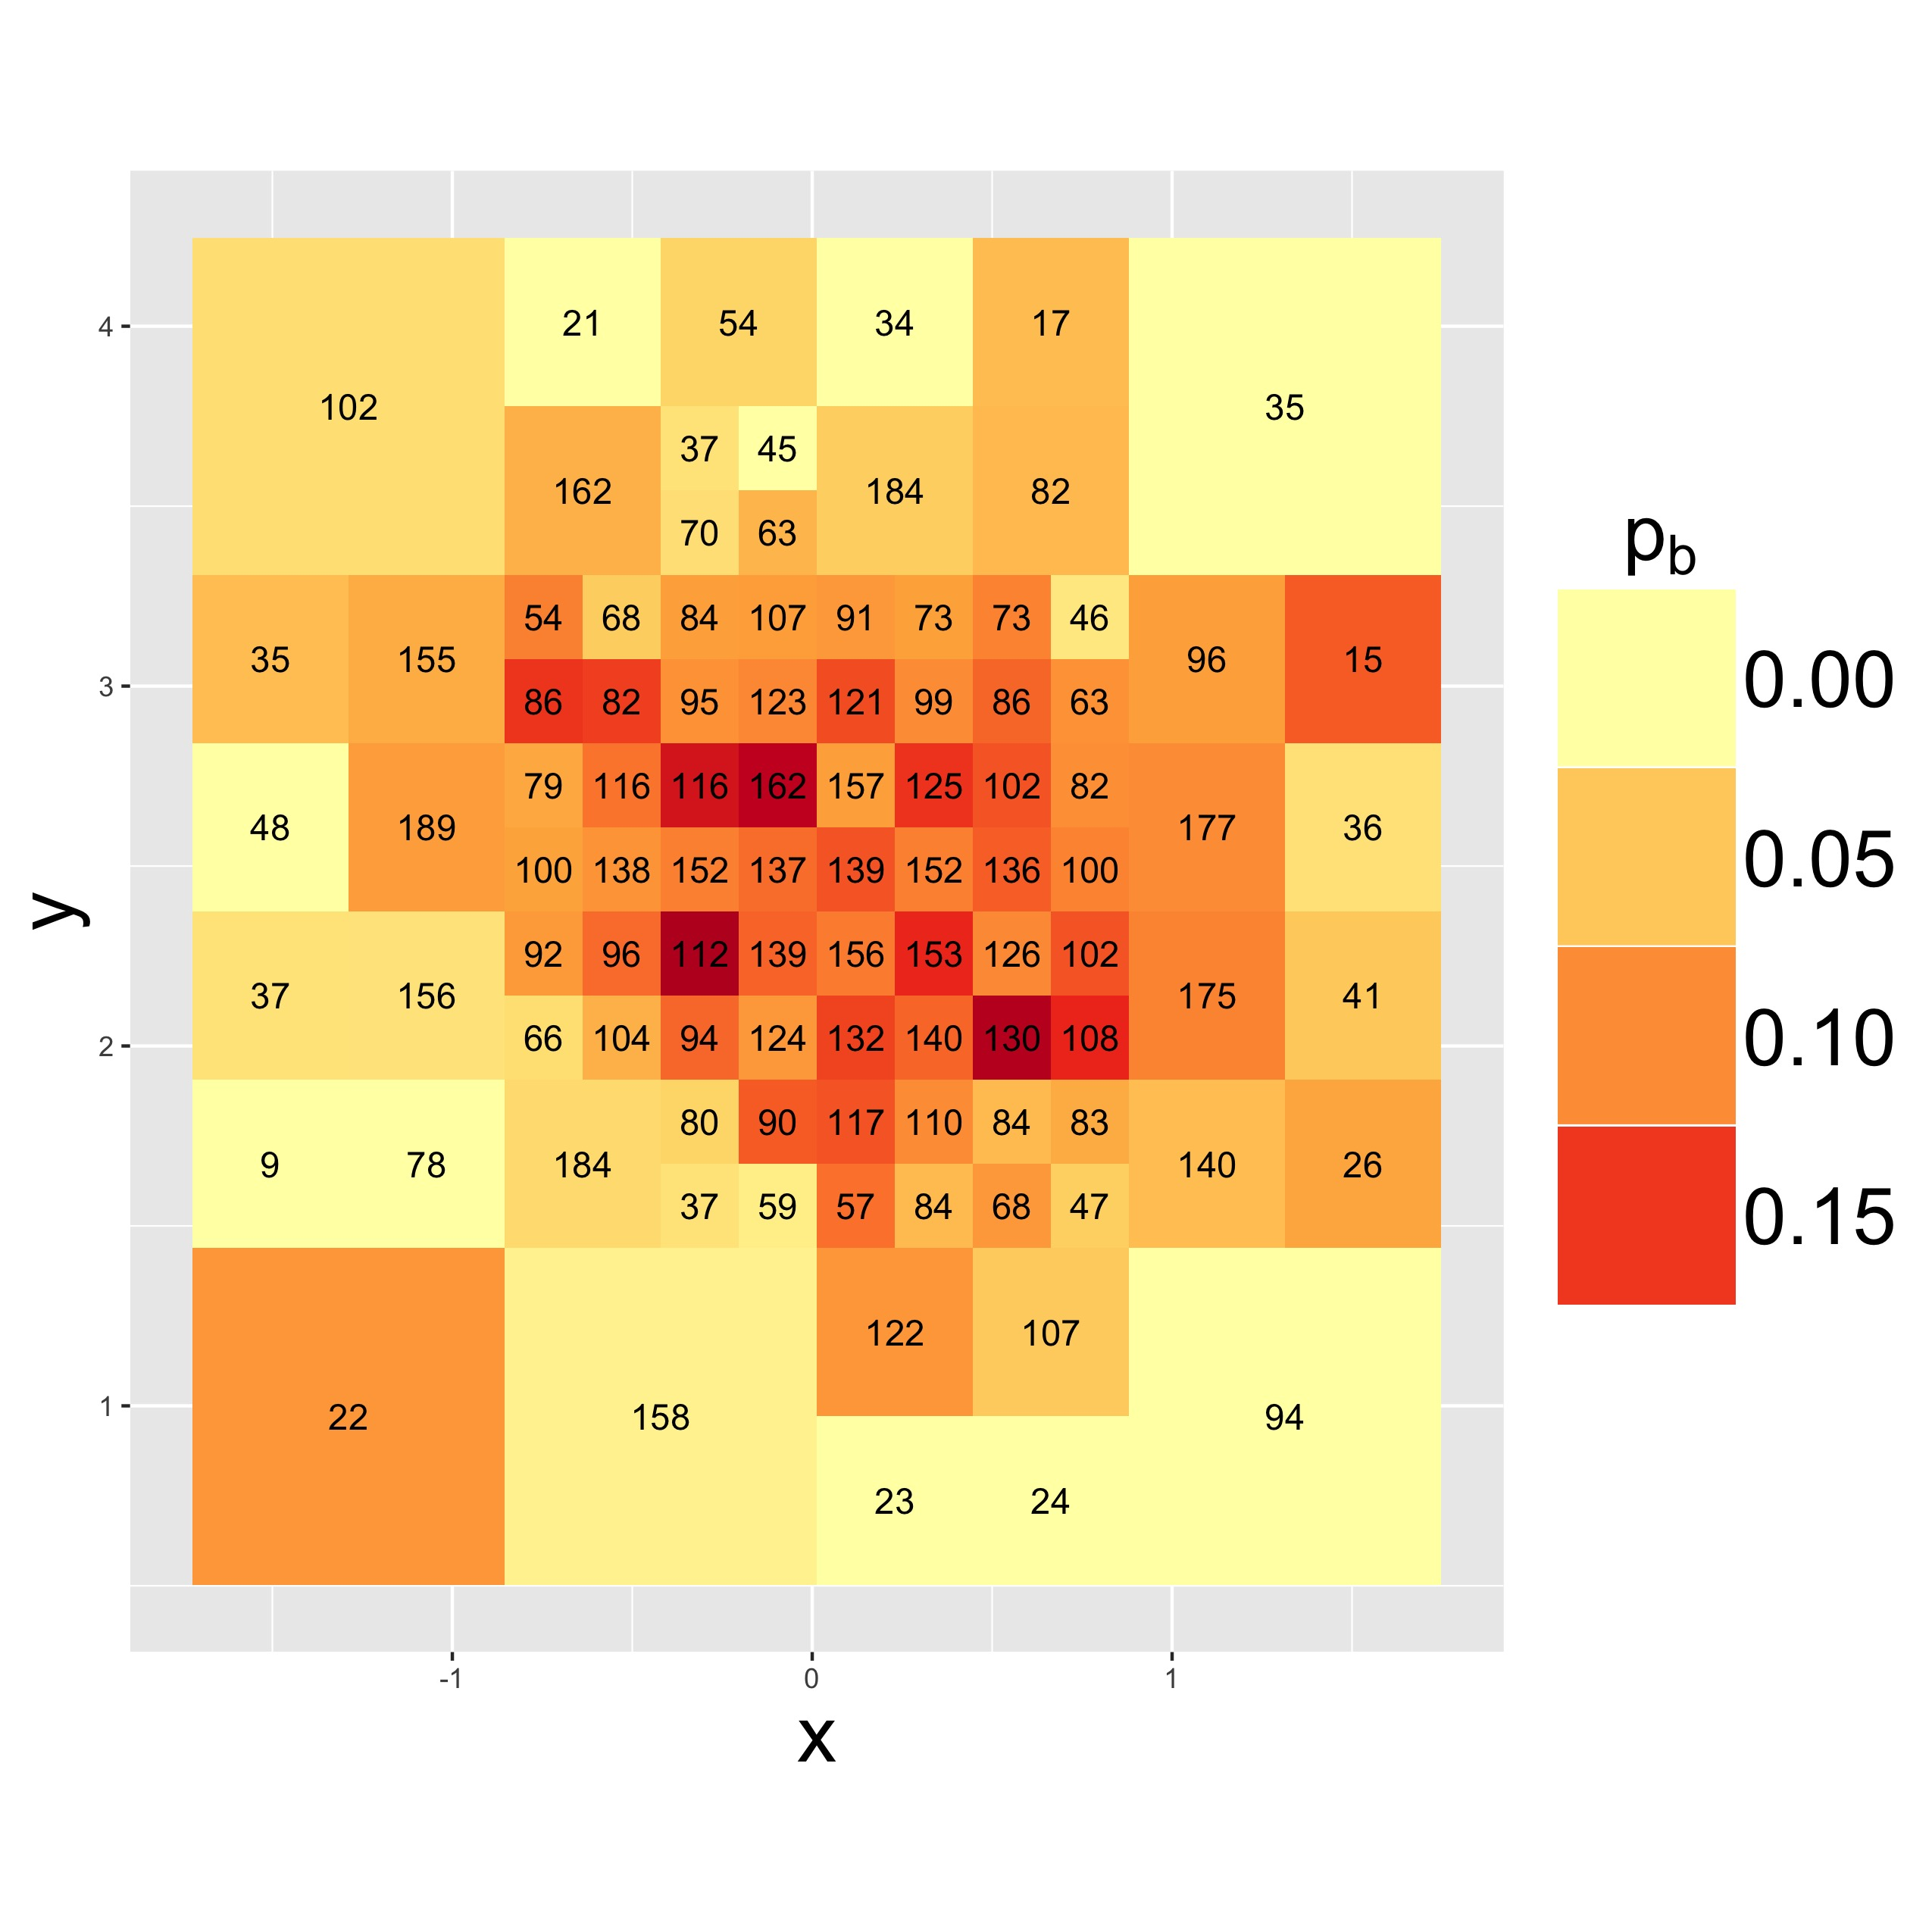
\includegraphics[scale=.05]{Images/Chapter16x16_200.jpg}
      	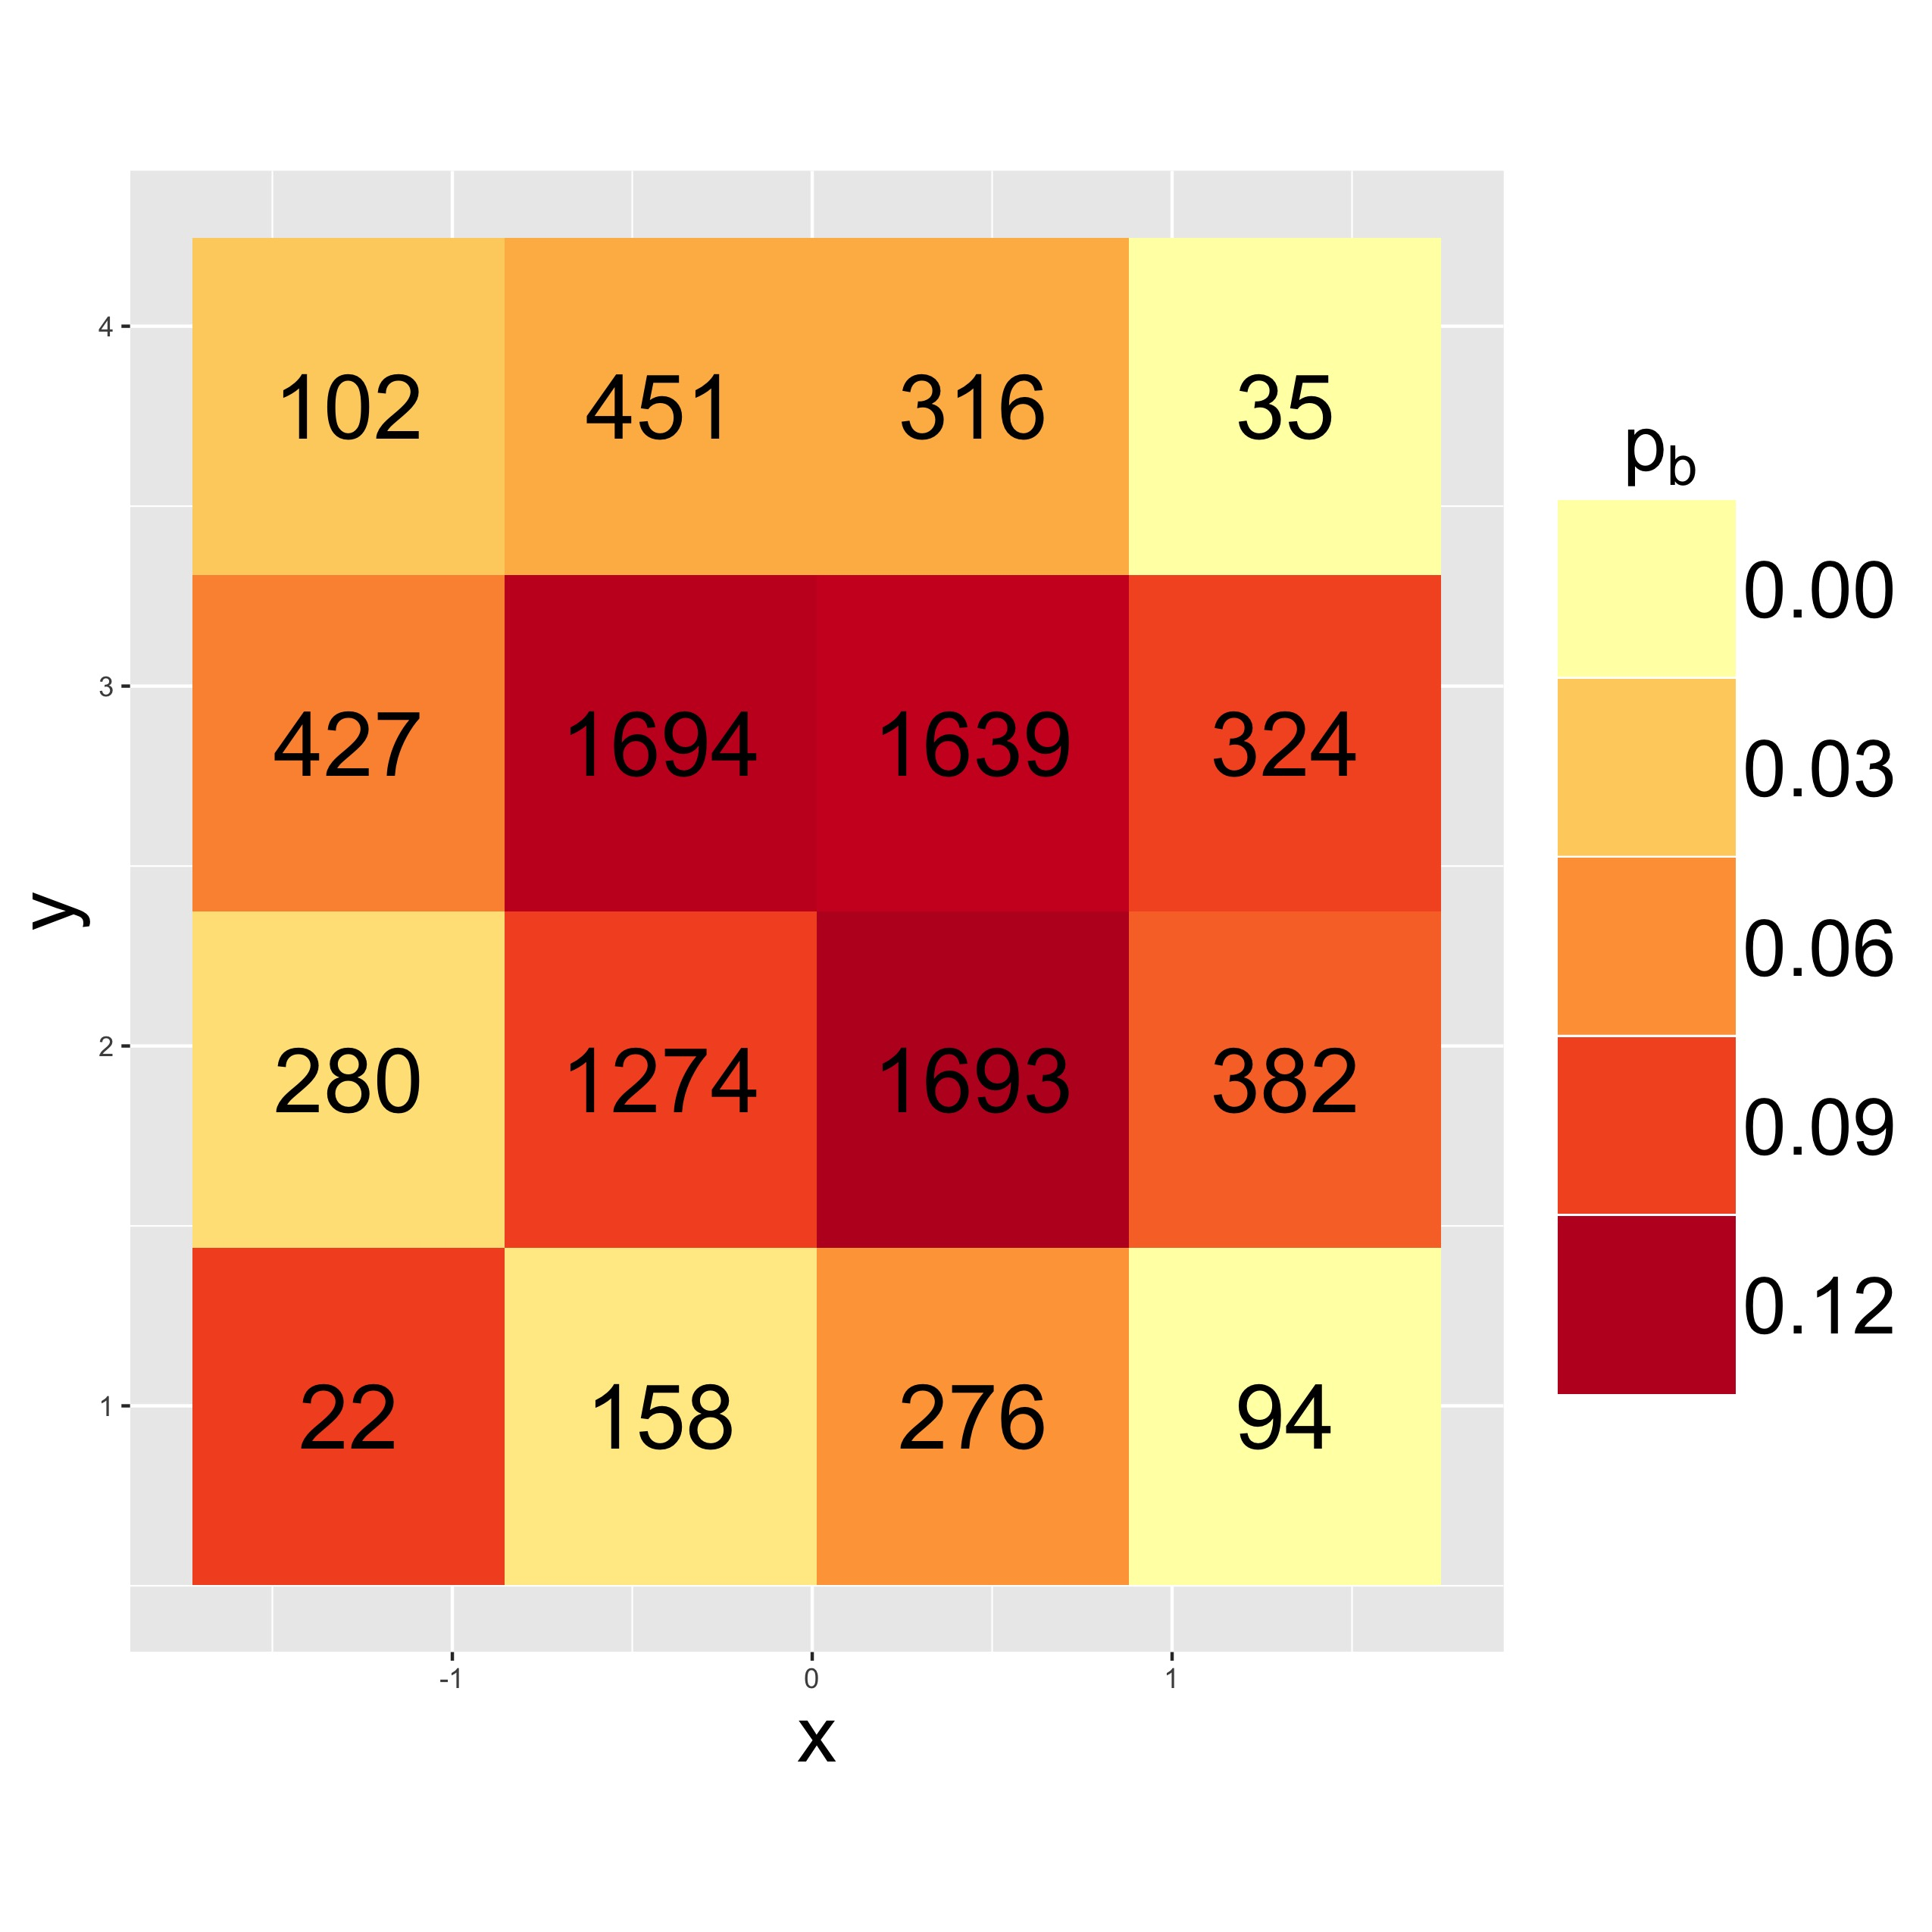
\includegraphics[scale=.05]{Images/Chapter4x4.jpg}
      	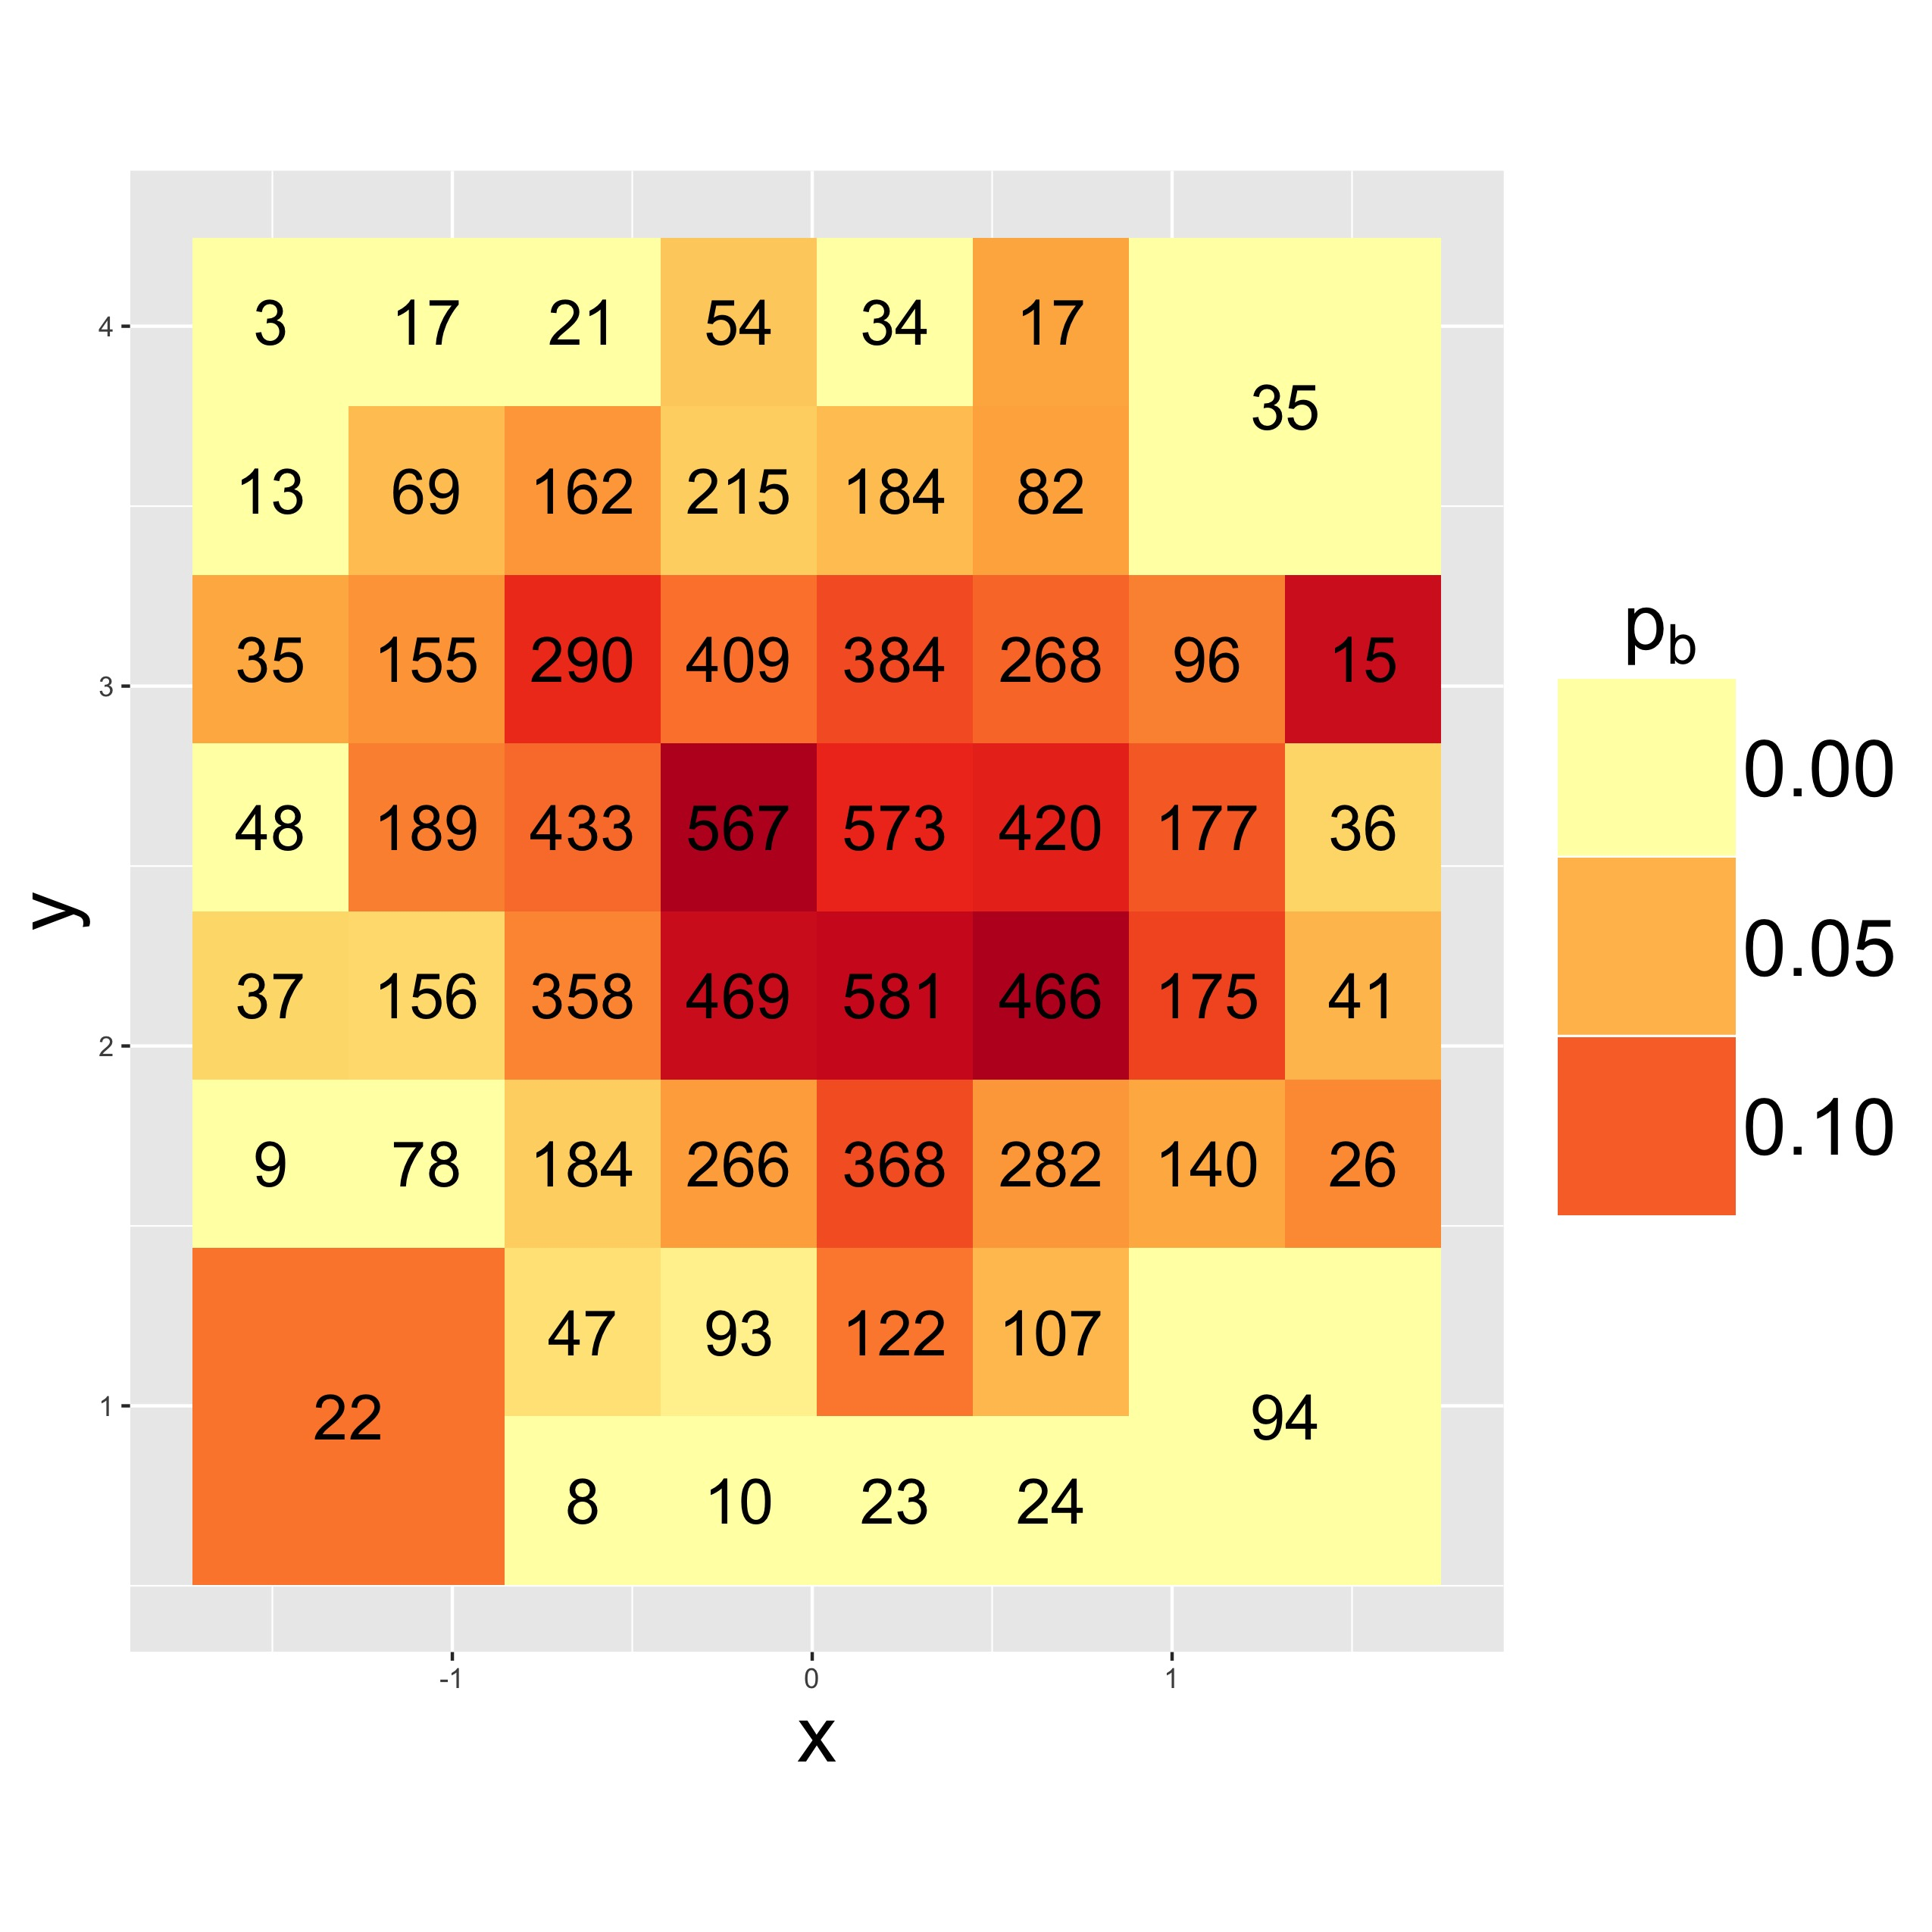
\includegraphics[scale=.05]{Images/Chapter8x8_100.jpg}
      	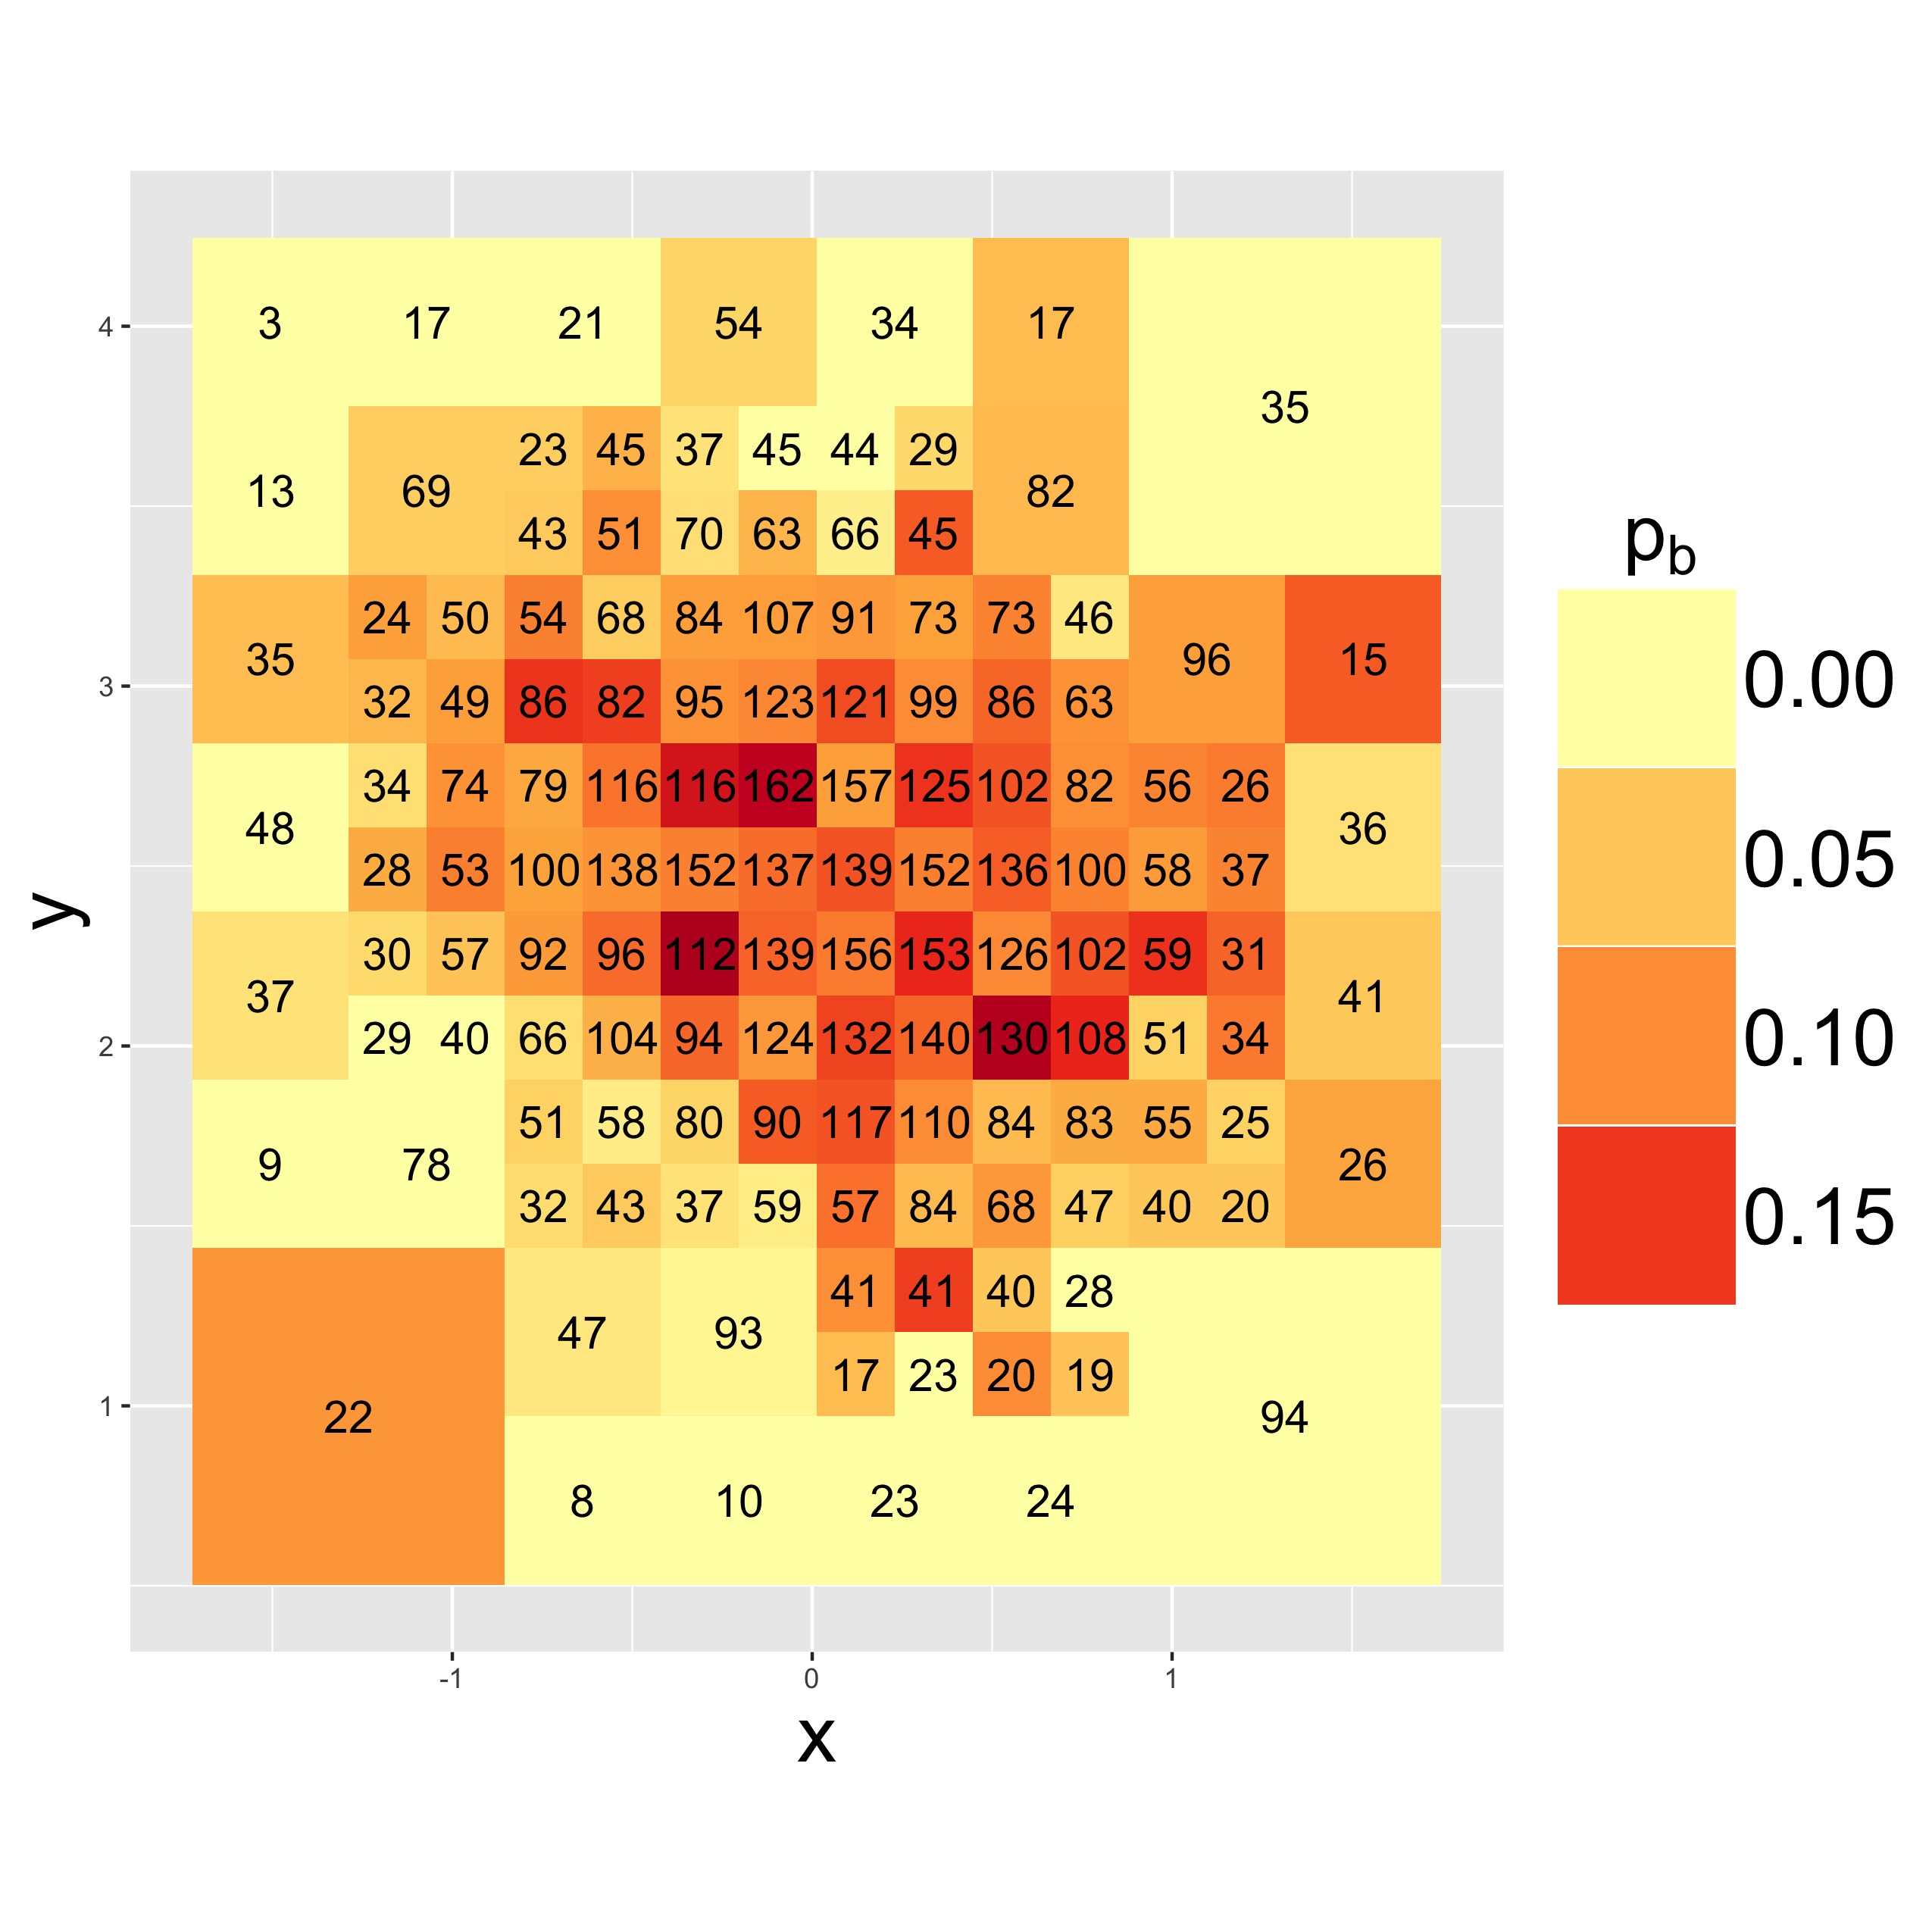
\includegraphics[scale=.05]{Images/Chapter16x16_100.jpg}
      	\caption{Variable-resolution heat maps diverge when box totals fall between sample size stopping rules. The top row of maps subdivides according to stopping rule $n_{b} < 200$; the bottom row further subdivides for stopping rule $n_{b} < 100$. The first three iterations produce identical maps, but then the sequences diverge as shown here.}
      	\label{fig:vrcomp2}
\end{figure}
For both stopping rules, notice how corner boxes tend to remain intact. This indicates Peralta swings less often at pitches in the strike zone corners, and/or less often sees such pitches. In the next section we delve into the possible reasons for this pattern, and others, in a baseball context.

\subsection{Interpretation: Hitter vs. Pitcher} % ==================

All-Star first basebman Keith Hernandez said the ``battle of wits... between the pitcher and hitter is baseball. Everything else is secondary.'' At the most basic level, the pitcher wants to get outs and avoid baserunners; and the hitter wants to avoid outs and get on base. There are two sides to every pitch's location: the pitcher's decision to throw there, and the hitter's decision to swing. In this section we look at two primary factors that influence these decisions in the battle of wits: game theoretic strategy, and pitch location execution error; and then use them to interpret a Peralta VR heat map.

\subsubsection*{Background}

Game theoretic strategy concerns the pitcher's knowledge of the hitter's strengths and weaknesses, and the hitter's reciprocal knowledge. For example, a pitcher prefers to avoid throwing pitches to the locations a hitter succeeds with the highest probability. In turn, the hitter would like to avoid swinging at pitches in locations he succeeds with relatively low probability.

Pitch location execution error refers to the fact that pitchers aim for the catcher's carefully positioned glove, but only rarely hit it exactly. More commonly the catcher moves his glove some distance to catch the pitch.  Analysis of this distance is impossible, because PITCHf/x\textsuperscript{\textregistered} data does not record the catcher's initial glove location. Therefore, without data to suggest otherwise, based on this author's own experience playing and watching baseball, for this discussion we pragmatically assume Normally distributed pitch location error, with $\mu = 0$ and $\sigma = 5$ inches, independently in the horizontal and vertical directions. 
\subsubsection*{Interpretation}

Now we use game theory and pitch location error to interpret aspects of a Peralta VR heat map. Figure \ref{fig:interp} shows Peralta's VR heat map for stopping rule $n_{b} < 200$.
        \begin{figure}[H]
      	\centering      
      	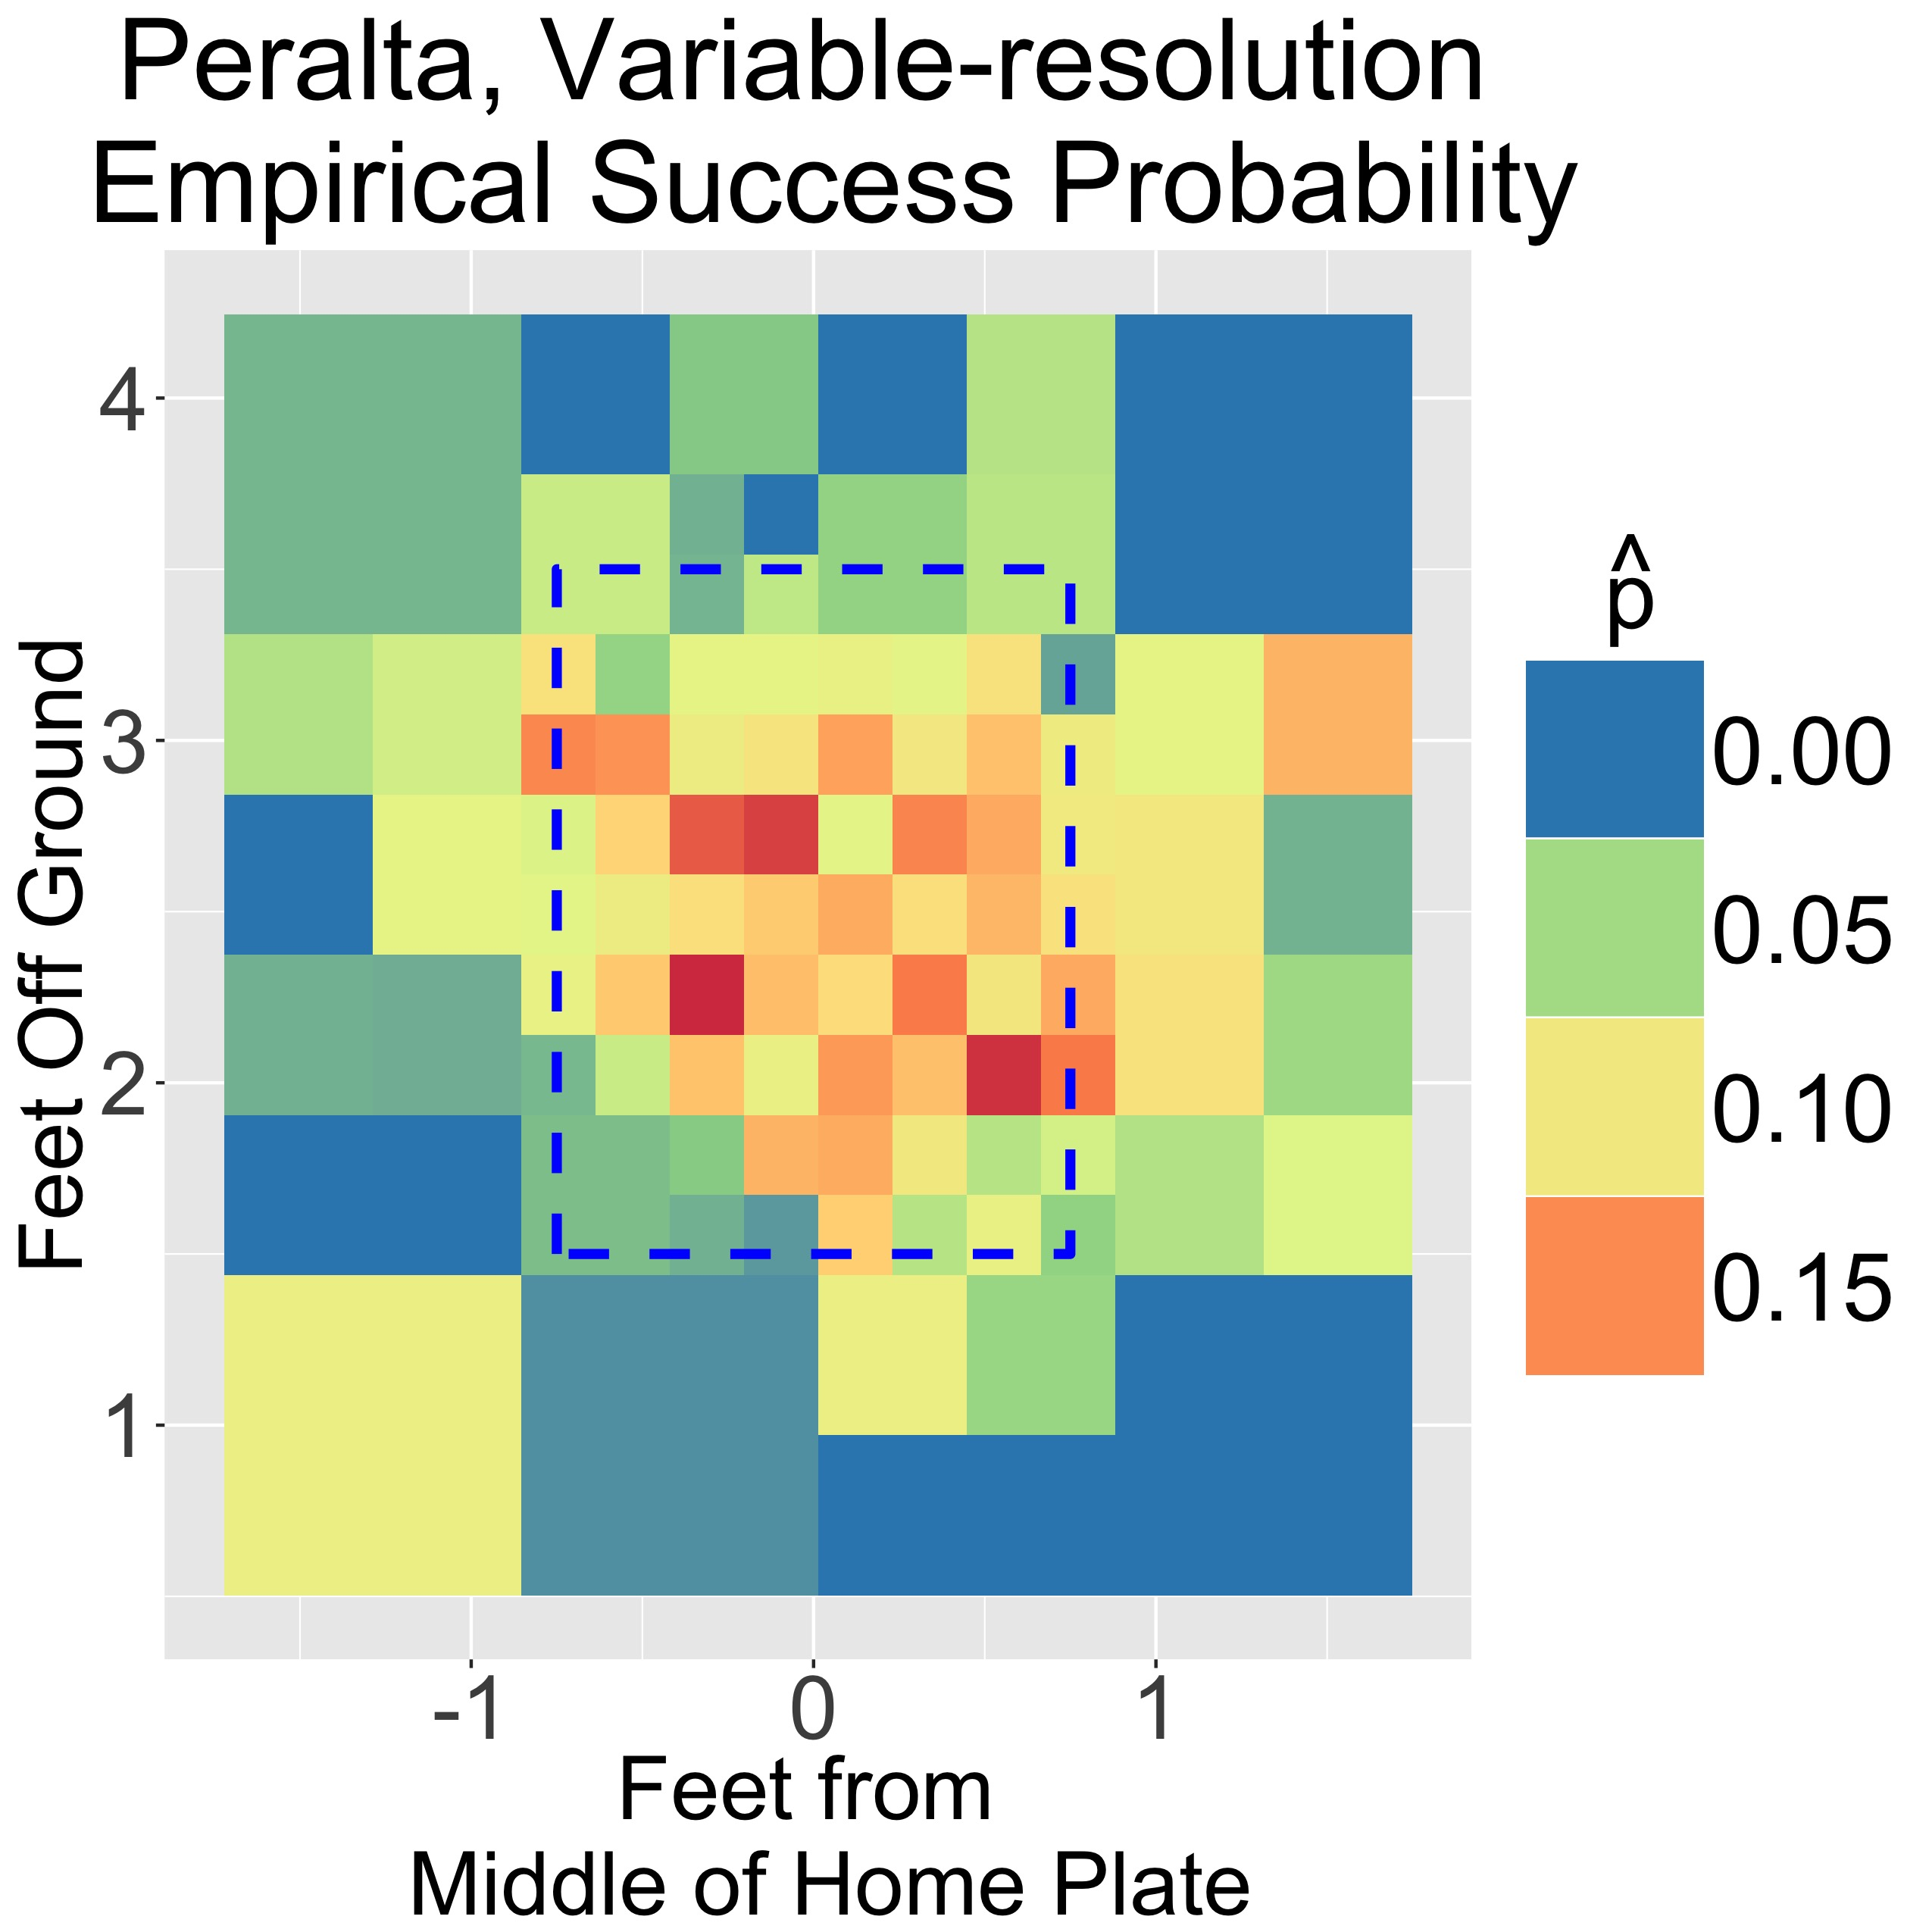
\includegraphics[scale=.1]{Images/Peralta_var-res.jpg}
      	\caption{This variable-resolution heat map for Jhonny Peralta gives spatial, empirical success probabilities; each box maps $\hat{b}_{b}$ to a color. In addition, the map conveys data density information; box size corresponds to the observation density, because subdivision persisted until box sample sizes dropped below 200.}
      	\label{fig:interp}
        \end{figure}
First, notice the grid boxes inside the dotted blue strike zone box tend to be smaller; this indicates Peralta generally saw and swung at far more pitches in the strike zone than out.\footnote{Please see the Appendix for the details and defintions of ball, strike, count, etc.} Pitchers throw pitches in the strike zone because each strike moves the at bat one step closer to an out; and each ball moves the at bat one step closer to a walk, where hitter proceeds to first base. The same logic, with reversed incentives, explains why Peralta swings at so many pitches in the strike zone. 

Second, notice the larger boxes in the lower left, upper left, and upper right of the strike zone. The larger boxes imply Peralta saw and/or swung at fewer pitches in these locations. To explain, consider a pitch aimed for the bottom left of the strike zone. Using the pitch location error distribution we assumed, aiming for this box yields a ball approximately 3/4 of the time, a result in the hitter's favor. From the hitter's perspective, these corner pitches are relatively difficult to hit, so Peralta presumably avoids swinging at them when possible. These two strategic considerations combined help explain low observation density in these locations.

Third, Peralta seems to have more success in the horizontal center of the strike zone, than at the top or bottom. This indicates Peralta deals with horizontal variation better than vertical variation---an actionable insight. Since Peralta swings at pitches in the middle of the strike zone almost every chance he gets, why do pitchers not avoid those locations? They probably tried. However, aiming for the middle of the strike offers the highest probability of a strike; missing the target by two standard deviations in any direction still yields a strike. In addition, some pitches aimed toward the margins of the strike miss their target and unintentionally pass through the middle of the strike zone. 

Finally, of the four corner locations just outside the strike zone, Peralta enjoyed the most success in the lower-left (yellow) box, with $\hat{p}_{b} = 0.10$. However, the size of this box indicates a relatively small sample size; either Peralta astutely swings at these challenging pitches infrequently, or pitchers may throw there infrequently because of the relatively greater risk: they less commonly induce swings, and non-swings move the at bat one step closer to a baserunner. 

VR heat maps also work well with other geostatistical data. In the next section we give an example of VR maps with marked point pattern data \citep{Schabenberger2004}.

\section{Example: Tornado Intensity}

\subsection{Background}

The National Weather Service, a division of the National Oceanic and Atmospheric Administration (NOAA), maintains seven National Centers for Environmental Protection. One of these, the Storm Prediction Center (SPC), collects tornado data, and provides it to the public at their website \citep{NOAA}. In this section we use SPC spatial tornado data, collected between 1950 and 2017, to show VR heat maps in another area of application. 

Meteorologists rate tornado intensity on the Fujita-scale (F-Scale), based primarily on tornado damage. The marked point pattern data set we use includes the longitude, latitude, and F-Scale rating for approximately 30,000 tornadoes in the last 67 years. Ordinarily this data would make resolution selection difficult, because tornado frequency varies greatly across the U.S. Low resolution appropriate for the Western U.S. would fail to convey available detail in the Midwest and West South Central division of the Southern U.S. \citep{regions}. High resolution appropriate for the latter regions would lead to sparsely populated grid boxes in the Western U.S. A VR heat map circumvents this challenge, and at the same time conveys the varying tornado frequency. 

\subsection{Variable-Resolution Map}

The VR heat map in Figure \ref{fig:tornado1}, created with stopping rule $n_{b} < 50$, shows the spatial average intensity, and relative frequency, of tornadoes.
        \begin{figure}[H]
      	\centering      
      	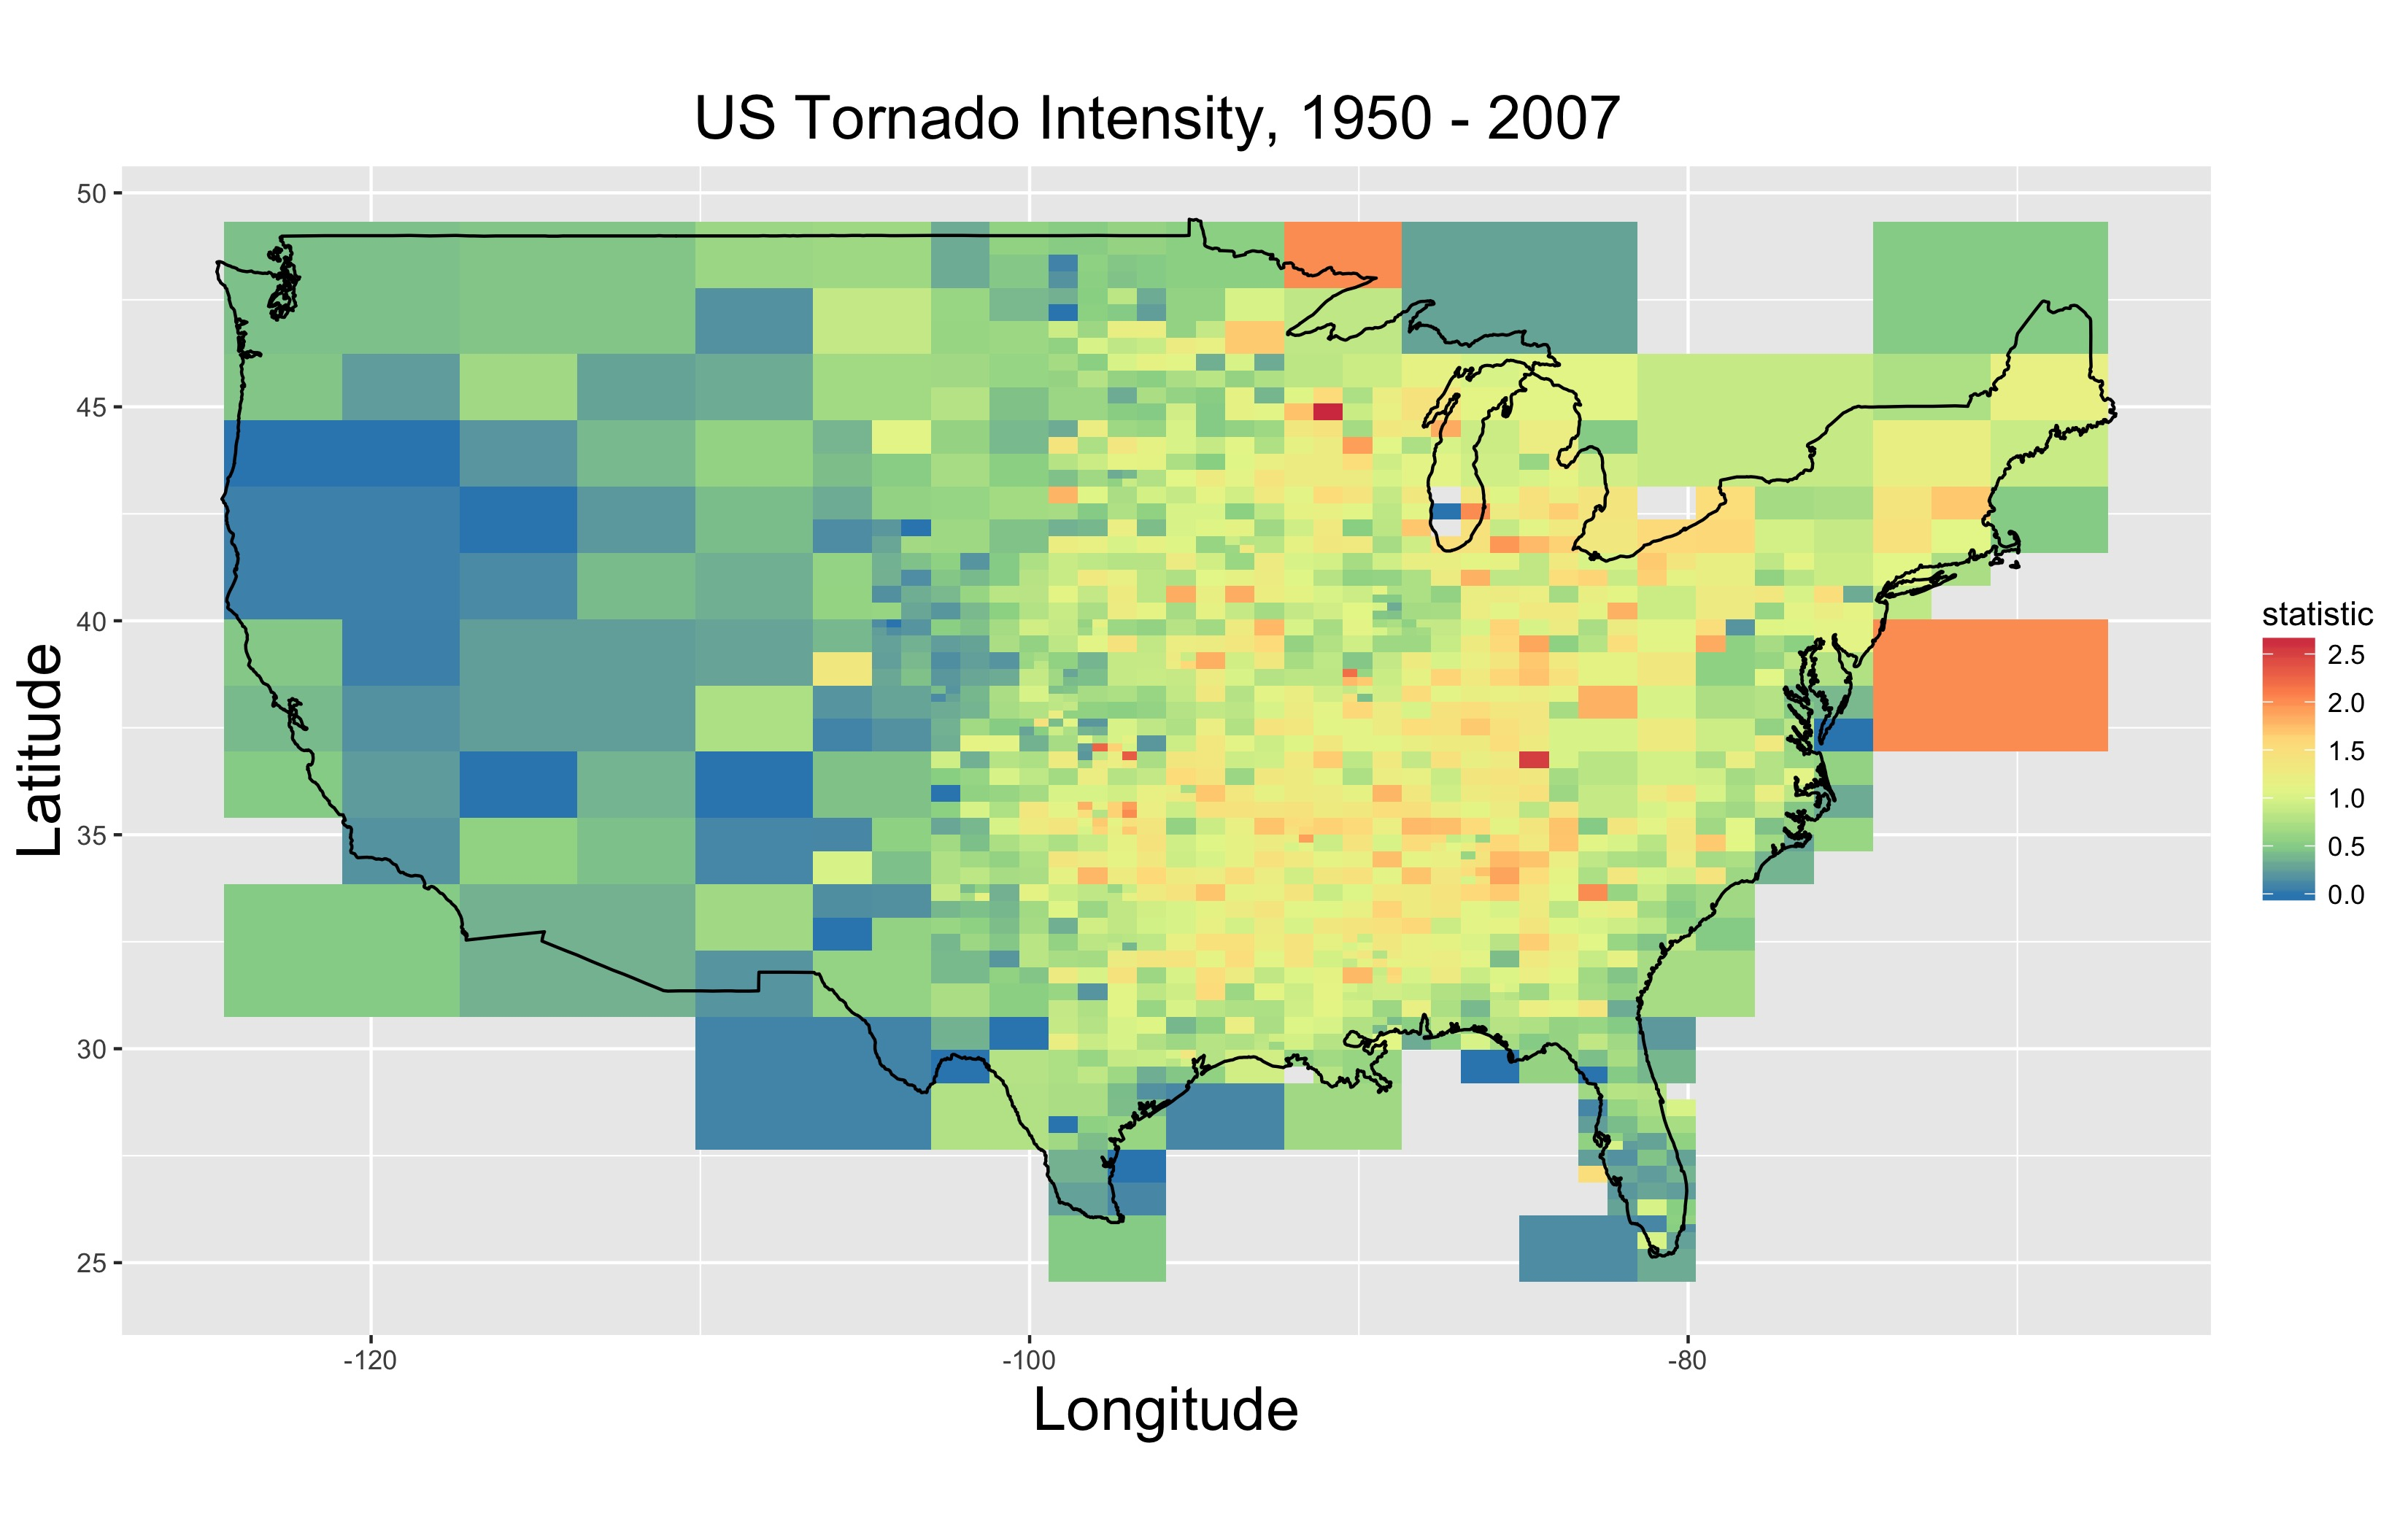
\includegraphics[scale=.14]{Images/vr_tornados.jpg}
      	\caption{This variable-resolution heat map shows tornado F-Scale intensity and frequency across the U.S. Each box maps average intensity to a color. Smaller (larger) boxes corresponds to higher (lower) observation density, because subdivision persisted until box sample sizes dropped below 50 tornadoes.}
      	\label{fig:tornado1}
        \end{figure}
Notice how the variable-resolution map conveys tornado frequency through grid box size, and seems to divide the country into three vertical regions. To the East of $-80^{\circ}$ West, medium-sized, largely green boxes indicate moderate tornado frequency and intensity. Between approximately $-80^{\circ}$ West and $-100^{\circ}$ West, tornado intensity and frequency increases, indicated by smaller, largely yellow boxes. Finally, moving further West, bigger, predominantly blue boxes indicate less frequent and less intense tornados than either of the previous two longitudinal ranges. The map performs well in these ways, but produces at least one peculiarity.

\subsection{Room for Improvement}

Notice how some grid boxes remain unnecessarily large, and awkwardly shaped relative to the U.S. borders. For example, a large horizontal rectangle overlaps Maine, in the North-eastern most corner of the U.S. This phenomenon occurs when an early iteration subdivision leaves a protruding quadrant with at least one observation, but fewer than the cutoff. The VR algorithm iterations in Figure \ref{fig:tornado2} show how the VR map evolves to its final form, but retains protruding boxes.
        \begin{figure}[H]
      	\centering      
      	\includegraphics[scale=.06]{Images/tornado_maps.jpg}
      	\caption{Variable-resolution (VR) algorithm iterations. The box colors represent average tornado F-Scale intensity, and the sequence shows the VR heat map evolution. Subdivision persists until box sample sizes drop below 50 (in this case) tornadoes in each box.}
      	\label{fig:tornado2}
        \end{figure}
The protruding box pattern occurred with boxes that protrude from, and partially overlap New Jersey, Southern Florida, Southern Texas, and Southern California. However, the size of these odd boxes does still indicate very low observation density, alerting the audience of the circumstance. Modifications to the algorithm---subdividing edge boxes with this quality---would eliminate this quirk.

\section{An R Package: {\it varyres}}